% vim:ts=4:sw=4
%
% Copyright (c) 2008-2009 solvethis
% Copyright (c) 2010-2015 Casper Ti. Vector
% Public domain.
%
% 使用前请先仔细阅读 pkuthss 和 biblatex-caspervector 的文档,
% 特别是其中的 FAQ 部分和用红色强调的部分。
% 两者可在终端/命令提示符中用
%   texdoc pkuthss
%   texdoc biblatex-caspervector
% 调出。

% 采用了自定义的(包括大小写不同于原文件的)字体文件名,
% 并改动 ctex.cfg 等配置文件的用户请自行加入 nofonts 选项;
% 其它用户不用加入 nofonts 选项,加入之后反而会产生错误。
%
% 图书馆要求电子版论文的目录必须为黑色,
% 且某些教务要求打印版论文的文字部分为纯黑色而非灰度打印,
% 【因此最终打印和提交论文前,请将“colorlinks”改为“nocolorlinks”。】
\documentclass[UTF8, colorlinks]{pkuthss}

% 使用 biblatex 排版参考文献,并规定其格式(详见 biblatex-caspervector 的文档)。
% 这里按照英文文献在前,中文文献在后排序(“sorting = ecnty”);
% 若需按照中文文献在前,英文文献在后排序,请设置“sorting = centy”;
% 若需按照引用顺序排序,请设置“sorting = none”。
\usepackage[backend = biber, style = caspervector, utf8, sorting = none]{biblatex}
% 提供近似于学校所要求的 Times New Roman / Arial 的字体。
\usepackage[defaultsups]{newtxtext}
\usepackage{newtxmath}
% 产生 originauth.tex 里的 \square。
\usepackage{latexsym}

% 按学校要求设定参考文献列表中的条目之内及之间的距离。
\setlength{\bibitemsep}{3bp}
% 对于 linespread 值的计算过程有兴趣的同学可以参考 pkuthss-extra.sty。
\renewcommand*{\bibfont}{\zihao{5}\linespread{1.27}\selectfont}

% 设定文档的基本信息。
\pkuthssinfo{
    cthesisname = {硕士研究生学位论文}, ethesisname = {Doctor Thesis},
    ctitle = {面向高速路网的关键路段识别研究}, etitle = {Test Document},
    cauthor = {刘丹萌},
    eauthor = {Test},
    studentid = {1401214385},
    date = {2017年5月10日},
    school = {北京大学},
    cmajor = {计算机科学与技术(智能科学与技术)}, emajor = {Some Major},
    direction = {数据仓库与数据挖掘},
    cmentor = {宋国杰}, ementor = {Prof.\ Somebody},
    ckeywords = {复杂网络,高速公路,关键节点,社群划分}, ekeywords = {Complex network, Highway,Key node,Community}
}
% 载入参考文献数据库(注意不要省略“.bib”)。
\addbibresource{thesis.bib}

% 普通用户可删除此段。
\usepackage{algorithm}  
\usepackage{algorithmicx} 
\usepackage{algpseudocode}
\usepackage{bm}
\usepackage{color}
\def\pkuthssffaq{%
	\emph{\textcolor{red}{pkuthss 文档模版最常见问题:}}

	在最终打印和提交论文之前,
	请将 pkuthss 文档类选项中的 %
	\texttt{colorlinks} 替换为 \texttt{nocolorlinks},
	因为图书馆要求电子版论文的目录必须为黑色,
	且某些教务要求打印版论文的文字部分为纯黑色而非灰度打印。

	\texttt{\string\cite}、\texttt{\string\parencite} %
	和 \texttt{\string\supercite} 三个命令分别产生%
	未格式化的、带方括号的和上标且带方括号的引用标记:%
	\cite{test-en},\parencite{test-zh}、\supercite{test-en, test-zh}。

	若要避免章末空白页,请在调用 pkuthss 文档类时加入 \texttt{openany} 选项。

	如果编译时不出参考文献,
	请参考 \texttt{texdoc pkuthss}“问题及其解决”一章
	“其它可能存在的问题”一节中关于 biber 的说明。
}

\begin{document} \large
	% 以下为正文之前的部分,默认不进行章节编号。
	\frontmatter
	% 此后到下一 \pagestyle 命令之前不排版页眉或页脚。
	\pagestyle{empty}
	% 自动生成封面。
	\maketitle

	% 此后到下一 \pagestyle 命令之前正常排版页眉和页脚。
	% 封面要求单面打印,故需新开右页,此处已一并实现。
	\cleardoublepage
	\pagestyle{plain}
	% 重置页码计数器,用大写罗马数字排版此部分页码。
	\setcounter{page}{0}
	\pagenumbering{Roman}

	% 版权声明。
	% vim:ts=4:sw=4
%
% Copyright (c) 2008-2009 solvethis
% Copyright (c) 2010-2014 Casper Ti. Vector
% All rights reserved.
%
% Redistribution and use in source and binary forms, with or without
% modification, are permitted provided that the following conditions are
% met:
%
% * Redistributions of source code must retain the above copyright notice,
%   this list of conditions and the following disclaimer.
% * Redistributions in binary form must reproduce the above copyright
%   notice, this list of conditions and the following disclaimer in the
%   documentation and/or other materials provided with the distribution.
% * Neither the name of Peking University nor the names of its contributors
%   may be used to endorse or promote products derived from this software
%   without specific prior written permission.
%
% THIS SOFTWARE IS PROVIDED BY THE COPYRIGHT HOLDERS AND CONTRIBUTORS "AS
% IS" AND ANY EXPRESS OR IMPLIED WARRANTIES, INCLUDING, BUT NOT LIMITED TO,
% THE IMPLIED WARRANTIES OF MERCHANTABILITY AND FITNESS FOR A PARTICULAR
% PURPOSE ARE DISCLAIMED. IN NO EVENT SHALL THE COPYRIGHT HOLDER OR
% CONTRIBUTORS BE LIABLE FOR ANY DIRECT, INDIRECT, INCIDENTAL, SPECIAL,
% EXEMPLARY, OR CONSEQUENTIAL DAMAGES (INCLUDING, BUT NOT LIMITED TO,
% PROCUREMENT OF SUBSTITUTE GOODS OR SERVICES; LOSS OF USE, DATA, OR
% PROFITS; OR BUSINESS INTERRUPTION) HOWEVER CAUSED AND ON ANY THEORY OF
% LIABILITY, WHETHER IN CONTRACT, STRICT LIABILITY, OR TORT (INCLUDING
% NEGLIGENCE OR OTHERWISE) ARISING IN ANY WAY OUT OF THE USE OF THIS
% SOFTWARE, EVEN IF ADVISED OF THE POSSIBILITY OF SUCH DAMAGE.

\chapter*{版权声明}
{
	\zihao{3}\linespread{1.5}\selectfont

	任何收存和保管本论文各种版本的单位和个人,
	未经本论文作者同意,不得将本论文转借他人,
	亦不得随意复制、抄录、拍照或以任何方式传播。
	否则一旦引起有碍作者著作权之问题,将可能承担法律责任。
	\par
	% 若需排版二维码,请将二维码图片重命名为“barcode”,
	% 转为合适的图片格式,并放在当前目录下,然后去掉下面 3 行的注释。
	%\vfill\noindent
	%\includegraphics[height = 5em]{barcode}
	%\par
}


	% 中英文摘要。
	% vim:ts=4:sw=4
% Copyright (c) 2014 Casper Ti. Vector
% Public domain.

\begin{cabstract}
	% 中文测试文字。

		交通问题是当今世界关注的热点问题。随着人们生活水平的提高、交通系统的发展,社会交通需求也日益增大。交通与环境、交通与能源、交通与需求之间的矛盾日益加剧,交通事故和堵塞给人们带来了巨大的效率、能源和生命上的损失,简单的交通控制技术已经不能满足需求。传统智能交通研究以路网中的单个空间位置点为研究对象,运用动力学,统计学,仿真学与机器学习相关理论对其交通流行为进行分析。随着交通系统的不断发展,交通系统逐渐呈现网络化态势,路网中各个节点之间紧密联系,单个空间位置点的研究已经不足以描述整个高速公路路网的宏观特性。随着交通事故逐渐成为交通系统的瓶颈所在,智能交通系统的研究出现了新的需求:如何找到交通系统中的关键节点,通过对这些关键节点进行处理,以达到减少交通路网瘫痪率、增加路网运行稳定性的目的。

		在网络化的智能高速公路系统中,关键节点的研究集中在1)对交通网络拓扑结构的研究;2)对交通网络信息进行统计研究;3)利用传播动力学,对微观站点进行相关研究。我们的目的是找到关键节点,在整体网络中提升运行效率,方法1)只针对了路网的拓扑结构,没有考虑节点之间的信息交流;方法2)基于传统统计学,并在统计学的基础上,利用数据挖掘方法研究关键节点,路网中的车流流量随时间变化而变化,该方法只能静态分析路网关键节点,无法分析关键节点随着时间/路网流量的变化规律;方法3)集中研究微观领域的交通特性,对整体路网的研究意义不大。在此我们提出一种基于宏观高速公路网络的目标模型,根据选取节点对模型的影响,选取关键节点。为了深入挖掘高速公路关键节点特性,我们提出了一个较复杂的概率求解模型。这个模型直接求解时间复杂度高,不符合智能交通系统的实时应用需求。基于复杂网络的小世界特性,在此引入高速公路网络的分群算法,进行分治处理

		因此,本文从智能交通的实际应用需求出发,针对现有关键节点挖掘研究方法的不足,深入进行两个方面的研究:提出一种描述语高速公路的关键节点与高速公路的通行状况之间联系的函数模型,针对现有复杂网络关键节点研究的局限性,从宏观层面提出目标函数,结合高速公路的实时路况,研究实时高速公路中关键节点的位置;提出一种基于高速公路路网的社群划分方法。针对现有社群划分方法中的分辨率限制与极端退化特性,结合高速公路路网的特点,建立适用于高速公路的社群划分模型,在一定程度上解决传统方法中的分辨率限制与极端退化特性。

        本文的贡献主要有以下几点:
        
		(1)提出一种高速公路路网关键节点挖掘模型,突破现有复杂网络的局限性
		
		(2)提出一种基于高速公路路网的社群划分模型,降低高速公路关键节点挖掘复杂度,使得方法可以实际应用。
\end{cabstract}

\begin{eabstract}
	Traffic problem is a hot issue in the world today. With the improvement of people's living standard and the development of the traffic system, the demand of social traffic is increasing day by day. The contradiction between traffic and environment, transportation and energy, traffic and demand increasing, traffic accidents and congestion brings efficiency, energy and life in the great loss, simple traffic control technology has been unable to meet the demand. The study of the traditional intelligent transportation is based on the research of the single spatial location in the road network, which is based on the theory of dynamics, statistics, simulation and machine learning. With the continuous development of the traffic system, traffic system gradually presents the network situation, the close connection between each node in the network, the macro characteristics of single point position is not enough to describe the whole Expressway network. With the traffic accident has become the bottleneck of the traffic system, the research of intelligent transportation system has new demand: how to find the key nodes in the traffic system, by processing the key nodes, in order to reduce the traffic paralysis rate, increase the operation stability of road network to.
	
	In the intelligent highway system network, the research focused on 1 key nodes) study on traffic network topology; 2) for statistical research on traffic network information; 3) using the propagation dynamics, the research of micro site. Our purpose is to find the key nodes in the network, improve the efficiency in the whole network, method 1) only for the topology of the network, do not consider the exchange of information between nodes; 2) based on the traditional statistical methods, and on the basis of statistics, using data mining method of key nodes, and the change in the flow of network traffic change over time, this method can only static analysis of network key nodes, to analysis of key nodes changes with time and network flow method; 3) focus on the traffic characteristics of the micro field, the whole road network is of little significance. In this paper, we propose a target model based on macroscopic Expressway network. In order to deeply explore the key nodes of freeway, we propose a more complex probabilistic model. This model has high time complexity and can not meet the requirement of real-time application of intelligent transportation system. Based on the small world characteristics of complex networks, this paper introduces the clustering algorithm of expressway network, which is divided into four parts
	
	Therefore, this article from the intelligent transportation according to the practical requirement, aiming at the key nodes of mining lack of research methods, in-depth study of two aspects: the function model between the key nodes and highway traffic conditions put forward a description of expressway, aiming at the limitations of existing key nodes of the complex network, put forward the objective function from the macro level, combined with real-time traffic highway, on key nodes in the expressway real-time position; proposes a classification method of highway network based on community. The resolution limit and extreme for the existing community division method in the degradation characteristics, combined with the characteristics of the highway network, community partition model is established by the highway, to a certain extent to solve the resolution limitation of the traditional method and extreme degradation characteristics.
	
	The main contributions of this paper are as follows:
	
	(1)In this paper, a new model of key nodes in highway network is proposed, which breaks through the limitations of existing complex networks
	
% 	(2)In this paper, a new model of community partition based on expressway network is proposed, which can reduce the complexity of the key nodes and make the method practical.
\end{eabstract}


	% 自动生成目录。
	\tableofcontents
	\listoffigures

	% 以下为正文部分,默认要进行章节编号。
	\mainmatter
	% 序言。
	% vim:ts=4:sw=4
% Copyright (c) 2014 Casper Ti. Vector
% Public domain.

\chapter{引言}
% 中文测试文字。
\section{研究背景}
\subsection{高速公路交通研究背景}

高速公路网络已经成为支撑国家经济发展、服务群众生活、保障国家安全的战略资源和设施。截止2016年底,我国公路通车总里程达到457万公里,其中高速公路12万公里,2017年将新增4500公里,是世界上规模最大的高速公路网络(如图\ref{gaosugonglu}所示)。 

				\begin{figure}[h]
				\centering
						\begin{minipage}{0.8\linewidth}
							\centering
							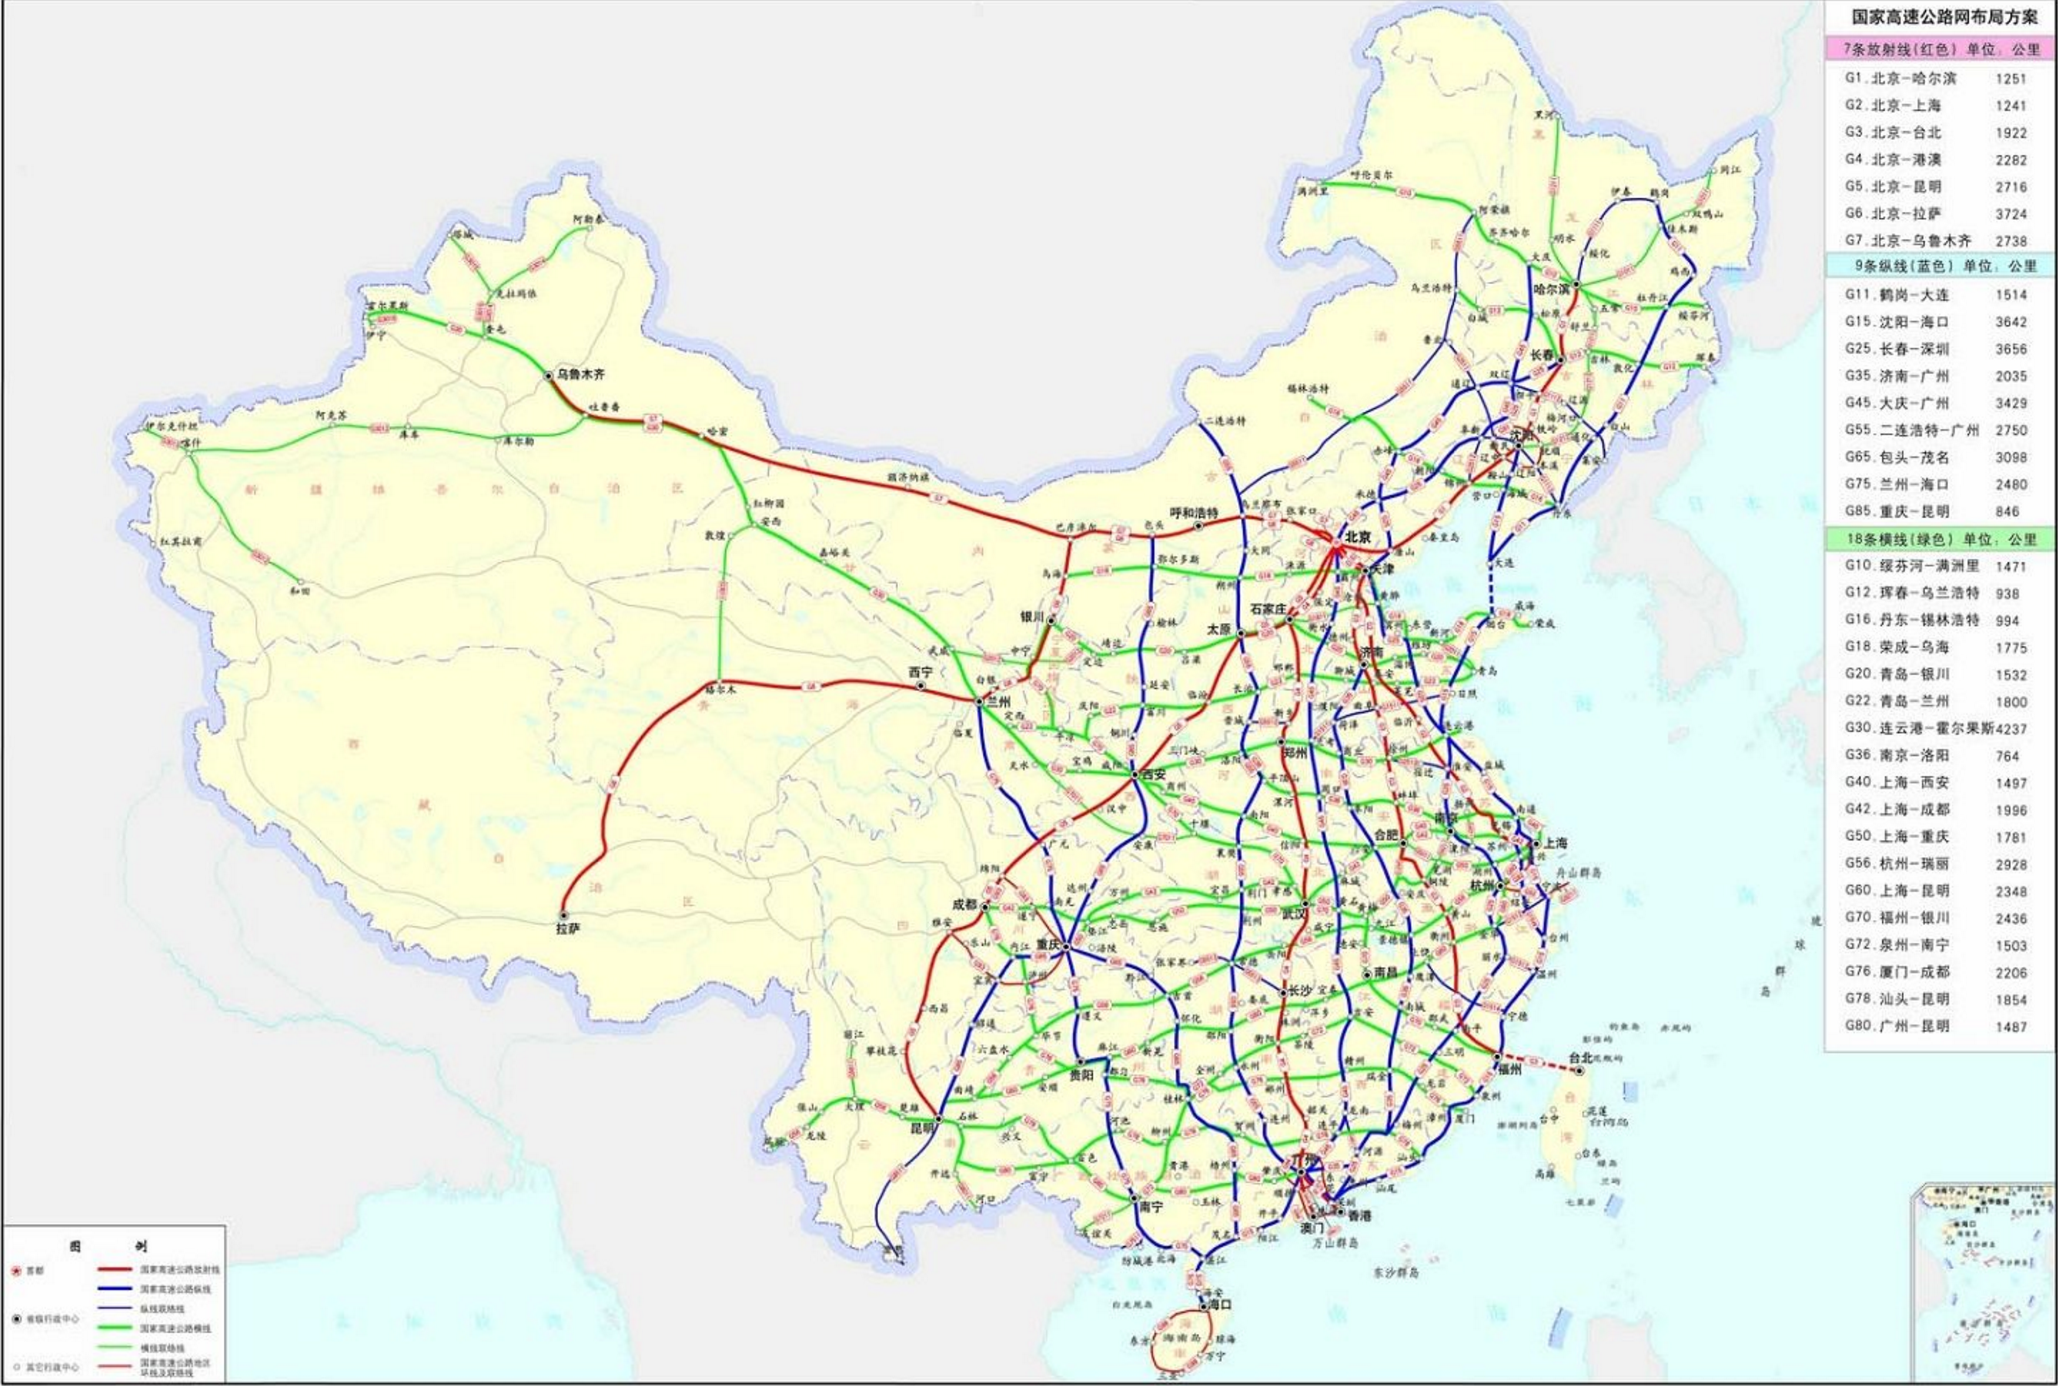
\includegraphics[width=4.4in]{picture/gaosugonglu}
							\caption{fig1}
							\label{gaosugonglu}
						\end{minipage}%\
				\end{figure}

随着中国经济的快速发展,人们生活水平的不断提高,居民的出行和货物运输的数量也在逐渐增加。交通系统是人类活动不可缺少的一部分。据估计,每天平均有40\%的人口在路上花费至少1小时。近几年来,人们变得越来越依赖于交通系统,对于交通系统管理人员来说,机遇和挑战共存。首先,交通拥堵已成为一个日益严重的问题。全球范围内的道路上的车辆增加,根据调查,截止至2016年初,北京共有544万辆车,比2014年初增加了50万辆。这些激增的车辆会对道路系统产生严重的压力,极大的增加拥堵以及拥堵后的损耗。拥堵会导致燃油消耗增加,空气污染,以及实施公共交通计划的困难。车流流量过多时,交通事故风险与交通运输系统中的膨胀增加,交通事故之后的恢复时间与恢复代价也会急剧增加。在中国,2009年的交通事故死亡人数约有7万人,在2015年达到9万人。美国联邦公路管理局公布的报告显示,发生在城市的交通事故约占所有拥堵延误的50\% - 60\%。毫无疑问,如何高效处理交通事故和预测事故发生点,一旦世故发生,最大限度地减少其影响是一个核心问题。由于资源相对有限,尤其是中国高速公路正在逐渐走向免费,因此很难有预算全面建立新的基础设施。同时,运输系统的有效性也越来越依赖于一个国家的处理紧急情况的能力(例如,大规模疏散和安全增强)。一个国家的技术竞争力,其经济实力和生产能力,在很大程度上取决于其交通系统性能。随着高速公路的不断发展,各类维护高速公路的需求也都被一一提出,示例如下:

1)人员分配。最典型的是今年五一,山东高速管理人员联合曲阜路政大队、济宁京台高速交警大队、项目部制定有针对性的应急预案,根据历史的交通信息,负责做好恶劣天气、旅游高峰车流量饱和、突发事件引起交通阻塞的应急处理。安排值班人员,落实机械设备和应急物资准备,一旦发生突发事件,迅速启动,切实做好节日期的保畅工作。

2)安全管理。面对节日期间可能出现的状况,高速公路养护所需要在节日前期组织开展道路安全隐患检查活动:一是对管段路段进行安全隐患排查,发现问题立即落实整改;二是加强春季防火工作的管理,及时清理桥涵构造物下的易燃物品,对边坡、中央分隔带进行打草、苗木修剪,对匝道圈进行专人看护,安排养护员负责所辖路段的防火报警工作。

3)基础设施建设。交通的基础设施建设主要包括交通轨道交通设施建设、停车场设施建设等。交通基础设施包括为交通系统保障安全正常运营而建设的公路、轨道、隧道、高架道路、车站、通风亭、机电设备、供电系统、通信信号、道路标线等设施。

4)高新设施建设。目前越来越多的新技术涌现,比如说最近成都绕城高速公路的部分路段的养护施工采用了新技术——“就地热再生”。这是目前国际上先进的沥青路面施工技术,具有高效、优质、环保、节约的特点,施工过程中采用的是单车道施工方式,施工时占用的工作面小,不中断交通,施工完半小时路面温度降至50摄氏度即快速开放交通。同时就地热再生施工相比传统工艺,在温室气体排放量方面,每施工1万平方米可减少二氧化碳排放26吨,在资源的利用率方面,每施工1万平方米利用废旧沥青混合料960吨,节约新沥青料600吨。就地热再生方法在节能环保、废旧沥青再利用方面的优势在本次绕城高速施工中显现。

上述需求中有一个共性的问题,那就是如何找出高速公路网络中最重要的路段,然后针对这些重要路段,进行针对性管理。高速公路的变化日新月异,根据经验很难非常准确的预估出所有关键路段。亟需提出一套适用于大规模路网的高速公路的关键路段挖掘识别系统。在识别高速公路网络中关键路段的前提下,我们可以进行有效的人员分配,避免人员浪费;可以针对高危路段进行安全管理,减少事故风险;可以针对具有强烈需求的路段进行基础设施建设,避免资源浪费,也可以研究当关键路段因为施工等原因停滞时,如何将影响减少到最小。

本文提出的面向高速公路的关键路段挖掘模型就是一种为了满足上述需求而提出的模型。本文将重点分析高速公路网络的网络特点,以路段/网络运行效率模型为评价标准,在宏观层面上提出一种高速公路重要节点的挖掘模型,同时分析其模型性质,提出一种优化策略。从整体路网的流量角度提出适用于中国高速公路的大规模高速公路网络的关键路段识别算法。

本文针对高速公路进行关键节点挖掘,主要基于高速公路收费数据,并得到如下项目的支持:

1)



\subsubsection{网络性}
    纵横交错的道路构成了复杂的交通路网,这使得交通系统具有了网络性质。网络中,不同的收费站构成了节点,相邻收费站之间的道路构成了网络中的边,节点之间通过车辆来交流。高速公路网络化,使得交通系统中的车流行为更加复杂,这对交通研究方法提出了更高的要求。网络化所引发的复杂性在于,路网中不同空间位置的交通流行为并非孤立产生,而是相互间存在着紧密关系,路网愈加庞大,关系愈为复杂。两个路网中不同空间位置的交通流之间存在着紧密关联,例如较多的车流从某些特定的入口进入路网,又从某些特定的出口流出路网,并且不同出口共享着某些车流来源。然而,传统的以单位置点为研究对象的交通流分析方法并不能有效利用车流之间的关联信息,因此它们已经无法再适用于网络化的交通系统。交通流之间的关联性促生了从路网视角进行全局交通流分析的需求,要求将路网中多节点的交通流行为同时进行学习。

\subsubsection{小世界特性}

    小世界特性(Small world theory)又被称之为是六度空间理论或者是六度分割理论(Six degrees of separation)。小世界特性指出:社交网络中的任何一个成员和任何一个陌生人之间所间隔的人不会超过六个。在高速公路网络中,小世界特性的表现有所不同:网络中绝大部分车辆的跳数(车辆旅行途中经过的道路数量)小于6个.
    
\subsubsection{无标度特性}
				现实世界的网络大部分都不是随机网络,少数的节点往往拥有大量的连接,而大部分节点却很少,节点的度数分布符合幂率分布,而这就被称为是网络的无标度特性(Scale-free)。将度分布符合幂律分布的复杂网络称为无标度网络。在高速公路网络中,统计发现少量节点占有着大多数车辆。(上图)
\subsubsection{社区结构特性}
				人以类聚,物以群分。复杂网络中的节点往往也呈现出集群特性。例如,社会网络中总是存在熟人圈或朋友圈,其中每个成员都认识其他成员。集群程度的意义是网络集团化的程度;这是一种网络的内聚倾向。连通集团概念反映的是一个大网络中各集聚的小网络分布和相互联系的状况。在高速公路网络中,这个特性体现在:高速公路的节点组成一个个社团,这些社团绝大部分车辆都驶向社团内部。
\subsubsection{动态性以及周期性}
				交通路网是一种动态系统,随着时间的变化,其内部的交通流规律与运行模式都在不断变化。交通现象具有周期性,典型的例子是以日为周期的交通流交替运行模式。


\section{研究内容}
    综上所述,本文从交通实际问题的角度出发,针对现有复杂网络关键节点挖掘技术的不足,深入开展下述两项研究内容:
    
		(1)提出一种度量高速公路节点重要性的研究模型,可以在宏观层面反映这些节点对高速公路网络的影响高,挖掘高速公路关键节点
		
		(2)提出一种结合高速公路网络特性的社群划分算法,达到较强的收敛性与低误差。
		
\section{论文结构}
    第一章为绪论,介绍了本文的研究背景,提出了本文的研究内容。第二章
介绍了复杂网络关键节点研究的相关工作,结合交通问题的特点分析了现有方法的优势与不
足。第三章对复杂网络社群划分方法及其相关研究进行了介绍,通过对现有社群划分方法的分类对比,分析了它们的优势与不足。从第四章开始的后续章节将论述本
文的主要研究内容。第四章提出了一种复杂网络关键节点挖掘模型,给出
了详尽的理论分析,并在多个数据集下进行了验证。第五章
提出了一种基于高速公路交通网络的社群划分模型,给出了高效的优化算法和详
尽的理论分析,并在多个数据集下的进行了验证。第六章给出了混合模型在真实交通场景下的应用
实例。第七章给出了全文的总结与未来工作展望。
	% 各章节。
	% $v_i$m:ts=4:sw=4
% Copyright (c) 2014 Casper Ti。 Vector
% Public domain。

\chapter{相关研究}

\section{高速公路关键路段/节点挖掘相关研究}
	高速公路的关键路段挖掘问题研究较少,主要分为基于统计的研究方法和基于路网拓扑结构的研究方法。

	2016年,Yip等人基于高速公路统计学方法\parencite{YipTongji},研究了高速公路路段的重要程度。该文章从高速公路拥堵情况出发,讲述了高速公路关键路段挖掘的意义,并且基于弗吉尼亚的交通管控系统,获取路段的拥堵概率,构建概率模型,根据拥堵率来选择关键路段。2016年8月,Kerner提出了一种基于微观道路信息的关键路段挖掘模型\parencite{Kerner2015The},该模型结合道路的集合形状,考虑驾驶员的视线等因素,利用路段安全性度量函数来挖掘关键路段。2017年,Yacine结合路段滑坡敏感性,给出了君士坦丁公路中路段的敏感性挖掘方法\parencite{Yacine2017Landslide}。2014年,Ren等人基于节点的重要程度进行链接位置的优化,他们用节点的地理指标和集群特性来判定节点的重要程度。现有的高速公路的关键路段研究较少,且大都是基于微观角度、基于统计学特性、基于路网结构求解,有各自的局限性。基于微观角度的研究方法虽然可以模拟真实情况下的路网状况,但是这类研究单纯的研究细节层面的高速公路网络规律,忽视了宏观层面的整体情况。基于统计学的研究方法虽然可以简单直观的根据历史先验经验,快速总结出规律,挖掘出路网的关键路段,但是这类基于经验的方法效果无法得到保证。基于网络拓扑结构虽然是研究各种复杂网络特性的经典方法,但是高速公路网络属于稀疏网络,他的网络复杂程度低,整个路网的运行主要还是受到流量的影响。

	高速公路本身是一种复杂网络,在意识到传统高速公路关键路段挖掘方法的不足后,我对复杂网络关键路段挖掘进行了研究。

\section{复杂网络关键路段/节点挖掘相关研究}
	复杂网络的重要节点是指在网路中,相比其他节点而言能够在更大程度上影响网络的结构与功能的特殊节点。近年来,复杂网络中节点重要性排序研究受到越来越广泛的关注,不仅因为其重大的理论研究意义, 更因为其强大的实际应用价值。由于不同类型的网络中节点的重要性评价方法各有侧重,且应用领域极广,研究者们从不同的实际问题出发,设计出各种各样的方法。几乎所有的复杂系统(比如社会、生物、信息、技术、 交通运输系统)都可以自然地表示为复杂网络。网络中的节点代表系统的各种构成要素(如高速公路收费站),节点间的连边表示要素之间的联系(如连接两个收费站的路段)。本文最核心的研究问题就是如何识别这些网络中的重要的节点。 

	在传统的复杂网络关键路段研究中,主要用空间分布、平均距离、连通性、聚类系数、度相关性等参数来度量节点的重要程度。用网络的抗毁性、传播、同步、控制等数据来测试网络的稳定性和完备性。
				
	\subsection{基于节点临近}
		基于节点临近法是最简单直观的复杂网络关键路段挖掘方法,主要包含度中心性、半局部中心性、k-壳分解法等方法。

		度中心性的主要观点是:节点的重要性等价于该节点与其他节点的连接,使其具有的显著性。直观说来就是一个节点的邻居数目越多,他的影响力就越大\parencite{Phillip1972Factoring}。假设$v_i$是高速公路中的一个节点,$k_i$即为该节点的度,即为与该节点相连的节点的数目。在含权网络中,节点度定义为与节点相连的边的权重之和。度中心性刻画的是节点的直接影响力,一个节点的度中心性越大,证明该节点能够影响的邻居就越多,改节点就越重要。定义度中心性$L(i)$:

		$$L(i)=\frac{k_i}{n-1}$$

		式中的$k_i$代表节点的度,分母$n-1$代表整体路网的度之和。基于度中心性的关键路段挖掘方法具有简单、直观、计算复杂度低等特点。但是,他仅仅考虑了网络中节点的局部的信息,没有考虑对网络整体的拓扑结构、网络各个节点之间的深入联系。同时也缺乏对宏观层面的考虑。Chen等人提出了半局部中心性的想法\parencite{Chen2012Identifying},首先定义$N(v_i)$为节点$v_i$的两层邻居度,其值等于从$v_i$出发2跳(在路网中,直接相连的节点之间距离为1跳)内可到达的邻居的数目,$V_i^1$是距离节点$v_i$小于等于1跳的解点集合。然后定义$L(i)$:

		$$L(v_i)=\sum\limits_{v_i \in V_i^1} N(v_i)$$

		$v_i$的局部中心性定义为:
			$$F(v_i)=L(L(v_i))$$

		半局部中心性将度中心性由1跳扩展为4跳,不仅考虑了邻居节点的数量,还考虑了网络的聚类影响。在算法上达到了一定的提升。然而,研究表明节点在网络中的位置也是影响节点重要程度的重要因素。 在复杂网络中, 一个节点如果处于网络的核心位置,即使它的度中心性非常差,这个节点也往往具有很高影响力; 处在边缘的大度数节点影响力往往有限。Kitsak等人提出一种k-壳分解法\parencite{Kitsak2010Identification}。这个方法的思路是利用拓扑排序思路,将外围的节点层层剥去,节点存留时间越长,节点的重要性越大。k-壳分解法计算复杂度低, 当网络规模较大时,可以有效的分析网络的层级结构。然而,改方法不能应用于规则网络如树形图、星形图中。同时该方法的排序结果粒度太粗,节点的区分度不大。同时完全不考虑节点的度,显然不合理。Zeng 等人提出了在每一次迭代过程中,剥去最外层节点的同时,考虑节点剩余的邻居数$x_i$和节点已经移除的邻居数$y_i$的方法\parencite{Zeng2012Ranking}:定义节点$v_i$的混合度为$x_i+z*y_i$,不断计算新的混合度值,对网络分层。这种方法能够很好地区分树形图中不同节点的影响力,提高了节点传播能力的区分度。但是这个方法依然只局限于微观层面的结构特征,没有考虑宏观层面的影响。本文研究的是关键路段挖掘,关键路段的方法大都不能直接使用,但是可以给出一定的参考价值。
			

%05.02 查重。	
	\subsection{基于路径临近}
		在通信、交通、社交网络等网络结构中存在着一些很重要的边,这些边是连接几个区域的桥梁,它们在信息包和交通流的传递中担任重要的角色。此时,刻画节点重要性就需要考察网络中节点 对信息流的控制力, 这种控制力往往与网络中的路 径密切相关。 基于最短路径的排序方法假设网络中 的信息流只经过最短路径传输, 而真实的通信网络 中必须考虑负载平衡, 容错机制, 服务水平协议 (SLA)等\parencite{Dolev2010Routing}。 除了路径长度, 路径上的中间节点个数 对传播也有不可忽视的影响。 一对节点的中间节点 会增加这两个节点之间进行互动所需要的消耗。 第 一, 中间节点越多, 一对节点之间互动所需要的时间 就越长; 第二, 中间节点相当于在一对进行互动的节 点之间引入了“第三方”, 这会使传递的信息失真或 者延迟传递。 另一方面, 从提高网络的可靠性和抗毁 性角度看, 任意节点对之间的路径数目越多, 网络的 鲁棒性就越高。 此外类似于“桥节点”, 程学旗等人提 出了刻画网络边重要性的指标用来寻找“桥链路”, 相关讨论参见文献\parencite{Cheng2010Bridgeness}。

	在连通网络中, 定义$d_{ij}$为节点 $v_i$ 与 $v_j$ 之间的最 短路径长度, 也称最短距离, 一个节点 $v_i$的离心中心 性 (Eccentricity)为它与网络中所有节点的距离之中 的最大值\parencite{Hage1995Eccentricity}, 即:

\[ECC(i) = {\max _j}({d_{ij}})\]

				网络直径定义为网络 G 中所有节点的离心中心 性中的最大值, 网络半径定义为所有节点的离心中 心性值中的最小值。 显然, 网络的中心节点就是离心 中心性值等于网络半径的节点, 一个节点的离心中 心性与网络半径越接近就越中心。 要强调的是, 网络 直径在复杂网络研究中还有多种不同的定义, 例如 Albert 等人在研究万维网的时候定义网络直径为 网络中所有节点对的最短路径的平均值\parencite{Miro1997The}。 离心中心 性的缺点是极易受特殊值的影响, 如果一个节点与大部分节点的距离都很小, 只与极小部分节点的距 离很大,这个节点的离心中心性仍然会取其中的最大值。接近中心性则采取距离平均值的方式克服了 这一缺点。接近中心性(closeness centrality) 通过计算节
	点与网络中其他所有节点的距离的平均值来消除特 殊值的干扰。 一个节点与网络中其他节点的平均距 离越小, 该节点的接近中心性就越大。 接近中心性也可以理解为利用信息在网络中的平均传播时长来确
	定节点的重要性。 平均来说, 接近中心性最大的节点 对于信息的流动具有最佳的观察视野。 对于有 n 个节 点的连通网络, 可以计算任意一个节点$v_i$网络中 其他节点的平均最短距离:

\[{d_i} = \frac{1}{{n - 1}}\sum\limits_{j \ne i} {{d_{ij}}} \]

				$d_i$ 越小意味着节点 $v_i$ 更接近网络中的其他节点, 于是 把 $d_i$ 的倒数定义为节点 $v_i$ 的接近中心性, 即:

% MathType!MTEF!2!1!+-
% faaagCart1ev2aaaKnaaaaWenf2ys9wBH5garuavP1wzZbqedmvETj
% 2BSbqefm0B1jxALjharqqtubsr4rNCHbGeaGqiVu0Je9sqqrpepC0x
% bbL8FesqqrFfpeea0xe9Lq-Jc9vqaqpepm0xbba9pwe9Q8fs0-yqaq
% pepae9pg0FirpepeKkFr0xfr-xfr-xb9Gqpi0dc9adbaqaaeGaciGa
% aiaabeqaamaabaabaaGcbaGaam4qaiaadoeacaGGOaGaamyAaiaacM
% cacqGH9aqpdaWcaaqaaiaaigdaaeaacaWGKbWaaSbaaSqaaiaadMga
% aeqaaaaaaaa!35C4!
\[CC(i) = \frac{1}{{{d_i}}}\]

				上面定义的缺点是仅能用于连通的网络中, 文献\parencite{Latora2001Efficient} 在研究网络效率时对上式进行了改进, 使其能够用 于非连通网络中, 即:

				% MathType!MTEF!2!1!+-
% faaagCart1ev2aaaKnaaaaWenf2ys9wBH5garuavP1wzZbqedmvETj
% 2BSbqefm0B1jxALjharqqtubsr4rNCHbGeaGqiVu0Je9sqqrpepC0x
% bbL8FesqqrFfpeea0xe9Lq-Jc9vqaqpepm0xbba9pwe9Q8fs0-yqaq
% pepae9pg0FirpepeKkFr0xfr-xfr-xb9Gqpi0dc9adbaqaaeGaciGa
% aiaabeqaamaabaabaaGcbaGaamyraiaadAeacaWGgbGaaiikaiaadM
% gacaGGPaGaeyypa0ZaaabCaeaadaWcaaqaaiaaigdaaeaacaWGKbWa
% aSbaaSqaaiaadMgacaWGQbaabeaaaaaabaGaamOAaiabg2da9iaaig
% daaeaacaWGUbaaniabggHiLdaaaa!3D5D!
\[EFF(i) = \sum\limits_{j = 1}^n {\frac{1}{{{d_{ij}}}}} \]

				如果节点  $v_i$  和  $v_j$  之间没有路径可达则定义 $d_{ij}$  , 即$\frac{1}{d_{ij}}=0$。 接近中心性利用所有节点对之 间的相对距离确定节点的中心性, 在研究中应用非 常广泛, 但时间复杂度比较高。与接近中心性不同, Katz 中心性不仅考虑节点对 之间的最短路径, 还考虑它们之间的其他非最短路 径\parencite{Katz1953A}。Katz 中心性认为短路径比长路径更加重要, 它 通过一个与路径长度相关的因子对不同长度的路径 加权。 一个与$v_i$相距有 p 步长的节点, 对 $v_i$ 的中心性的贡献为$s^p$($s\in(0,1)$为一个固定参数)。 设$l_{ij}^{(p)}$为从 节点 $v_i$ 到 $v_j$ 经过长度为 p 的路径的数目。 显然 $A^2 =l_{ij}^{(2)}=(\sum\limits_k {a_{ik}a_{kj}})$, 其中元素$l_{ij}^{(2)}$即从节点 $v_i$ 到$v_j$经过的边数为 2 的路径的数目, 同理我们可以得到$A^3, A^4···A^p···, $将这些值赋予不同权重然后相加, 便可 以得到一个描述网络中任意节点对之间路径关系的 矩阵:
% MathType!MTEF!2!1!+-
% faaagCart1ev2aaaKnaaaaWenf2ys9wBH5garuavP1wzZbqedmvETj
% 2BSbqefm0B1jxALjharqqtubsr4rNCHbGeaGqiVu0Je9sqqrpepC0x
% bbL8FesqqrFfpeea0xe9Lq-Jc9vqaqpepm0xbba9pwe9Q8fs0-yqaq
% pepae9pg0FirpepeKkFr0xfr-xfr-xb9Gqpi0dc9adbaqaaeGaciGa
% aiaabeqaamaabaabaaGcbaGaam4saiabg2da9iaadohacaWGbbGaey
% 4kaSIaam4CamaaCaaaleqabaGaaGOmaaaakiaadgeadaahaaWcbeqa
% aiaaikdaaaGccqGHRaWkcaGGUaGaaiOlaiaac6cacqGHRaWkcaWGZb
% WaaWbaaSqabeaacaWGWbaaaOGaamyqamaaCaaaleqabaGaamiCaaaa
% kiabg2da9iaacIcacaWGjbGaeyOeI0Iaam4CaiaadgeacaGGPaWaaW
% baaSqabeaacqGHsislcaaIXaaaaOGaeyOeI0Iaamysaaaa!4795!
\[K = sA + {s^2}{A^2} + ... + {s^p}{A^p} = {(I - sA)^{ - 1}} - I\]

				其中,I为单位矩阵。K矩阵中第i行j列对应的元素$k_{ij}$ 实际上就是我们所熟知的节点 $v_i$ 和 $v_j$ 的 Katz 相似性\parencite{L2011Link}。 为保证 K 可写成公式(8)右侧的矩阵形式, 要求参数 s 小于邻接矩阵的最大特征值的倒数。 由此可定义一个节点 $v_j$ 的 Katz 中心性为矩阵 K 第 j 列元素的和:

				$$Katz(j)=\sum\limits_i {k_{ij}}$$

				Katz 中心性使用矩阵求逆的方法虽然比直接数 路径数目简单, 但时间复杂度依然比较高。 另一方面, 在考虑所有路径长度时, 如果节点 $v_i$ 与 $v_j$ 之间存在长 度为 p 的路径, 在使用 K 矩阵计算节点间长度为 p 的 奇数倍的路径时, 这条路径会被重复计算多次。 衰减 因子 s 的引入正好削弱了这些由于重复计算产生的 对中心性值的影响, 特别是当 s 很小时, 高阶路径的 贡献就非常小了, 使 Katz 指标的排序结果接近于局 部路径指标。 Katz 中心性主要用在规模不太大, 环路 比较少的网络中。 受到 Katz 中心性指标的启发, 我 们还可以应用其他刻画节点间相似性的指标\parencite{L2011Link}来定 义节点中心性。信息指标(information indices)\parencite{Stephenson1989Rethinking}通过路径中传播的信息量来衡量节点重要性。 该方法假定信息在一条边上传递的时候存在一定的噪音, 路径越长噪音就越大。 一条路径上的信息传输量等于该路径长度的倒数。 一对节点($v_i$, $v_j$)间能够传输的信息总量就等于它们之间所有路径传输的信息量之和, 记为 $q_{ij}$。值得注意的是, 如果我们把网络看成一个电阻网络,每条边的电阻记为 1, 则 1/$q_{ij}$ 相当于以 2 个节点 $v_i$ 和$v_j$ 为两端点的电阻值($q_{ij}$ 相当于电导)\parencite{Altmann1993Reinterpreting}, 于是我们可以通过计算矩阵$R=(r_{ij})=(D-A+F)^{-1}$获得$q_ij$, 其中D 是 n 阶对角矩阵, 对角线元素都是对应节点的度值, 非对角线元素为 0, F 是每个元素均为 1 的 n 阶方阵。 由此可得该网络中每一对节点($v_i$, $v_j$)间通过所有路径 能够传播的信息总量为

				$$q_{ij}=(r_{ii}+r_{jj}-2r_{ij})^{-1}$$

				最后, 用调和平均数的方法定义节点 $v_i$ 的中心性指标(有时也采用算术平均数)\parencite{Poulin2000Dynamical}:

				$$ INF(i)=[\frac{1}{n} \sum\limits_j {\frac{1}{q_{ij}}}] $$

				信息指标考虑了所有路径, 并可通过电阻网络 简化繁复的计算过程。 该方法可以很容易地扩展到 含权网络, 也适用于非连通的网络。
				可见, 无论是接近中心性、Katz 中心性还是信息 指标, 它们的思路是一致的。 如果用一个矩阵 M=($m_{ij}$) 来表示网络中所有节点之间的关系, M 的每一个元素 $m_{ij}$ 刻画了节点 $v_i$ 和 $v_j$ 之间的某种联系, 这个联系既 可以是它们之间的距离(如接近中心性), 也可以是某 种相似性, 于是一个节点 $v_i$ 的重要性可表示为Centrality(i)=$\sum\limits_j {m_{ij}}$。 由此可见, 只要我们能够给出一种刻画节点关系的方式, 就能够基于这个方法定 义一个节点的中心性。通常提到的介数中心性(betweenness centrality) 一般指最短路径介数中心性(shortest path BC), 它认 为网络中所有节点对的最短路径中(一般情况下一对 节点之间存在多条最短路径), 经过一个节点的最短 路径数越多, 这个节点就越重要。 介数中心性刻画了 节点对网络中沿最短路径传输的网络流的控制力。 节点$v_i$ 的介数定义为
% MathType!MTEF!2!1!+-
% faaagCart1ev2aaaKnaaaaWenf2ys9wBH5garuavP1wzZbqedmvETj
% 2BSbqefm0B1jxALjharqqtubsr4rNCHbGeaGqiVu0Je9sqqrpepC0x
% bbL8FesqqrFfpeea0xe9Lq-Jc9vqaqpepm0xbba9pwe9Q8fs0-yqaq
% pepae9pg0FirpepeKkFr0xfr-xfr-xb9Gqpi0dc9adbaqaaeGaciGa
% aiaabeqaamaabaabaaGcbaGaamOqaiaadoeacaGGOaGaamyAaiaacM
% cacqGH9aqpdaaeqbqaamaalaaabaGaam4zamaaDaaaleaacaWGZbGa
% amiDaaqaaiaadMgaaaaakeaacaWGNbWaaSbaaSqaaiaadohacaWG0b
% aabeaaaaaabaGaamyAaiabgcMi5kaadohacaGGSaGaamyAaiabgcMi
% 5kaadshacaGGSaGaam4CaiabgcMi5kaadshaaeqaniabggHiLdaaaa!489B!
\[BC(i) = \sum\limits_{i \ne s,i \ne t,s \ne t} {\frac{{g_{st}^i}}{{{g_{st}}}}} \]

				其中, $g_st$ 为从节点 $v_s$ 到 $v_t$ 的所有最短路径的数目, $g_{st}^i$为从节点 $v_s$到 $v_t$的 $g_{st}$ 条最短路径中经过 $v_i$ 的最短路 径的数目。 显然, 当一个节点不在任何一条最短路径 上时, 这个节点的介数中心性为 0, 比如星形图的外 围节点。 对于一个包含 n 个节点的连通网络, 节点度 的最大可能值为 n-1, 节点介数的最大可能值是星形 网络中心节点的介数值: 因为所有其他节点对之间 的最短路径是唯一的并且都会经过该中心节点, 所 以该节点的介数就是这些最短路径的数目, 于是得到一个归一化的介数:

				% MathType!MTEF!2!1!+-
% faaagCart1ev2aaaKnaaaaWenf2ys9wBH5garuavP1wzZbqedmvETj
% 2BSbqefm0B1jxALjharqqtubsr4rNCHbGeaGqiVu0Je9sqqrpepC0x
% bbL8FesqqrFfpeea0xe9Lq-Jc9vqaqpepm0xbba9pwe9Q8fs0-yqaq
% pepae9pg0FirpepeKkFr0xfr-xfr-xb9Gqpi0dc9adbaqaaeGaciGa
% aiaabeqaamaabaabaaGcbaGaamOqaiaadoeadaahaaWcbeqaaiaacE
% caaaGccaGGOaGaamyAaiaacMcacqGH9aqpdaWcaaqaaiaaikdaaeaa
% caGGOaGaamOBaiabgkHiTiaaigdacaGGPaGaaiikaiaad6gacqGHsi
% slcaaIYaGaaiykaaaadaaeabqaamaalaaabaGaam4zamaaDaaaleaa
% caWGZbGaamiDaaqaaiaadMgaaaaakeaacaWGNbWaaSbaaSqaaiaado
% hacaWG0baabeaaaaaabeqab0GaeyyeIuoaaaa!45B0!
\[BC^{'}(i) = \frac{2}{{(n - 1)(n - 2)}}\sum {\frac{{g_{st}^i}}{{{g_{st}}}}} \]

				介数中心性可用于设计网络的通信协议、优化网 络部署、检测网络瓶颈等。Goh 等人提出的负载中心性(traffic load centrality)采用类似网络中信息包传递的机制\parencite{Goh2001Universal}: 每一 对节点之间沿着最短路径传输一个单位的网络流, 如果最短路径不止一条, 则在几条最短路径的分叉 处将网络流平均分配到这些最短路径上。 忽略时延, 网络中所有节点对之间都互不干扰地传输一个单位 的信息流时, 一个节点上传输过的网络流的数量称 为该节点的负载。 一个节点的负载越大, 该节点就越 重要。 介数中心性的计算时间复杂度较高, 使其在实 际应用中受到限制, 相关讨论可参见文献\parencite{Ulrik2001A,zt2006Notes}。介数中心性仅考虑网络流通过最短路径传输。 Yan 等人\parencite{Yan2006Efficient}的研究指出, 如果选择最短路径来运输 网络流, 很多情况下反而会延长出行时间、降低出行 效率。 把一对节点之间的每条路径看作一条单独的 管道, 一条管道能够传输一个单位的网络流, 从源节 点 $v_s$ 到目标节点 $v_t$ 的最大流量是指 $v_s$ 与 $v_t$ 之间所有 管道可同时运输的网络流的总和(实际上, 这种假设 没有实际意义, 多条路径往往有重合的部分, 重合部 分的流量就会超过假设的情况)。 基于这样的假设, 流介数中心性(flow betweenness centrality)\parencite{}认为网 络中所有不重复的路径中, 经过一个节点的路径的 比例越大, 这个节点就越重要。 由此得到节点 $v_i$ 的流 介数中心性为

			\[FBC^{'}(i) = \sum\limits_{s<t} {\frac{{g_{st}^i}}{{{g_{st}}}}} \]


				介数中心性和流介数中心性考虑的是两个极端, 前 者只考虑最短路径, 后者考虑所有路径并认为每条 路径作用相同, 接下来介绍两种介于两者之间的介 数中心性算法。首先介绍随机游走介数中心性:从源节点 $v_s$ 到目标节点 $v_t$ 的随机游走的过程中 当i=s或者t的时候,$I_{st}^s=I_{st}^t=1$。该方法计算复杂度较高。路由介数中心性:计算机网络中, 每个路由器都有一个包含很多行记录的路由表, 每行记录存储着要到达的目标地址及下一跳地址。 显然, 每个路由器只记录了局部的网络结构信息。 对网络中的每一对节点($v_s$, $v_t$), 将分布在各个路由器中的信息聚合, 可形成一个关于这一对节点的有向无环图 R(s, t)。 定义 p(s, u, v, t)为有向无环图 R(s, t)中节点 $v_u$ 转发给节点 $v_v$ 一个从源节点$v_s$ 到目标节点 $v_t$ 的信息包的概率。 如果 p(s, u, v, t)>0,则在 R(s, t)中存在一条从 $v_u$ 指向 $v_v$ 的有向边。 用$k_{s,t}^{(u)}$表示信息包从 $v_s$ 到 $v_t$的传递过程中, 经过节点的 $v_u$概率, 显然$k_{s,t}^{(s)}=k_{s,t}^{(t)}=1$, 用 $Pred_{s,t}^{(v)}$表示 。 那么有向无环图 R(s, t)中 经过任意一个节点 $v_v$ 的概率可由下式得出:

				% MathType!MTEF!2!1!+-
% faaagCart1ev2aaaKnaaaaWenf2ys9wBH5garuavP1wzZbqedmvETj
% 2BSbqefm0B1jxALjharqqtubsr4rNCHbGeaGqiVu0Je9sqqrpepC0x
% bbL8FesqqrFfpeea0xe9Lq-Jc9vqaqpepm0xbba9pwe9Q8fs0-yqaq
% pepae9pg0FirpepeKkFr0xfr-xfr-xb9Gqpi0dc9adbaqaaeGaciGa
% aiaabeqaamaabaabaaGcbaGaam4samaaBaaaleaacaWGZbGaaiilai
% aadshaaeqaaOGaaiikaiaadAhacaGGPaGaeyypa0ZaaabuaeaacaWG
% lbWaaSbaaSqaaiaadohacaGGSaGaamiDaaqabaGccaGGOaGaamyDai
% aacMcacaWGWbGaaiikaiaadohacaGGSaGaamyDaiaacYcacaWG2bGa
% aiilaiaadshacaGGPaaaleaacaWG1bGaeyicI4Saciiuaiaackhaca
% WGLbGaamizamaaBaaameaacaWGZbGaaiilaiaadshaaeqaaSGaaiik
% aiaadAhacaGGPaaabeqdcqGHris5aaaa!50C5!
\[{K_{s,t}}(v) = \sum\limits_{u \in \Pr e{d_{s,t}}(v)} {{K_{s,t}}(u)p(s,u,v,t)} \]

我们考虑经过节点的路径为一个封闭环的时候, 就可以定义子图中心性(subgraph centrality)\parencite{Estrada2005Subgraph}。该方法从全局的视野考察了网络中所有可达的邻居对节点中心性的增强作用, 并且认为增强作用会随距离的增加而衰减。 与图论中的概念有所不同, 这里一个子图特指从一个节点开始到这个节点结束的一条闭环回路。 一个节点 $v_i$ 的子图数目就是以该节点为首尾的闭环回路的个数。 子图中心性认为闭环回路的路径长度越小, 回路信息交流越便利, 节点之间的联系越紧密, 对节点的中心性贡献越大, 其定义为

			% MathType!MTEF!2!1!+-
% faaagCart1ev2aaaKnaaaaWenf2ys9wBH5garuavP1wzZbqedmvETj
% 2BSbqefm0B1jxALjharqqtubsr4rNCHbGeaGqiVu0Je9sqqrpepC0x
% bbL8FesqqrFfpeea0xe9Lq-Jc9vqaqpepm0xbba9pwe9Q8fs0-yqaq
% pepae9pg0FirpepeKkFr0xfr-xfr-xb9Gqpi0dc9adbaqaaeGaciGa
% aiaabeqaamaabaabaaGcbaGaam4uaiaadoeacaGGOaGaamyAaiaacM
% cacqGH9aqpdaaeWbqaamaalaaabaGaamyyamaaDaaaleaacaWGPbGa
% amyAaaqaaiaadshaaaaakeaacaWG0bGaaiyiaaaaaSqaaiaadMgacq
% GH9aqpcaaIXaaabaGaeyOhIukaniabggHiLdaaaa!3F08!
\[SC(i) = \sum\limits_{i = 1}^\infty  {\frac{{a_{ii}^t}}{{t!}}} \]

				其中$a_{ii}^t$为网络的邻接矩阵A的t次幂的第i个对角线元素。t=1时, $a_{ii}^1=0$;t=2时, $a_{ii}^2$为节点v 的度值, 即 $a_{ii}^2=k$ , 此时, 子图中心性就等价于度中心性; $t>2$ 时, $a_{ii}^t=k$ 表示从点$v_i$开始,经过t条边又回到$v_i$的路径 的数目。 子图中心性赋予较短的回路较高的权重, 使 得节点的度在其中发挥较大作用的同时, 还考虑了 高阶回路。 在实际应用时, 根据具体计算需求, t 可 以取到任意值截断。 子图中心性用邻接矩阵特征值 和特征向量可表示为

				% MathType!MTEF!2!1!+-
% faaagCart1ev2aaaKnaaaaWenf2ys9wBH5garuavP1wzZbqedmvETj
% 2BSbqefm0B1jxALjharqqtubsr4rNCHbGeaGqiVu0Je9sqqrpepC0x
% bbL8FesqqrFfpeea0xe9Lq-Jc9vqaqpepm0xbba9pwe9Q8fs0-yqaq
% pepae9pg0FirpepeKkFr0xfr-xfr-xb9Gqpi0dc9adbaqaaeGaciGa
% aiaabeqaamaabaabaaGcbaGaam4uaiaadoeacaGGOaGaamyAaiaacM
% cacqGH9aqpdaaeWbqaamaalaaabaGaamyyamaaDaaaleaacaWGPbGa
% amyAaaqaaiaadshaaaaakeaacaWG0bGaaiyiaaaaaSqaaiaadMgacq
% GH9aqpcaaIXaaabaGaeyOhIukaniabggHiLdGccqGH9aqpdaaeWbqa
% aiaacIcacaWGlbWaa0baaSqaaiaadMgaaeaacaWGQbaaaOGaaiykam
% aaCaaaleqabaGaaGOmaaaaaeaacaWGQbGaeyypa0JaaGymaaqaaiaa
% d6eaa0GaeyyeIuoakiaadwgadaahaaWcbeqaaiaadYgadaWgaaadba
% GaamOAaaqabaaaaaaa!4E26!
\[SC(i) = \sum\limits_{i = 1}^\infty  {\frac{{a_{ii}^t}}{{t!}}}  = \sum\limits_{j = 1}^N {{{(K_i^j)}^2}} {e^{{l_j}}}\]

				其中,$l_j$为邻接矩阵A的特征值,$K_j$是$l_i$所对应的特征向量,$K_i^j$表示特征向量的第 i 个元素。 有些情况下, 度中心性, 接近中心性以及介数 中心性都不能区分网络中某些节点谁更重要时, 可 用子图中心性来对这些节点进行更加细致地区分\parencite{Estrada2005Subgraph}。 另外, 子图中心性的方法还能够应用于网络中模体 的检测\parencite{Estrada2005Subgraph}。



	\subsection{基于特征向量的排序方法}
	前面介绍的方法都是从邻居的数量上考虑对节 点重要性的影响, 基于特征向量的方法不仅考虑节 点邻居数量还考虑了其质量对节点重要性的影响。 下面将详细介绍 7 种方法。 其中前两种方法, 即特征 向量中心性和累计提名方法一般用在无向网络中, 后者收敛更快。 后面五种方法可看成特征向量中心性 在有向网络中的应用。 PageRank 算法和 LeaderRank 算 法通过模拟用户上网浏览网页的过程, 使节点的分 值沿着访问路径增加, 用于识别网页重要性。 实验结 果显示, LeaderRank 表现好于 PageRank 算法。 HITs 算法、自动信息汇集算法, SALSA 算法中考虑节点的 双重角色: 权威性和枢纽性, 并认为两者相互影响。 本类方法在理论和商业上都受到了极大的关注, 很 有借鉴意义。

	特征向量中心性(eigenvector centrality)\parencite{Phillip1972Factoring}认为一 个节点的重要性既取决于其邻居节点的数量(即该节 点的度), 也取决于每个邻居节点的重要性。 记 $x_i$ 为 节点 v 的重要性度量值, 则:

				$$EC(i)=x_i=c\sum\limits_{j=1}^n {a_{ij}x_j}$$

				特征向量中心性更 加强调节点所处的周围环境(节点的邻居数量和质 量), 它的本质是一个节点的分值是它的邻居的分值 之和, 节点可以通过连接很多其他重要的节点来提 升自身的重要性, 分值比较高的节点要么和大量一 般节点相连, 要么和少量其他高分值的节点相连。 从 传播的角度看, 特征向量中心性适合于描述节点的 长期影响力, 如在疾病传播、谣言扩散中, 一个节点 的 EC 分值较大说明该节点距离传染源更近的可能性 越大, 是需要防范的关键路段。
				特征向量法完全用与某节点相连接的其他节点 的信息来评价该节点的重要性。 Bonacich 等人\parencite{Bonacich2001Eigenvector}认为 节点的重要性还可能受到不依赖于节点连接信息的 一些来自外部的信息的影响。 例如在微博上有人喜 爱转发其他人发布的信息(依赖于网络连接的内部信 息), 有的人却比较热衷于发布原创信息或从其他网 站转发一些信息(不依赖于网络连接的外部信息)。 由 此 Bonacich 等人提出阿尔法中心性(Alpha-centrality), 即 $x=\alpha Ax+e$, 其中$\alpha$ 为刻画来自网络内部连接影响的 内因参数, e 为刻画那些不受网络连接影响的外因参 数。 不失一般性,e可以设置为一个所有元素都等于1 的向量, 此时阿尔法中心性与 Katz 中心性一致。
				当网络中有一些度特别大的节点的时候, 特征 向量中心性会出现分数局于化现象(Localiztion), 即 大多数分值都集中在大度节点上, 使得其他节点的 分值区分度很低。 为了避免这一现象, Martin 等人\parencite{Martin2015Localization} 对特征向量中心性进行改进, 提出在计算节点$v_i$的分 值时, 求和中其邻居的分值不再考虑节点$v_i$的影响。特征向量中心性中, 一个节点的打分值完全由邻居决定, 收敛过程缓慢。 此外, 当不存在一个正的自然数 t, 使得转移矩阵的 t 次幂所有元素都是正的时, 节点打分值会出现周期性循环, 不能收敛。 为了使打分值能够收敛并且快速收敛, 累计提名(cumulative nomination) \parencite{Wei2013Identifying}方法在每次迭代过程中,同时考虑邻居节点和自身的打分值。 设 $p_i^t$ 为节点 $v_i$在时刻 t 时得到的提名次数, 假设 t=0 时每个节点都获得 1 次提名(即 $p_i^0 =1$ ), 每个时间步每个节点从所 i有相邻的节点处获得新增的提名, 新增的提名数为 邻居节点已有的提名数的总和。 于是定义节点在 t+1 时刻的累积提名为

			% MathType!MTEF!2!1!+-
% faaagCart1ev2aaaKnaaaaWenf2ys9wBH5garuavP1wzZbqedmvETj
% 2BSbqefm0B1jxALjharqqtubsr4rNCHbGeaGqiVu0Je9sqqrpepC0x
% bbL8FesqqrFfpeea0xe9Lq-Jc9vqaqpepm0xbba9pwe9Q8fs0-yqaq
% pepae9pg0FirpepeKkFr0xfr-xfr-xb9Gqpi0dc9adbaqaaeGaciGa
% aiaabeqaamaabaabaaGcbaGaamiCamaaDaaaleaacaWGPbaabaGaam
% iDaiabgUcaRiaaigdaaaGccqGH9aqpcaWGWbWaa0baaSqaaiaadMga
% aeaacaWG0baaaOGaey4kaSYaaabuaeaacaWGHbWaaSbaaSqaaiaadM
% gacaWGQbaabeaakiaadchadaqhaaWcbaGaamOAaaqaaiaadshaaaaa
% baGaamOAaaqab0GaeyyeIuoaaaa!40CE!
\[p_i^{t + 1} = p_i^t + \sum\limits_j {{a_{ij}}p_j^t} \]

				如果所有节点归一化后的提名次数不再变化, 则停 止迭代。 稳态时每个节点的提名次数占所有节点的 提名次数的比例就是其重要性权值。 特征向量中心 性算法在每次迭代的时候, 一个节点 $v_i$ 的中心性值 完全等于邻居的中心性值之和, 而累计提名算法则 保留了节点 $v_i$ 上一步的中心性值, 实验结果显示累 积提名相比原始的特征向量中心性收敛速度更快。 累积提名和 Alpha 中心性在数学形式上非常相似, 但 Alpha 中心性中的 e 是固定值, 即每次迭代的时候不 变, 而累积提名中添加的是上一时间步的打分值, 这 个打分值会随着每步更新变化。

				特征向量中心性及其变体应用广泛, 例如网页 排序领域中最著名的 PageRank 算法, 是谷歌搜索 引擎的核心算法。 传统的根据关键字密度判定网页 重要程度的方法容易受到“恶意关键字”行为的诱导, 使搜索结果可信度低。 PageRank 算法基于网页的链 接结构给网页排序, 它认为万维网中一个页面的重 要性取决于指向它的其他页面的数量和质量, 如果 一个页面被很多高质量页面指向, 则这个页面的质 量也高。 初始时刻, 赋予每个节点(网页)相同的 PR 值, 然后进行迭代, 每一步把每个节点当前的 PR 值 平分给它所指向的所有节点。 每个节点的新 PR 值为 它所获得的 PR 值之和, 于是得到节点 $v_i$ 在 t 时刻的 PR 值为

			% MathType!MTEF!2!1!+-
% faaagCart1ev2aaaKnaaaaWenf2ys9wBH5garuavP1wzZbqedmvETj
% 2BSbqefm0B1jxALjharqqtubsr4rNCHbGeaGqiVu0Je9sqqrpepC0x
% bbL8FesqqrFfpeea0xe9Lq-Jc9vqaqpepm0xbba9pwe9Q8fs0-yqaq
% pepae9pg0FirpepeKkFr0xfr-xfr-xb9Gqpi0dc9adbaqaaeGaciGa
% aiaabeqaamaabaabaaGcbaGaamiuaiaadkfadaWgaaWcbaGaamyAaa
% qabaGccaGGOaGaamiDaiaacMcacqGH9aqpdaaeWbqaaiaadggadaWg
% aaWcbaGaamOAaiaadMgaaeqaaOWaaSaaaeaacaWGqbGaamOuamaaBa
% aaleaacaWGQbaabeaakiaacIcacaWG0bGaeyOeI0IaaGymaiaacMca
% aeaacaWGRbWaa0baaSqaaiaadQgaaeaacaWGVbGaamyDaiaadshaaa
% aaaaqaaiaadQgacqGH9aqpcaaIXaaabaGaamOBaaqdcqGHris5aaaa
% !48E2!
\[P{R_i}(t) = \sum\limits_{j = 1}^n {{a_{ji}}\frac{{P{R_j}(t - 1)}}{{k_j^{out}}}} \]

				迭代到每个PR值都达到稳定时为止。 公式的缺陷在于 PR 值一 旦到达某个出度为零的节点(称为悬挂节点 Dangling node), 就会永远停留在该节点处而无法传递出来, 从而不断吸收 PR 值。 为解决这一问题, PageRank 算法在上述过程基础上引入一个随机跳转概率 c。 每 一步, 不管一个节点是否为悬挂节点, 其 PR 值都将以 c 的概率均分给网络中所有节点, 以 1-c 的概率均 分给它指向的节点。 该过程实际上是考虑到了现实 中网络用户除了通过超链接访问页面之外, 还可以 通过直接输入网址的形式对网页进行访问的行为, 从而保证了即使是没有任何入度的网页也有机会被 访问到。 其实质是将有向网络变成强连通的, 使邻接 矩阵成为不可约矩阵, 保证了特征值 1 的存在。 由此 可得含参数 c 的 PageRank 算法:

% MathType!MTEF!2!1!+-
% faaagCart1ev2aaaKnaaaaWenf2ys9wBH5garuavP1wzZbqedmvETj
% 2BSbqefm0B1jxALjharqqtubsr4rNCHbGeaGqiVu0Je9sqqrpepC0x
% bbL8FesqqrFfpeea0xe9Lq-Jc9vqaqpepm0xbba9pwe9Q8fs0-yqaq
% pepae9pg0FirpepeKkFr0xfr-xfr-xb9Gqpi0dc9adbaqaaeGaciGa
% aiaabeqaamaabaabaaGcbaGaamiuaiaadkfadaWgaaWcbaGaamyAaa
% qabaGccaGGOaGaamiDaiaacMcacqGH9aqpcaGGOaGaaGymaiabgkHi
% TiaadogacaGGPaWaaabCaeaacaWGHbWaaSbaaSqaaiaadQgacaWGPb
% aabeaakmaalaaabaGaamiuaiaadkfadaWgaaWcbaGaamOAaaqabaGc
% caGGOaGaamiDaiabgkHiTiaaigdacaGGPaaabaGaam4AamaaDaaale
% aacaWGQbaabaGaam4BaiaadwhacaWG0baaaaaaaeaacaWGQbGaeyyp
% a0JaaGymaaqaaiaad6gaa0GaeyyeIuoakiabgUcaRmaalaaabaGaam
% 4yaaqaaiaad6gaaaaaaa!4FA2!
\[P{R_i}(t) = (1 - c)\sum\limits_{j = 1}^n {{a_{ji}}\frac{{P{R_j}(t - 1)}}{{k_j^{out}}}}  + \frac{c}{n}\]

				参数 c 的取值要视具体的情况而定。 c 取值越大收敛越快。 c 取值越大算法的有 效性越低, c=1 时所有节点都有相同的 PR 值。 针对万 维网的网页排序, 以前的研究显示, c=0.15 是一个比 较好的参数。 PageRank 算法作为谷歌搜索引擎的核 心算法, 它在商业应用上的极大成功激发了人们深 入研究 PageRank 的热忱, 研究者们提出了一系列基 于 PageRank 的改进算法。 例如 Kim 和 Lee\parencite{Kim2002An}为了避 免悬挂节点囤积 PR 值的问题, 将每一步到达悬挂节 点的 PR 值平均分给网络中的 n 个节点, 即将概率转 移矩阵中悬挂节点所在的列的 n 个元素修改为 1/n; PageRank 中从一个网页上的链接中挑选下一个访问 目标时是等概率的, Zhang 等人\parencite{Zhang2007N}认为这 n 个目标网 页出度越大的越有可能被点击, 并提出 N-step PageRank 算法用以描述这一思想。 2012 年 Brin 和 Page\parencite{Sergey1998The}以相同的题目重新出版了当年提出 PageRank 算法的博士学位论文, 在文中他们对这十几年的网 页排序算法进行了回顾, 并就如何用 PageRank 实现 大规模搜索进行了深入讨论。 另外, 作为有向网络节 点排序最经典的算法, PageRank 及其改进算法广泛 应用于其他领域, 如对期刊的排序\parencite{Jacso2012Grim}、对社交网络上 用户的排序\parencite{Weng2010TwitterRank}、对风投公司(VC)的排序\parencite{Bhat2012InvestorRank}、对科学论 文的排序\parencite{Petersen2010Methods}以及科学家影响力的排序\parencite{Ding2009PageRank}等。


	\subsection{基于节点移除和收缩的排序方法}
	节点(集)的移除和收缩方法与系统科学中确定一个系统的核心的思路暗合 , 其最显著的特点是在重要节点排序的过程中, 网络的结构会处于动态 变化之中, 节点的重要性往往体现在该节点被移除 之后对网络的破坏性。 从衡量网络的健壮性角度看, 一些节点一旦失效或移除, 网络就有可能陷入瘫痪 或者分化为若干个不连通的子网。 实际生活中的很 多基础设施网络, 如输电网、交通运输网、自来水- 天然气供应网络等, 都存在“一点故障, 全网瘫痪”的 风险。 为了预防风险, 研究人员提出了很多方法来研 究节点收缩或者移除之后网络的结构与功能的变化, 从而为新系统的设计与建造提供依据。 比较典型的 是系统的“核与核度”理论。 许进等人在定义规则 网络图的核概念基础上, 提出了核度的测量方法, 研 究了网络核度与节点数、边数的关系, 并根据它们之 间的关系设计了规则网络构造定理; 李鹏翔等人认为直接的联系往往是间接联系的必经之路, 在评 估节点重要性的过程中更加重要, 用节点集被删除 后形成的所有不直接相连的节点对之间的最短距离 的倒数之和来反映节点删除对网络连通的破坏程度; 陈勇等人分析了通信网络, 考察去掉节点(集)及其 相关边后所得到的图的生成树的数目, 数目越小, 表 明该节点(集)越重要; 谭跃进等人用收缩节点方法 替代删除节点法, 综合考虑了节点的度以及经过该 节点的最短路径的数目, 将节点收缩后网络的聚集 度作为节点重要性评估的标准。 系统科学的方法给 我们提供了新的视角, 但由于计算复杂度较高, 目前 这类方法还仅限于小规模的网络实验。 此外, Restrepo 等人\parencite{Restrepo2006Characterizing}提出通过考察网络最大特征值在移除节点后的变化来衡量节点重要性的方法, 该方法还可以应 用于刻画网络连边的重要性。


	破坏性反映重要性。 节点删除的最短距离法\parencite{lpx2004wl} 认为一个节点移除后的破坏性与所引起的距离变化 有关: 移除一个节点(集)会引起网络分化, 并形成若 干个连通分支, 网络中节点对之间较短距离的变化 越大, 被移除的节点就越重要。 该算法区别对待不同 长度的路径, 认为“相对直接的、近距离的联系所造 成的破坏性大于相对间接的、远距离的联系所造成的 破坏性”\parencite{lpx2004wl}。 具体地, 在连通图中一个节点被删除之 后, 对网络的整体状况的影响体现在两个方面: 直接 损失和间接损失。
				直接损失是指被删除的节点与其他剩余的节点之间不再存在通路, 如果连通网络中共有 n 个节点,删除一个节点后产生的不连通节点对的数目为 n-1。如果删除的是节点集, 直接损失还应该包括删除的节点集内节点之间的不再连接的损失。 间接损失是指删除一个节点造成剩余节点之间不连通而引发的损失: 用 $N_k$ (k=1, 2, ···, s)表示一个节点 $v_i$ 被删除后,网络分化成的 s 个连通子图中第 k 个连通子图的节点数, 则该节点被删除后所形成的不再连通的节点对的数目为$\sum\limits_{t = 1}^s {\sum\limits_{r = t + 1}^s {{N_t}{N_r}} } $ , 记由于删除节点 $v_i$ 造成的不再相连的节点对表示为集合 E (包括直接损失和 间接损失两部分), 那么节点 $v_i$ 的重要性等于集合 E 中节点对之间的最短距离的倒数之和, 即:

$$DSP(i)=\sum\limits_{(j,k)\in E} {\frac{1}{d_{jk}}}$$
				

				$d_{jk}$为删除节点$v_i$之前$v_j$与$v_k$间的最短距离。 注意, 当 j或k=i的时候, 相当于直接损失; 当 $j\ne k\ne i$的时候, 相当于间接损失。 节点删除的最短距离法在衡量一 些节点集的重要性方面优势比较突出。 在实际的大 规模网络中, 仅删除一个节点时网络的拓扑图一般 不会分化为几个连通子图, 网络的间接损失为 0, 节 点删除的最短距离法效果并不明显。 而如果同时删 除多个节点, 则很容易使网络不再连通, 这时该方法 的优越性就显现出来了。

			在通信网络中, 节点删除后网络中节点对之间最短距离会发生变化, 但一般对网络时延影响不大,用最短距离法不一定准确。 这时可通过考察节点删 除后网络拓扑图的生成树个数来衡量节点的重要性。 在图论中, 一个图的树是该图的一个连通的无环子 图, 一个图的生成树定义为拥有该图的所有顶点的 树。 节点删除的生成树法\parencite{cy2004tx}认为一个节点删除后对 应的网络的生成树的数目越少, 该节点越重要。 给定 一个无向连通图, 其邻接矩阵为 A, 网络拉普拉斯矩 阵 L=D–A(将矩阵 A 主对角线上的元素 $a_{ii}$ 替换为节点 $v_i$ 的度值, 非对角线上的元素值全部乘以-1)。 那么, 这个连通无向图的生成树个数 $t_0$ 为矩阵 L 的任意一 个元素$l_pq$的余子式$M_pq$的行列式, 即: $t_0 = \|M_{pq}\|$ 。 删除任意一个节点$v_i$, 网络的邻接矩阵变为$A_{-i}$, 然后用 上面的方法计算网络的生成树个数为 $t_{-i}$。 由此可定 义节点$v_i$ 的中心性指标为

				$$DST(i)=1-\frac{t_{-i}}{t_0}$$

				在节点的移除对网络的连通性影响不大的网络 中, 节点删除的生成树法优于最短距离法。 但节点删 除的生成树法有一些缺点, 例如, 只能用在连通网络 中。 若一个节点删除后网络变得不再连通, 这些节点 的重要性就难以判断了, 这时可采用节点收缩法评 估节点的重要性。

				节点收缩就是将一个节点和它的邻节点收缩成 一个新节点\parencite{tyj2006fz}。 如果 $v_i$ 是一个很重要的核心节点, 将 它收缩后整个网络将能更好地凝聚在一起。 最典型 的就是星形网络的核心节点收缩后, 整个网络就会 凝聚为一个大节点。 从社会学的角度讲, 社交网络中 人员之间联系越方便(平均最短路径长度 d 越小), 人 数越少(节点数 n 越小), 网络的凝聚程度就越高。 因 此定义网络的凝聚度为

				$$A[G]=\frac {1}{nd}=\frac{1}{n \frac{\sum\limits_{i\ne j} {d_{ij}}} {n(n-1)}} = \frac{n-1}{\sum\limits_{i\ne j} {d_{ij}}}$$

				可见, 节点收缩法中节点的重要程度由节点的邻居数量和节点在网络路径中的位置共同决定。 由于每 次收缩一个节点, 都要计算一次网络的平均路径长度, 时间复杂度比较高, 不适于计算大规模网络。

				为了研究网络的抗毁性, Dangalchev\parencite{Dangalchev2006Residual}提出了残 余接近中心性(residual closeness centrality), 用来衡 量节点的移除对网络带来的影响。 残余接近中心性 认为若一个节点的删除使得网络变得更加脆弱, 该 节点就越重要。 文献\parencite{Dangalchev2006Residual}对接近中心性的改进使得接 近中心性应用的范围从连通图扩展到了非连通图。 该方法对接近中心性进行了改进, 分母取以2为底的 指数, 相当于提升了短路径的影响力, 同时会使本算 法更易计算和扩展(文献\parencite{Dangalchev2006Residual}给出了将几个图合并为 一个图计算接近中心性的详细算法)。 在移除一个节 点 $v_i$ 之后, 定义其残余接近中心性为

				$$RCC(i)=\sum\limits_j {\sum\limits_{k\ne j} {\frac{1}{2^{d_{jk}(-i)}}}} $$

				其中 $d_{jk}^{(-i)}$为删除节点 $v_i$ 之后, 节点 $v_j$ 与 $v_k$ 的最短距离。 残余接近中心性在测度网络的脆弱性方面比图 坚韧度(graph toughness)、离散数(scattering number)、 节点完整度(vertex intergrity)等方法表现要好。 基于 该方法可以定义出边的残余接近中心性和节点集、边 集的残余接近中心性。

	\subsection{节点重要性排序方法的评价标准}
	根据评价标准的不同又分为用网络的鲁棒性和脆弱性评价排序算法、用传播动力学模型评价排序算法。
			网络科学研究的早期, 所关注的网络中节点数 目较少, 典型的有同性恋接触网络\parencite{Ide2015Risk,lpx2004wl}、女生用餐伙 伴选择网络\parencite{Moreno1961The}、空手道俱乐部网络\parencite{Stephenson1989Rethinking}等, 对于这些 小规模网络, 可以通过调查问卷等方式对每个节点 的重要性进行打分, 然后将实际的调查结果作为标 准与其他算法结果进行比较, 分析各种方法的表现 和优劣。 随着科技的发展和进步, 大数据时代已经来 临, 现在我们所面对的网络规模迅速增长, 想要得到 一个对所有节点的重要性的较为客观的评价标准极 为困难。 目前评价各种排序算法优劣的主要思路是: 将排序算法得出的重要节点作为研究对象, 通过考 察这些节点对网络某种结构和功能的影响程度、对其他节点状态的影响程度来判断排序是否恰当。 例如, 如果一个排序算法得出节点 $v_i$ 比 $v_j$ 更重要, 单独考察 $v_i$ 比 $v_j$ 发现前者对网络的结构功能或对其他节点的影 响程度更大, 就说明这种排序算法比较符合实际。 常 用来评价各排序算法的方法有基于网络的鲁棒性和 脆弱性方法以及基于网络的传播动力学模型的方法。 下面分别对这两类方法进行简单的介绍。
	\subsubsection{用网络的鲁棒性和脆弱性评价排序算法}
	本类方法着重考察网络中一部分节点移除后网络结构和功能的变化, 变化越大移除的节点越重要。用某一种重要节点挖掘方法将网络中所有节点按重要性进行排序, 然后按重要性从大到小的顺序, 将一部分节点从网络中移除, 用k(i/n)表示移除 i/n 比例的节点后, 网络中属于巨片(giant component)\parencite{Dereich2013Random}的节点数目的比例, 网络的鲁棒性(robustness)可用 R-指 标刻画\parencite{Schneider2011Mitigation}:

				$$R=\frac{1}{n} \sum\limits_{i=1}^{n} {k(i/n)} $$

				显然, 不论对何种算法, 星形图中, R 取最小值 ($1/n-1/n^2$), 完全图中 R 取最大值(1-1/n)/2, 当 n 比较 大时$R\in (0,1/2)$。 可定义V=1/2-R来表示网络对于 所实施的移除方法的脆弱性(vulnerability), 可见, V- 指标越大表示采用该方法进行攻击的效果越好。 V-指 标和 R-指标可从整体上反应各种重要节点挖掘方法 的有效性。 另外也可画出i/n与k(i/n)在二维坐标上的 曲线, 对节点移除的影响进行详细分析。 例如文 献\parencite{Iyer2013Attack}中考察了在无标度网络中使用 4 种排序方法 移除节点后对网络最大连通集的影响, 这4种方法包 括度中心性、介数中心性、接近中心性和特征向量中 心性, 并和随机移除节点的方法进行比较。 用于实验 的无标度网络节点数为 n=10000, 平均度为4,移除节点时采用同时移除的方法。
	\subsubsection{用传播动力学模型评价排序算法}
	复杂网络上传播研究的对象极广\parencite{zt2005fz}, 比如通 信网络中的病毒传播\parencite{L2011Small}、社会网络中的信息传 播\parencite{BrummittPNAS}、电力网络中的相继故障\parencite{}、经济网络中的危 机扩散等\parencite{Peng2013Vaccination}。 在评价各种节点重要性挖掘方法时广 泛采用的是传染病模型, 主要包括 SIS 模型\parencite{Kitsak2010Identification}和 SIR 模型\parencite{Bonacich1972Factoring}。 在 SIS 模型中一个节点的传播能力被定义 为稳态下该节点被感染的概率; 在 SIR 模型中, 一个节点的传播能力被定义为该节点的平均传播范围。
				下面简要介绍 SIR 模型及一个应用的例子。 SIR 假设网络中的节点有三个状态: 易染态 S (susceptible, 可被处于感染态的邻节点感染), 感染态 I (infected, 处于 I 态的节点一定时间后会变为免疫态), 免疫态 R (recovered, 免疫态的节点不会被感染, 也不会传播 病毒)。 SIR 模型有单点接触和全接触两种\parencite{Yang2006Epidemic}, 前者 指在每一时间步内, 处于 I 态的节点感染其邻居的时 候将随机选择一个 S 态的邻居, 然后以概率 p 使其由 S 态变为 I 态; 后者指处于 I 状态的节点感染邻居的 时候选择的是所有 S 态的邻居, 每个 S 状态的邻居都 有机会以概率 p 转变为 I 态。 设置一个(组)节点为初 始感染节点(即处于 I 态), 观察每一时间步网络中感 染过的节点数目和最终稳定态时(没有 I 态的节点时) 感染过的节点数目, 可通过病毒的传播速度和范围 两个方面来考察节点的真实影响力。 要对比两种重 要节点挖掘方法的优劣, 可分别用这两种方法对网 络中的节点按重要性进行排序, 取相同数目的最重 要的节点设为初始感染态, 用SIR模型在网络上进行 实验, 如果一个排序方法的结果使得网络流传播地又快又广, 则说明该重要节点排序方法优于其他方 法。 例如文献\parencite{L2011Leaders}中应用 SIR 模型比较了 LeaderRank 算法和 PageRank 算法的排序结果。 图 5 显示了使用 两种方法获得的前 20 个(图 5(a))最重要的节点中, 以 不同的节点为初始感染源进行 SIR 传播的过程。 可见, 以 LeaderRank 获得的节点为初始感染源的传播又快 又广, 说明 LeaderRank 算法比 PageRank 算法更能够 识别网络中传播影响力高的节点。 图 5(b)为考虑前 50 个节点的情况。需要注意的是, 网络中信息传播和病毒传播有 很大的不同。 文献\parencite{L2011Small}深入比较了信息传播与病毒 传播的不同, 提出了网络中的信息传播模型。 文中还 全面总结了影响网络流在网络中传播速度和快慢的 7种因素,比如边的强度、信息内容、传播者的角色、 记忆效应、时间延迟效应等。 因此, 在评价节点信息 传播影响力的时候, 例如社交网站上意见领袖挖掘, 应该考虑更加符合实际传播方式的模型。

\section{复杂网络社群划分相关研究}

		现有的研究主要分布于普通社区挖掘方法和重叠社区挖掘方法

2002年 Girven和Newman引提出社区挖掘的概念。现实世界中的许多复杂系统或以复杂网络的形 式存在、或能被转化成复杂网络。例如:社会系统中 的人际关系网、科学家协作网和流行病传播网,生态 系统中的神经元网、基因调控网和蛋白质交互网,科 技系统中的电话网、因特网和万维网等等。复杂网络 普遍存在着一些基本统计特性,如反映复杂网络具 有短路径长度和高聚类系数之特点的“小世界效 应”;又如表达复杂网络中结点之度服从幂率分布特征的“无标度特性”;再如描述复杂网络中普遍 存在着“同一社区内结点连接紧密、不同社区间结点 连接稀疏”之特点的“社区结构特性”[]。目前,关于 复杂网络基本统计特性的研究已吸引了不同领域的 众多研究者,复杂网络分析已成为最重要的多学科 交叉研究领域之一

随着应用领域的不同,社区结构具有不同的内涵。譬如,社会网中的社区代表了具有某些相近特征的人群、生物网络中的功能组揭示了具有相似功能的生物组织模块、Web网络中的文档类簇包含了大量具有相关主题的web文档、交通网络中的集群区段等等。近10年来,已有很多复杂网络社区挖掘方法被
提出,它们分别采用了来自物理学、数学和计算机科
学等领域的理论和技术,就其依据的原理可分为基
于划分、基于模块性优化、基于标签传播、基于动力
学和基于仿生计算的方法等。2002年,Girvan和Newman
提出了最著名的社区挖掘方法GN(Girvan Newman)。
该算法采用的启发式规则为:社区间链接的边介数
(edge betweenness)应大于社区内链接的边介数,
其中每个链接的边介数被定义为“网络中经过该链接的任意两点间最短路径的条数”。算法GN通过反
复计算边介数,识别社区间链接,删除社区问链接,
以自顶向下的方式建立一棵层次聚类树(dendrogram)。
该算法最大的缺点是计算速度慢。2003年,Tyler等人将统计方法引入算法
GN中,提出一种近似的GN算法。他们的策略是:
采用蒙特卡洛方法估算出部分链接的近似边介数,
而不去计算全部链接的精确边介数。2004年,Radicchi等人提出了用链
接聚类系数(1ink clustering coefficient)取代算法
GN中链接的边介数。他们认为:社区间链接应该很
少出现在短回路(如三角形或四边形)中,否则短回
路中的其他多数链接也会成为社区间链接,从而显
著增加社区间的链接密度。2004年,Newman和Girvan[]¨提出了一个用
于刻画网络社区结构优劣的量化标准,被称之为模
块性函数Q。该算法
中候选解的搜索策略为:选择并合并两个现有的社
区。初始化时,候选解中每个社区仅包含一个结点;
在每次迭代时,算法FN选择使函数Q值增加最大
(或减小最少)的社区对进行合并;当候选解只对应
一个社区时算法结束。通过这种自底向上的层次聚
类过程,算法FN输出一棵层次聚类树(denogram),
然后将对应的函数Q值最大的社区划分作为最终
聚类结果。2005年,Guimera和Amaral[]胡提出了基于模
拟退火的模块性优化算法(simulated annealing,SA)。
该算法首先随机生成一个初始解;在每次迭代中,在
当前解的基础上产生一个新的候选解,由函数Q判
断其优劣,并采用模拟退火策略中的Metropolis准则
决定是否接受该候选解。SA算法产生新候选解的
策略是:将结点移动到其他社区、交换不同社区的结
点、分解社区或合并社区。该算法具有非常好的聚类
质量,但其缺点是运行效率低。2006年,Newman[]朝将谱图理论引入模块性优
化中。2008年,Blondel等人u6】提出了快速模块性优
化方法(fast unfolding algorithm,FUA)。该算法结
合了局部优化与多层次聚类技术。2007年,Raghavan等人。22提出了著名的标签
传播算法(1abel propagation algorithm,LPA).该
算法的流程为:初始化时,为每个结点赋一个唯一标
签;每次迭代中,每个结点采用大多数邻居的标签来更新自身标签;当所有结点的标签都与其多数邻居
的标签相同时,算法结束.2008年,Tib61y等人[]发现标签传播算法
LPA等价于最小化哈密尔敦函数,2009年,Leung等人[]朝将算法LPA作为分析
大规模在线社会网的工具.他们通过研究算法LPA
的优势和限制,讨论了其扩展和优化方面的一些问
题,进而对算法I.PA进行了修正.2009年,Barber等人[]朝将算法LPA等价为一
个优化问题,并给出对应的目标函数20lo年,I。iu等人[26]发现算法LPAm得到的社
区划分具有“每个社区内结点的度之和都相似”的特
性,就是说该算法有陷入局部最优解的倾向.为跳出
局部最优解,他们给出一种多步层次贪婪算法
(muhistep greedy agglomerative algorithm,MSG),每
次可合并多个社区对.进而他们将算法LPAm与
MSG相结合,提出了一个基于模块性优化、层次化
标签传播算法I.PAm+,使标签传播类算法的聚类
性能得到进一步改善.2000年,van Dongen比刊提出了Markov聚类算
法(Markov cluster algorithm,MCI.).该算法主要
是基于Markov动力学理论,通过改变和调节Markov
链呈现出网络社区结构.2007年,杨博等人130j针对符号网络社区挖掘问
题(包括正负权值的网络),提出了基于Markov随
机游走模型的启发式社区挖掘算法(finding and
extracting communities,FEC).2008年,Rosvall等人[]提出了映射平衡算法
infomap.该方法基于最小描述长度(MDI。)原理¨川,
通过信息传播扩散技术探测网络社区结构.2011年,Morfirescu等人[]副研究了一类离散时
间的多agent系统,基于信任度衰减的观点建立动
力学模型.他们将复杂网络视为一个agent网络,其中每个agent拥有一个信念值.2012年,杨博等人[341给出了一个采用Markov
转移矩阵的特征值来评估亚稳态之进出时间的方
法,揭示了网络内在属性与社区结构的数学联系,提
出了分析复杂网络社区结构的谱理论.基于此,定义
了3个刻画社区结构的量,分别为社区之间的分离
度、每个社区的凝聚度和刻画社区结构的谱特征.2007年,Liu等人[]基于每个蚂蚁个体的行为,提
出了一个用于探测邮件社会网社区结构的蚁群聚类
算法.2009
年,Sadi等人¨71采用蚁群优化技术发现网络中的
团,并将这些团视为新结点而构建一个简化网络,然
后通过传统社区挖掘算法来探测社区结构.2010年,刘大有等人[]列从仿生角度出发提
出一个基于Markov随机游走的蚁群算法(ant colony
optimization based on random walk,RWACO).
RWAC()将蚁群算法框架作为基本框架.以Markov
随机游走模型作为启发式规则,通过集成学习的思
想将蚂蚁的局部解融合为全局解,并用其更新信息素矩阵.通过“强化社区内连接,弱化社区间连接”这
一进化策略逐渐呈现出网络的社区结构.
			
	% vim:ts=4:sw=4
% Copyright (c) 2014 Casper Ti. Vector
% Public domain.

\chapter{复杂网络社群划分相关研究}
	现有的研究主要分布于普通社区挖掘方法和重叠社区挖掘方法

2002年 Girven和Newman引提出社区挖掘的概念。现实世界中的许多复杂系统或以复杂网络的形 式存在、或能被转化成复杂网络。例如:社会系统中 的人际关系网、科学家协作网和流行病传播网,生态 系统中的神经元网、基因调控网和蛋白质交互网,科 技系统中的电话网、因特网和万维网等等。复杂网络 普遍存在着一些基本统计特性,如反映复杂网络具 有短路径长度和高聚类系数之特点的“小世界效 应”;又如表达复杂网络中结点之度服从幂率分布特征的“无标度特性”;再如描述复杂网络中普遍 存在着“同一社区内结点连接紧密、不同社区间结点 连接稀疏”之特点的“社区结构特性”[]。目前,关于 复杂网络基本统计特性的研究已吸引了不同领域的 众多研究者,复杂网络分析已成为最重要的多学科 交叉研究领域之一

随着应用领域的不同,社区结构具有不同的内涵。譬如,社会网中的社区代表了具有某些相近特征的人群、生物网络中的功能组揭示了具有相似功能的生物组织模块、Web网络中的文档类簇包含了大量具有相关主题的web文档、交通网络中的集群区段等等。近10年来,已有很多复杂网络社区挖掘方法被
提出,它们分别采用了来自物理学、数学和计算机科
学等领域的理论和技术,就其依据的原理可分为基
于划分、基于模块性优化、基于标签传播、基于动力
学和基于仿生计算的方法等。2002年,Girvan和Newman
提出了最著名的社区挖掘方法GN(Girvan Newman)。
该算法采用的启发式规则为:社区间链接的边介数
(edge betweenness)应大于社区内链接的边介数,
其中每个链接的边介数被定义为“网络中经过该链接的任意两点间最短路径的条数”。算法GN通过反
复计算边介数,识别社区间链接,删除社区问链接,
以自顶向下的方式建立一棵层次聚类树(dendrogram)。
该算法最大的缺点是计算速度慢。2003年,Tyler等人将统计方法引入算法
GN中,提出一种近似的GN算法。他们的策略是:
采用蒙特卡洛方法估算出部分链接的近似边介数,
而不去计算全部链接的精确边介数。2004年,Radicchi等人提出了用链
接聚类系数(1ink clustering coefficient)取代算法
GN中链接的边介数。他们认为:社区间链接应该很
少出现在短回路(如三角形或四边形)中,否则短回
路中的其他多数链接也会成为社区间链接,从而显
著增加社区间的链接密度。2004年,Newman和Girvan[]¨提出了一个用
于刻画网络社区结构优劣的量化标准,被称之为模
块性函数Q。该算法
中候选解的搜索策略为:选择并合并两个现有的社
区。初始化时,候选解中每个社区仅包含一个结点;
在每次迭代时,算法FN选择使函数Q值增加最大
(或减小最少)的社区对进行合并;当候选解只对应
一个社区时算法结束。通过这种自底向上的层次聚
类过程,算法FN输出一棵层次聚类树(denogram),
然后将对应的函数Q值最大的社区划分作为最终
聚类结果。2005年,Guimera和Amaral[]胡提出了基于模
拟退火的模块性优化算法(simulated annealing,SA)。
该算法首先随机生成一个初始解;在每次迭代中,在
当前解的基础上产生一个新的候选解,由函数Q判
断其优劣,并采用模拟退火策略中的Metropolis准则
决定是否接受该候选解。SA算法产生新候选解的
策略是:将结点移动到其他社区、交换不同社区的结
点、分解社区或合并社区。该算法具有非常好的聚类
质量,但其缺点是运行效率低。2006年,Newman[]朝将谱图理论引入模块性优
化中。2008年,Blondel等人u6】提出了快速模块性优
化方法(fast unfolding algorithm,FUA)。该算法结
合了局部优化与多层次聚类技术。2007年,Raghavan等人。22提出了著名的标签
传播算法(1abel propagation algorithm,LPA).该
算法的流程为:初始化时,为每个结点赋一个唯一标
签;每次迭代中,每个结点采用大多数邻居的标签来更新自身标签;当所有结点的标签都与其多数邻居
的标签相同时,算法结束.2008年,Tib61y等人[]发现标签传播算法
LPA等价于最小化哈密尔敦函数,2009年,Leung等人[]朝将算法LPA作为分析
大规模在线社会网的工具.他们通过研究算法LPA
的优势和限制,讨论了其扩展和优化方面的一些问
题,进而对算法I.PA进行了修正.2009年,Barber等人[]朝将算法LPA等价为一
个优化问题,并给出对应的目标函数20lo年,I。iu等人[26]发现算法LPAm得到的社
区划分具有“每个社区内结点的度之和都相似”的特
性,就是说该算法有陷入局部最优解的倾向.为跳出
局部最优解,他们给出一种多步层次贪婪算法
(muhistep greedy agglomerative algorithm,MSG),每
次可合并多个社区对.进而他们将算法LPAm与
MSG相结合,提出了一个基于模块性优化、层次化
标签传播算法I.PAm+,使标签传播类算法的聚类
性能得到进一步改善.2000年,van Dongen比刊提出了Markov聚类算
法(Markov cluster algorithm,MCI.).该算法主要
是基于Markov动力学理论,通过改变和调节Markov
链呈现出网络社区结构.2007年,杨博等人130j针对符号网络社区挖掘问
题(包括正负权值的网络),提出了基于Markov随
机游走模型的启发式社区挖掘算法(finding and
extracting communities,FEC).2008年,Rosvall等人[]提出了映射平衡算法
infomap.该方法基于最小描述长度(MDI。)原理¨川,
通过信息传播扩散技术探测网络社区结构.2011年,Morfirescu等人[]副研究了一类离散时
间的多agent系统,基于信任度衰减的观点建立动
力学模型.他们将复杂网络视为一个agent网络,其中每个agent拥有一个信念值.2012年,杨博等人[341给出了一个采用Markov
转移矩阵的特征值来评估亚稳态之进出时间的方
法,揭示了网络内在属性与社区结构的数学联系,提
出了分析复杂网络社区结构的谱理论.基于此,定义
了3个刻画社区结构的量,分别为社区之间的分离
度、每个社区的凝聚度和刻画社区结构的谱特征.2007年,Liu等人[]基于每个蚂蚁个体的行为,提
出了一个用于探测邮件社会网社区结构的蚁群聚类
算法.2009
年,Sadi等人¨71采用蚁群优化技术发现网络中的
团,并将这些团视为新结点而构建一个简化网络,然
后通过传统社区挖掘算法来探测社区结构.2010年,刘大有等人[]列从仿生角度出发提
出一个基于Markov随机游走的蚁群算法(ant colony
optimization based on random walk,RWACO).
RWAC()将蚁群算法框架作为基本框架.以Markov
随机游走模型作为启发式规则,通过集成学习的思
想将蚂蚁的局部解融合为全局解,并用其更新信息素矩阵.通过“强化社区内连接,弱化社区间连接”这
一进化策略逐渐呈现出网络的社区结构.

	% vim:ts=4:sw=4
% Copyright (c) 2014 Casper Ti. Vector
% Public domain.

\chapter{基于贪心的高速公路关键路段识别模型}
		本章主要分四个部分。第一节讲述了关键路段挖掘的意义,分析了现有研究的不足;第二节定义了高速公路关键路段挖掘模型,并给出次模性证明;第三节针对不同的挖掘方法进行实验,从多个角度分析本文方法的效果;第四节对本章内容做了一个小结。
		\section{引言}
		对于交通运输\parencite{NewmanBasic}、水利传输\parencite{test}、能源和通信等基础设施系统,在遭遇自然灾害或者人为灾害时,会对整个系统的性能造成显著的影响,带来重大的经济损失。所以在发生事故或者自然灾害的时候,维护这些网络的完整性至关重要。

		灾难管理是一个多阶段的过程,从防灾减灾和准备,着眼于长期消除或降低风险的措施,延伸到灾后 响应、恢复与重构。投资 基础设施系统在缓解中起着至关重要的作用 活动,它可以增强链接的稳定性。但是,将所有的路段稳定性都增强到坚不可摧,在管理人员看来是十分浪费的。本章节主要研究如何在有限的资源下,找到可以最大化网络通行效率的关键路段集合。将资源布置到这个关键路段集合中,最大化提升关键路段通行效率,增加路网稳定性,实现事故前的预防,事故后的快速恢复。

		本章主要研究如何对高速公路关键路段挖掘问题进行建模,并且围绕安徽、山西、北京的收费站车辆数据,进行真实数据集上的实验。

		\section{问题定义}
			\subsection{问题定义}
			高速公路具有成网性,给定一个有向图$G=\{V,E\}$,其中V代表收费站(节点)的集合;E表示高速公路中路段的集合。对于经过高速公路的车辆,定义O为车辆的出发节点,D作为车辆的目标节点。定义$P_e$($0\leqslant P_e\leqslant 1$)为路段的损毁率,这个概率通过历史上的高速公路路段损毁事件得到,同时可以随着交通管理者对路段进行管理而减小。定义管理者的决策向量y=\{$y_1$,$y_2$,$\cdots$,$y_n$\},y是一个n维向量,每一维$y_i$的数值取0或1,1表示这条路段属于关键路段集合,管理者会对其进行维护和投资管理,改善路段状况;0表示非关键路段。基于每一条路段都有一定概率损毁,定义$C_{e_i}$表示第i个路段的状态。当$C_{e_i}$等于1时,路段保持完好,当$C_{e_i}$等于0时,路段因为事故损毁。定义$\bm{c}$=\{$C_{e_1}$,$C_{e_2}$,$\cdots$,$C_{e_n}$\},c表示路网的某一种拓扑结构,$\bm{C}$表示路网的所有拓扑结构的集合。对于行驶在高速公路上的车辆,定义车辆的出行时间为$X_i$,这个出行时间由车辆的路径选择、出行时途径路径的车流密度决定。定义当高速公路路段断裂严重,车辆无法抵达目的地时,车辆的出行时间定为常量M。M的大小在一定程度上代表了路网连通性的权重,M越大,高速网络的连通性就越重要。为了更好的求解目标函数,在此提出两个假设:

			1)路段之间的损毁概率相互独立:假设处于静态模型下,所有路段都有一定的概率损毁,这些损毁率之间没有相互影响。传统研究网络可靠性的相关文献[3]都是基于这个假设所做的研究。

			2)M>Max($X_i$):M必须要大于连通路网中的最大出行代价。当车辆在路段中找不到一条可以抵达终点的路径时,定义车辆此次出行的代价要绝对大于路段仍然连通情况下的任意时间。即默认断裂对路网造成的影响大于路段仍然连通的情况。

			根据高速公路的历史事故数据,通过结构分析和统计调查[23],确定路段损毁的概率。使用该概率作为本研究的先验概率。高速公路建设管理者可以通过在高速路段上建立基础设施,投放人力资源等方式管理路段,增强路段的稳定性。假设路段$e$以概率$P_e$损毁,以概率$(1-P_e)$保持完好。基于路段的损毁率,我们可以计算路网拓扑结构概率矩阵Z:

		\[\begin{array}{*{20}{c}}
		{C_{{e_1}}^1}&{C_{{e_2}}^1}& \cdots &{C_{{e_n}}^1}&{{P^1}}\\
		{C_{{e_1}}^2}&{C_{{e_2}}^2}& \cdots &{C_{{e_n}}^2}&{{P^2}}\\
		 \vdots & \vdots & \ddots & \vdots & \vdots \\
		{C_{{e_1}}^m}&{C_{{e_2}}^m}& \cdots &{C_{{e_n}}^m}&{{P^m}}
		\end{array}\]
		矩阵中,$C_{{e_i}}$表示第i条路段的状态,0表示遭遇事故,已经损毁,1表示完好无损;对于每一行来说,前n项$C^j = \{{C_{{e_1}}^j},{C_{{e_2}}^j},\cdots,{C_{{e_n}}^j}\}$表示路网的拓扑结构,全0表示全部路段断裂,路网瘫痪;全1表示路网完全连通。第n+1项$P^j$表示高速公路网络拓扑变成这个拓扑结构的概率。其中$P^j \ = \ \prod\limits_{i = 1}^n {({P_{{e_i}}}C_{{e_i}}^j + (1 - {P_{{e_i}}})} (1 - C_{{e_i}}^j))$。在交通管理者选取关键路段,并进行一定的决策处理后,路段的损毁概率发生变化,进而概率矩阵Z也同时会发生变化。
			\subsection{模型定义}
			在此提出关键路段挖掘模型:

			\begin{equation}
			L(\bm{y}) = -E(T(\bm{c}|\bm{y} ))
			\label{eq1}
			\end{equation}
			其中,$T(\bm{c}|\bm{y} )$:

			\begin{equation}
			T(\bm{c}|\bm{y} ) = P(K|\bm{c})\sum\limits_{k \in K} {{X_k}} 
			\label{eq2}
			\end{equation}
			$\bm{y} $是一个n维向量,表示关键路段集合,即管理者想要投资维护的路段。$T(\bm{c}|\bm{y} )$表示当关键路段集合为$\bm{y}$,路网拓扑结构为c的时候,高速公路的整体通行时间。式\ref{eq1}中对路网通行时间的期望取负,转化为通行效率。模型的目标是选取出关键路段,对这些关键路段增加投入,使得在同样的投入情况下,整个路网的通行效率得到最大的提升。结合式\ref{eq1},式\ref{eq2},得到展开式:

			\begin{equation}
			Max(L(\bm{y})) = -Mi{n_{\bm{y} }}\sum\limits_{\bm{c} \in C} {P(\bm{c}|\bm{y} )} P(K|\bm{c})\sum\limits_{k \in K} {{X_k}} 
			\label{eq3}
			\end{equation}
			式中$\bm{y} $表示关键路段集合,假设高速公路网络的路段数量为n,则$\bm{y} $为n维向量,对于$\bm{y} $的第i个维度,如果值为0,则表示第i个路段不是关键路段,反之表示第i个路段是关键路段;$\bm{c}$表示路网的拓扑结构,C是高速公路网络所有拓扑结构的集合;${P(\bm{c}|\bm{y} )}$表示当关键路段集合为$\bm{y} $时,高速路网的拓扑结构为$\bm{c}$的概率;k表示第k个车辆的出行路径,K表示所有车辆的出行路径集合;$P(K|\bm{c})$表示当路网拓扑结构为$\bm{c}$时,高速公路车辆出行路径集合为K的概率;${{X_k}}$表示当车辆的行驶路径为k时,车辆的行驶时间。这个时间可以用交通动力学理论求解\parencite{Chen2012Identifying}。

			\subsection{次模性分析}
			\subsubsection{单调性证明}
				定义$\bm{y}$是关键路段集合,$e_i$代表路段$i$,定义$\bm{y^1}=\bm{y}+e_i$,$\bm{y^1}$所代表的关键路段集合比$\bm{y}$多出关键路段$e_i$。定义$\Delta L$:
				$$\Delta L=L(\bm{y^1})-L(\bm{y})$$
				结合式\ref{eq2},得到:
				$$\Delta L=-(\sum\limits_{c \in C} {P(c|{\bm{y^1}})P(K|c){X_k} - } \sum\limits_{c \in C} {P(c|\bm{y})P(K|c){X_k}}) $$
				化简,得到:
				$$\Delta L=-(\sum\limits_{c\in C} {\Delta P(c|{e_i}=1)P(K|c){X_k}}  - \sum\limits_{c\in C} {\Delta P(c|{e_i}=0)P(K|c){X_k}}) $$
				式中,$\Delta P(c|{e_i})$表示在$\bm{y^1}$和$\bm{y}$两种投资方式中,路网拓扑结构概率差值的绝对值。易知当路网结构只有$e_i$不同时,$\Delta P(c|{e_i=0})=\Delta P(c|e_i=1)$。公式化简为:
				$$\Delta L=-(\sum\limits_{c\in C} {\Delta P(c|{e_i=1})P(K|c)(X_k^{e_i=1}-X_k^{e_i=0})})$$
				式中,$X_k^{e_i=1}-X_k^{e_i=0}\leqslant 0$。所以$\Delta L\geqslant 0$,函数单调性得证。
			\subsubsection{次模性证明}
			次模函数(submodular function)是一种具有“边际效应递减”效应的函数,即对于一个集合函数,如果$S \subseteq V$,那么在V中增加一个元素所增加的收益要小于等于在S的子集中增加一个元素所增加的收益。形式化表述就是:对于函数f而言,若$A \subseteq B \subseteq V$,且$\varepsilon  \in V - B$,则$f(A \cup \{ \varepsilon \} ) - f(A) \ge f(B \cup \{ \varepsilon \} ) - f(B)$;或者若$A \subseteq \Omega,B \subseteq \Omega$,则$f(A) + f(B) \ge f(A\mathop  \cup \nolimits B) + f(A\mathop  \cap \nolimits B)$;或者对于任意$X \subseteq \Omega,x_1,x_2 \in \Omega$,下面的式子一定成立:$f(X \cup {x_1}) + f(X \cup {x_2}) \ge f(X \cup {x_1},{x_2}) + f(X)$。满足这三个条件中的任意一个,函数f即满足次模性。


				假设$\varepsilon$是某一条路段,$\bm{y}$和$\bm{Y}$都是关键路段的集合,$\bm{\Omega}$是关键路段集合的全集空间,$\bm{y} \subseteq \bm{Y} \subseteq \bm{\Omega}$。$\varepsilon \in \Omega \ - \ Y$。$\{y \ + \ \varepsilon\}$表示对于关键路段集合$\bm{y}$,将$\varepsilon$作为新的关键路段加入,形成新的关键路段集合。

				定义:
				\begin{equation}
				I\ =\ L(\bm{y+\varepsilon})-L(\bm{y})-(L(\bm{Y+ \varepsilon}) - L(\bm{Y}))
				\label{eq3}
				\end{equation}

				不妨假设$Y = \bm{y}\ +\ \varepsilon_2$,公式$\ref{eq3}$转化为:$I\ =\ L(\bm{y+\varepsilon_1})-L(\bm{y})-(L(\bm{y+ \varepsilon_1+\varepsilon_2}) - L(\bm{y+\varepsilon_2}))$

				令$J\ =\ L(\bm{y+\varepsilon_1})-L(\bm{y})$,要证明$I \ge 0$,即证$J$单调非增。

				$J$属于有限离散函数,对$J$进行求导化简[3],得到:$\frac{{dy}}{{dx}} = \sum {(\sum\limits_{{c_1}|\bm{y} + \varepsilon } {P({c_1})}  - \sum\limits_{{c_2}|\bm{y}} {P({c_2})} )} {X_k}$。显然${\sum\limits_{{c_1}|\bm{y} + \varepsilon } {P({c_1})} * X_k}$具有单调非减性,导数恒大于等于0。模型的次模性得到证明

				由于对于具有次模性的模型,贪心求解的精度误差不会超过$\frac{1}{e} * OPT$,所以模型可以用贪心方法近似求解。
			
		\subsection{基于贪心法的关键路段求解}
			\subsubsection{复杂度分析}
			最优解法为直接枚举,即穷举所有肯能的路段组合,一一计算当这些路段被选为关键路段时,路网通行效率的提升量。选出对路段通行效率提升最大的关键路段集合。对关键路段的选取时间复杂度为$O(C_n^B)=O(n^B)$,复杂度属指数级别,随着路网规模$n$与关键路段规模$B$的增大而急剧增加。

			贪心法选取关键路段的时间复杂度是$O(n*B)$。通过B轮循环,选取关键路段,每次循环中,选取节点的时间复杂度为n。
			\subsubsection{贪心法求解}
			贪心算法主要用于优化算法的复杂度,采用逐步获取局部最优解的方式,不断循环,直到得到最终解集。局部最优解求解思路是:遍历n条路段,计算每一条路段被选为关键路段之后对高速公路通行效率的影响,选出影响最大的那条边作为关键路段。

			定义路段损毁概率矩阵$P=\{p_1,p_2,\dots,p_n\}$,其中$p_i$代表路段i出现事故的概率。定义$U=\{u_1,u_2,\dots,u_n\}$为路段概率变化矩阵,$u_i$表示管理者对路段i采取措施后,路段i事故率的变化量。$Y=\{y_1,y_2,\dots,y_n\}$表示关键路段集合,其中$y_i$取值0或1,表示路段i是否属于关键路段,1表示属于,0表示不属于。定义管理者处理关键路段后,路段的损毁概率矩阵$P^1=P+U^T*Y$。易知在贪心求解过程中,$|Y|=1$,定义贪心方法的目标函数:

				$$\mathop{Max}\limits_{|Y|=1} (L(Y))$$
			使用上式,求得第一条关键路段k,更新$P^1=P+U^T*Y_{y_{k=1}}$,$P=P^1$,将$k$记录为关键路段,并将$y_k$恒置为0,循环搜索下一条关键路段,直到关键路段数量达到预算值。伪代码如下:

		\begin{algorithm}[h]
        \caption{贪心算法求解模型}  
        \label{tanxin}
        \begin{algorithmic}[1] %每行显示行号  
            \Require 高速车辆O-D数据,高速公路网络拓扑结构,关键路段数量,路段损毁率
            \Ensure 高速公路关键路段集合
            \Function{Greedy}{$ODMatrix,G={V, E},B,P_e$}  
                \State $res\gets 0$  
                \State $Array\gets Null$  
                \State $k\gets 0$  
                \State $l\gets 0$  
                \While{$len(Array) \le B$}  
                	\For{$i \in E - Array$}  
                		\If{$L(Array.Append(i))>k$}  
                        	\State $k=L(Array.Append(i))$  
                        	\State $l=i$  
                    	\EndIf
                	\EndFor    
                    \State $res\gets k$
                    \State $Array\gets Array.Append(l)$
                \EndWhile  
                \State \Return{$Array$}  
            \EndFunction  
        \end{algorithmic}  
    	\end{algorithm} 

    	为验证贪心算法的效果,在此引入对比方法:

    	算法\ref{meiju}使用枚举方法,获取最优解。从n条路段中,利用枚举方法,枚举计算所有$C_n^B$种关键路段情况,计算每一种情况下的高速公路通行效率的变化,从中选取最优解。

    	\begin{algorithm}[!h]
        \caption{枚举} 
        \label{meiju} 
        \begin{algorithmic}[1] %每行显示行号  
            \Require 高速车辆O-D数据,高速公路网络拓扑结构,关键路段数量
            \Ensure 高速公路关键路段集合
            \Function{Enumeration}{$ODMatrix,G={V, E},B,P_e$}  
                \State $res\gets 0$  
                \State $Array\gets Null$  
                \State $k\gets 0$ 
                	\For{$l \in \Omega$ \textbf{and} $len(l) \le B$}  
                		\If{$L(l)>k$}  
                        	\State $k=L(l)$  
                        	\State $Array=l$  
                    	\EndIf
                	\EndFor  
                \State \Return{$Array$}  
            \EndFunction  
        \end{algorithmic}  
    	\end{algorithm} 

    	算法\ref{tuopu}利用高速公路网络拓扑结构,抽取关键路段。算法中的Z(i)是计算路段i的中心性函数\parencite{Phillip1972Factoring},该方法引用经典路段中心性来度量关键路段。

    	\begin{algorithm}[!h]
        \caption{拓扑中心性}  
        \label{tuopu}
        \begin{algorithmic}[1] %每行显示行号  
            \Require 高速公路网络拓扑结构,关键路段数量
            \Ensure 高速公路关键路段集合
            \Function{Enumeration}{$ODMatrix,G={V, E},B$}  
                \State $res\gets 0$  
                \State $Array\gets Null$  
                \State $k\gets Null$ 
                	\For{$i \in E$}  
                		\State $k.Append(\{i,Z(i)\})$ 
                	\EndFor  
                \State $SortByValue(k)$
                \State $Array\gets k[0:B]$
                \State \Return{$Array$}  
            \EndFunction  
        \end{algorithmic}  
    	\end{algorithm} 

    	算法\ref{tongji}基于统计学方法,计算路段重要程度,获取关键路段。结合式中$f_i$表示路段e的流量。:

    	\begin{algorithm}[!h]
        \caption{统计}  
        \label{tongji}
        \begin{algorithmic}[1] %每行显示行号  
            \Require 高速公路网络拓扑结构,关键路段数量,高速公路路段损毁概率
            \Ensure 高速公路关键路段集合
            \Function{Enumeration}{$G={V, E},B,P_e$}  
                \State $res\gets 0$  
                \State $Array\gets Null$  
                \State $k\gets Null$ 
                \For{$i \in E$}  
                	\State $k.Append( \{i,f_i*P_i\})$
                \EndFor  
                \State $SortbyValue(k)$
                \State $Array\gets k[0:B]$
                \State \Return{$Array$}  
            \EndFunction  
        \end{algorithmic}  
    	\end{algorithm} 


		\section{实验及结果}
		本节针对各种方法在真实的交通数据集中进行实验,通过对比已有的关键路段挖掘方法,评估模型的效果。实验环境为:Windows Server 2008,64GB RAM,Inter(R)Xeon(R) CPU E7-4830 2.13GHz 2.13GHz (2处理器),后续章节的实验均在相同的实验环境下进行。特别地,实验中采用了两个国内高速公路网的数据:安徽省和山西省高速公路网数据。
			\subsection{实验数据}
				本节的实验数据来自于安徽省和山西省的高速公路路网,其中主要的数据为高速路网中车辆的行驶O-D数据。路网中包含142个出口位置和142个入口位置。为了方便研究,将车辆的O-D数据整合为出行O-D矩阵ODMatrix:
				\[\begin{array}{*{20}{c}}
				{{a_{11}}}&{{a_{12}}}& \cdots &{{a_{1n}}}\\
				{{a_{21}}}&{{a_{22}}}& \cdots &{{a_{2n}}}\\
				 \vdots & \vdots & \ddots & \vdots \\
				{{a_{n1}}}&{{a_{n2}}}& \cdots &{{a_{nn}}}
				\end{array}\]

				其中,$a_{ij}$表示以收费站i为起点O,以收费站j为终点D的车辆数量。

				高速公路路段损毁概率通过统计历史的路段损毁次数获得。这些数据一部分数据库已有,一部分通过新闻抓取获得。路段的损毁包括交通事故损毁,重大自然灾害损毁,严重堵车等。

			\subsection{实验结果}
				图\ref{fig1:a},\ref{fig1:b}给出了在不同时间区段下,几种方法的最终结果比较。图\ref{fig1:a}是基于2010年10月30日一天的实验结果,纵坐标代表路网整体通行效率(路网整体通行时间取负)的绝对值,横坐标代表一天内的不同时间段,本实验中以1小时为一个时间段,采样八个时间点$[0-1,3-4,6-7,9-10,12-13,15-16,18-19,21-22]$。由图\ref{fig1:a}可以发现,在整体上贪心算法明显优于统计算法,同时统计算法又比直接基于高速公路拓扑结构获取关键路段有效,原因是高速公路整体网络结构比较简单,路网拓扑结构的某些性质体现的不明显。在不同的时间段,高速公路的流量在不断变化,不同方法的效果之间的差异也在变化。在高速公路车流最少的午夜,几种方法差异达到最小,从早上六点开始,到流量最高的中午,三种方法之间的差异逐渐增大,这体现了高速公路流量对关键路段选取结果的影响,流量越大,关键路段维护后造成的效益越大;流量越大,选取关键节点的误差造成的影响就越大。图\ref{fig1:b}是基于从2010年10月10日开始,到2010年10月16日为止一周数据的实验,纵坐标和图\ref{fig1:a}一样,表示网络整体的通行时间。纵坐标以一天为一个时间段,从当天0点采样到当天24点,采样七天(从周日到下一个周六)。可以发现,在以一整天的O-D矩阵为数据集进行研究时,不同天之间的路网通行效率变化较小,不同方法之间的差异也趋于平稳。这证明了高速公路具有一定的稳定性和规律性,即可以通过研究历史数据,获取静态关键路段。这些关键路段具有普适性。



				%插入图片
				%\5个收费站的情况下
				\begin{figure}[h]
				\begin{minipage}{0.5\linewidth}
					\centering
					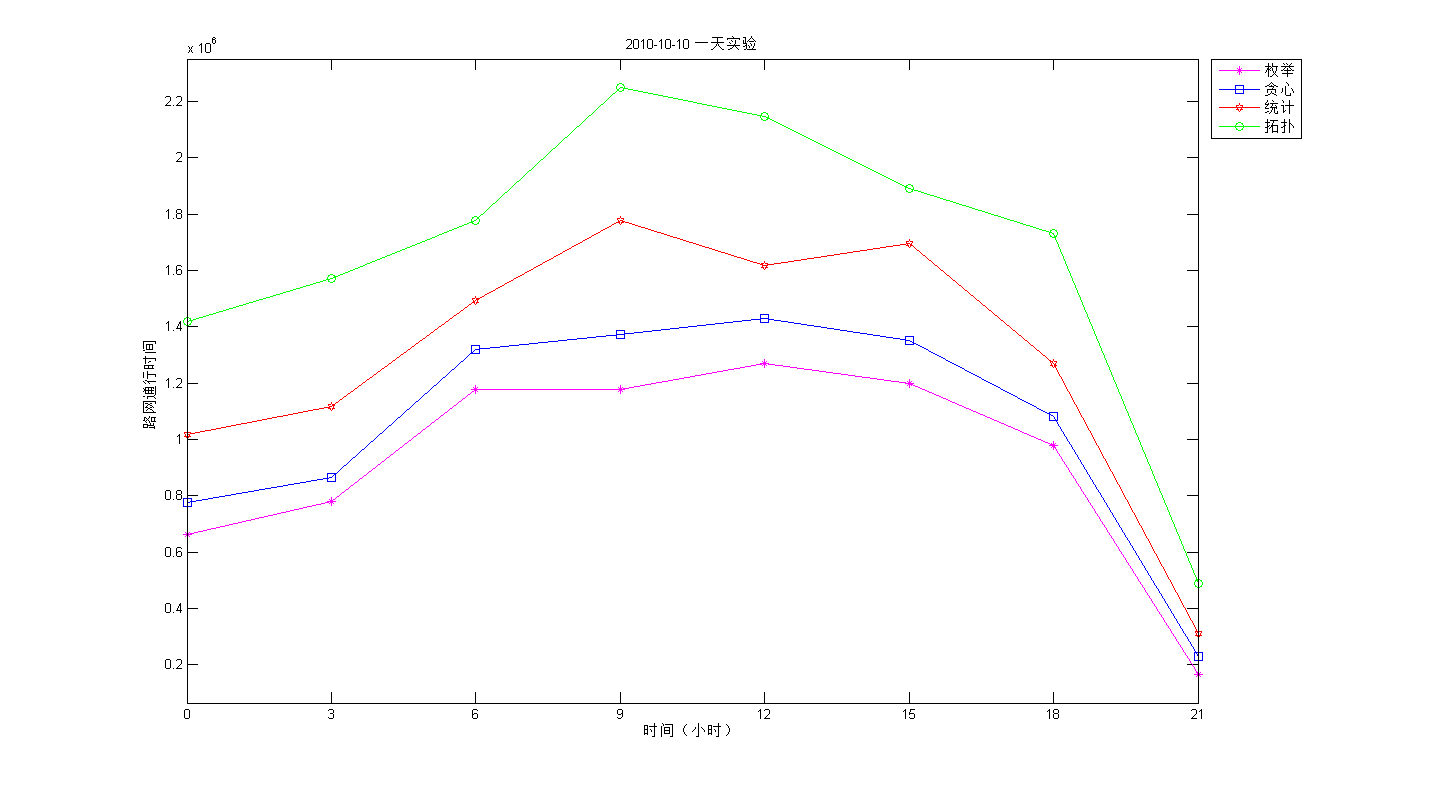
\includegraphics[width=3.0in]{picture/one_day_5}
					\caption{关键路段挖掘:以1h为区间}
					\label{fig1:a}
				\end{minipage}%
				\begin{minipage}{0.5\linewidth}
					\centering
					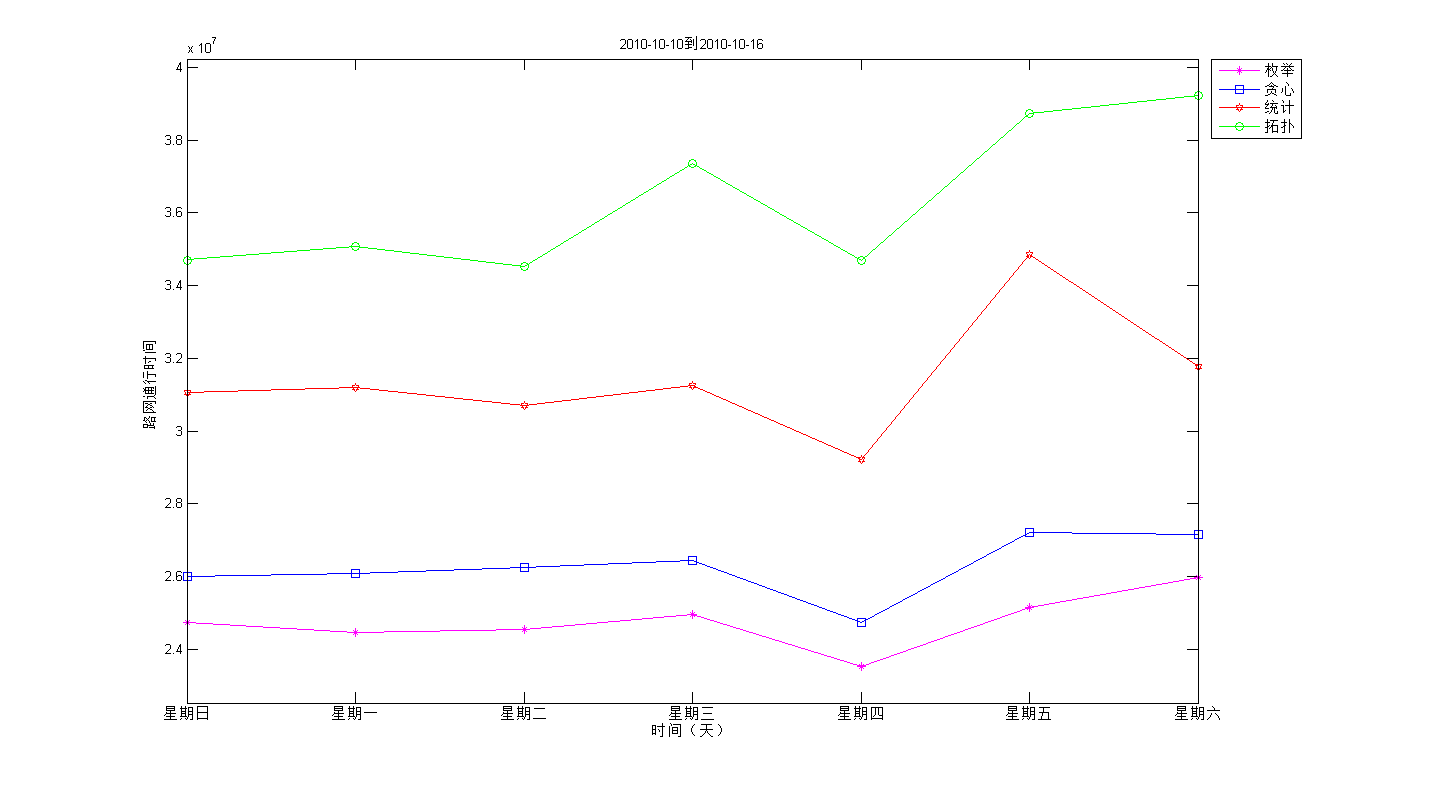
\includegraphics[width=3.0in]{picture/one_week_5}
					\caption{关键路段挖掘:以1d为区间}
					\label{fig1:b}
				\end{minipage}
				\end{figure}

				表\ref{tab:5}给出了不同方法求得的路网通行效率。表格中的数值是$L(\bm{y})$的绝对值(路网整体通行时间),可以看出贪心算法最接近最优解,而且误差在可接受范围内。

				\begin{table}[h]
				\centering
				\begin{tabular}{|c|c|c|c|c|}
				\hline
				\hline
				   &   枚举 &   贪心 &   统计 &   拓扑 \\
				\hline
				  一天 &  926030.06 & 1053575.26 & 1287439.55 & 1660243.55 \\
				\hline
				  一周 &  21674024.80 & 22989458.02 & 27510044.42 & 31790488.20 \\
				\hline
				\end{tabular}
				\caption{算法结果集}
				\label{tab:5}
				\end{table} 



				图\ref{fig2}给出了关键路段在路网中的分布图,图\ref{fig2}$(a)$是基于贪心算法求解的关键路段集合,图\ref{fig2}$(b)$是基于高速公路统计方法获得的路段集合。图\ref{fig2}$(c)$是基于枚举所得的最优解集,图\ref{fig2}$(d)$是基于路网拓扑结构选取的关键路段集合。对比图\ref{fig2}$(a)$和图\ref{fig2}$(b)$可以发现,直观上重要的点(承载流量较大的路段,事故多发路段等)并不一定在路网中属于关键路段集合,关键路段集合需要经过计算才能求出;直接枚举的路段集合与贪心算法求得的路段集合十分接近,平均有80\%以上的相似度,而统计和度中心性方法求得的关键路段和枚举方法差距较大。

						%插入图片
				%\10个收费站的情况下
				\begin{figure}
				%\begin{tabular}{cc}   
				\begin{minipage}{0.48\linewidth}
				  \centerline{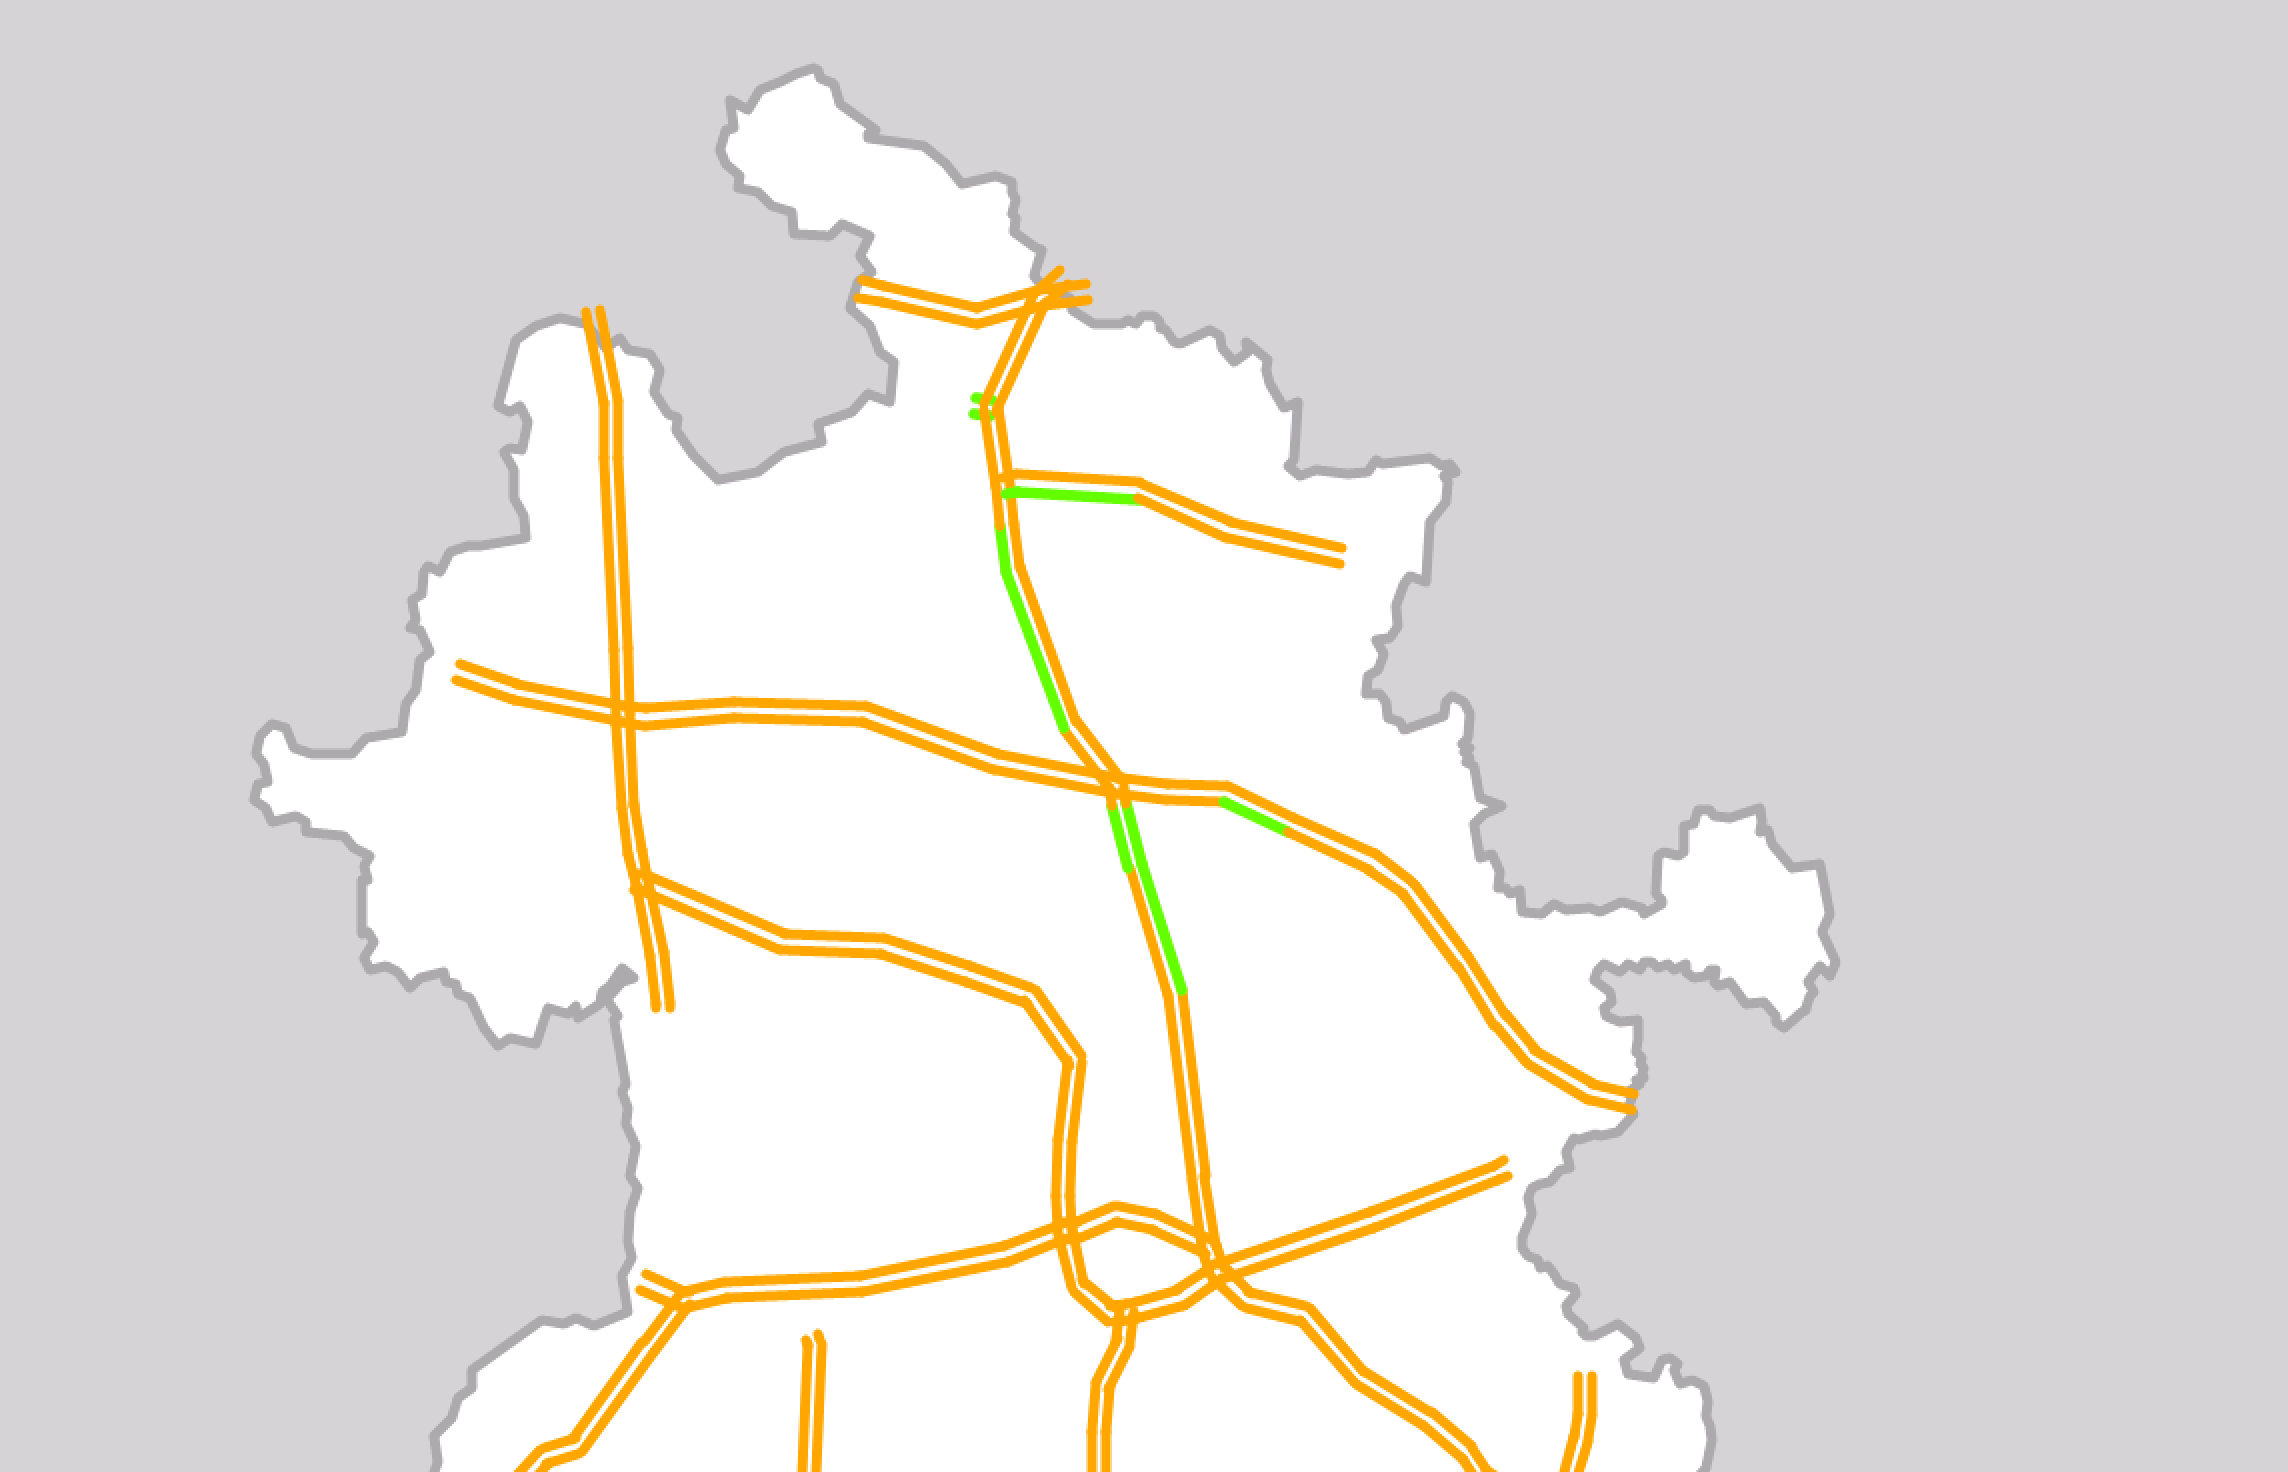
\includegraphics[width=3.0in]{picture/tanxin}}
				  \centerline{(a) 贪心算法关键路段}
				\end{minipage}
				\hfill
				\begin{minipage}{.48\linewidth}
				  \centerline{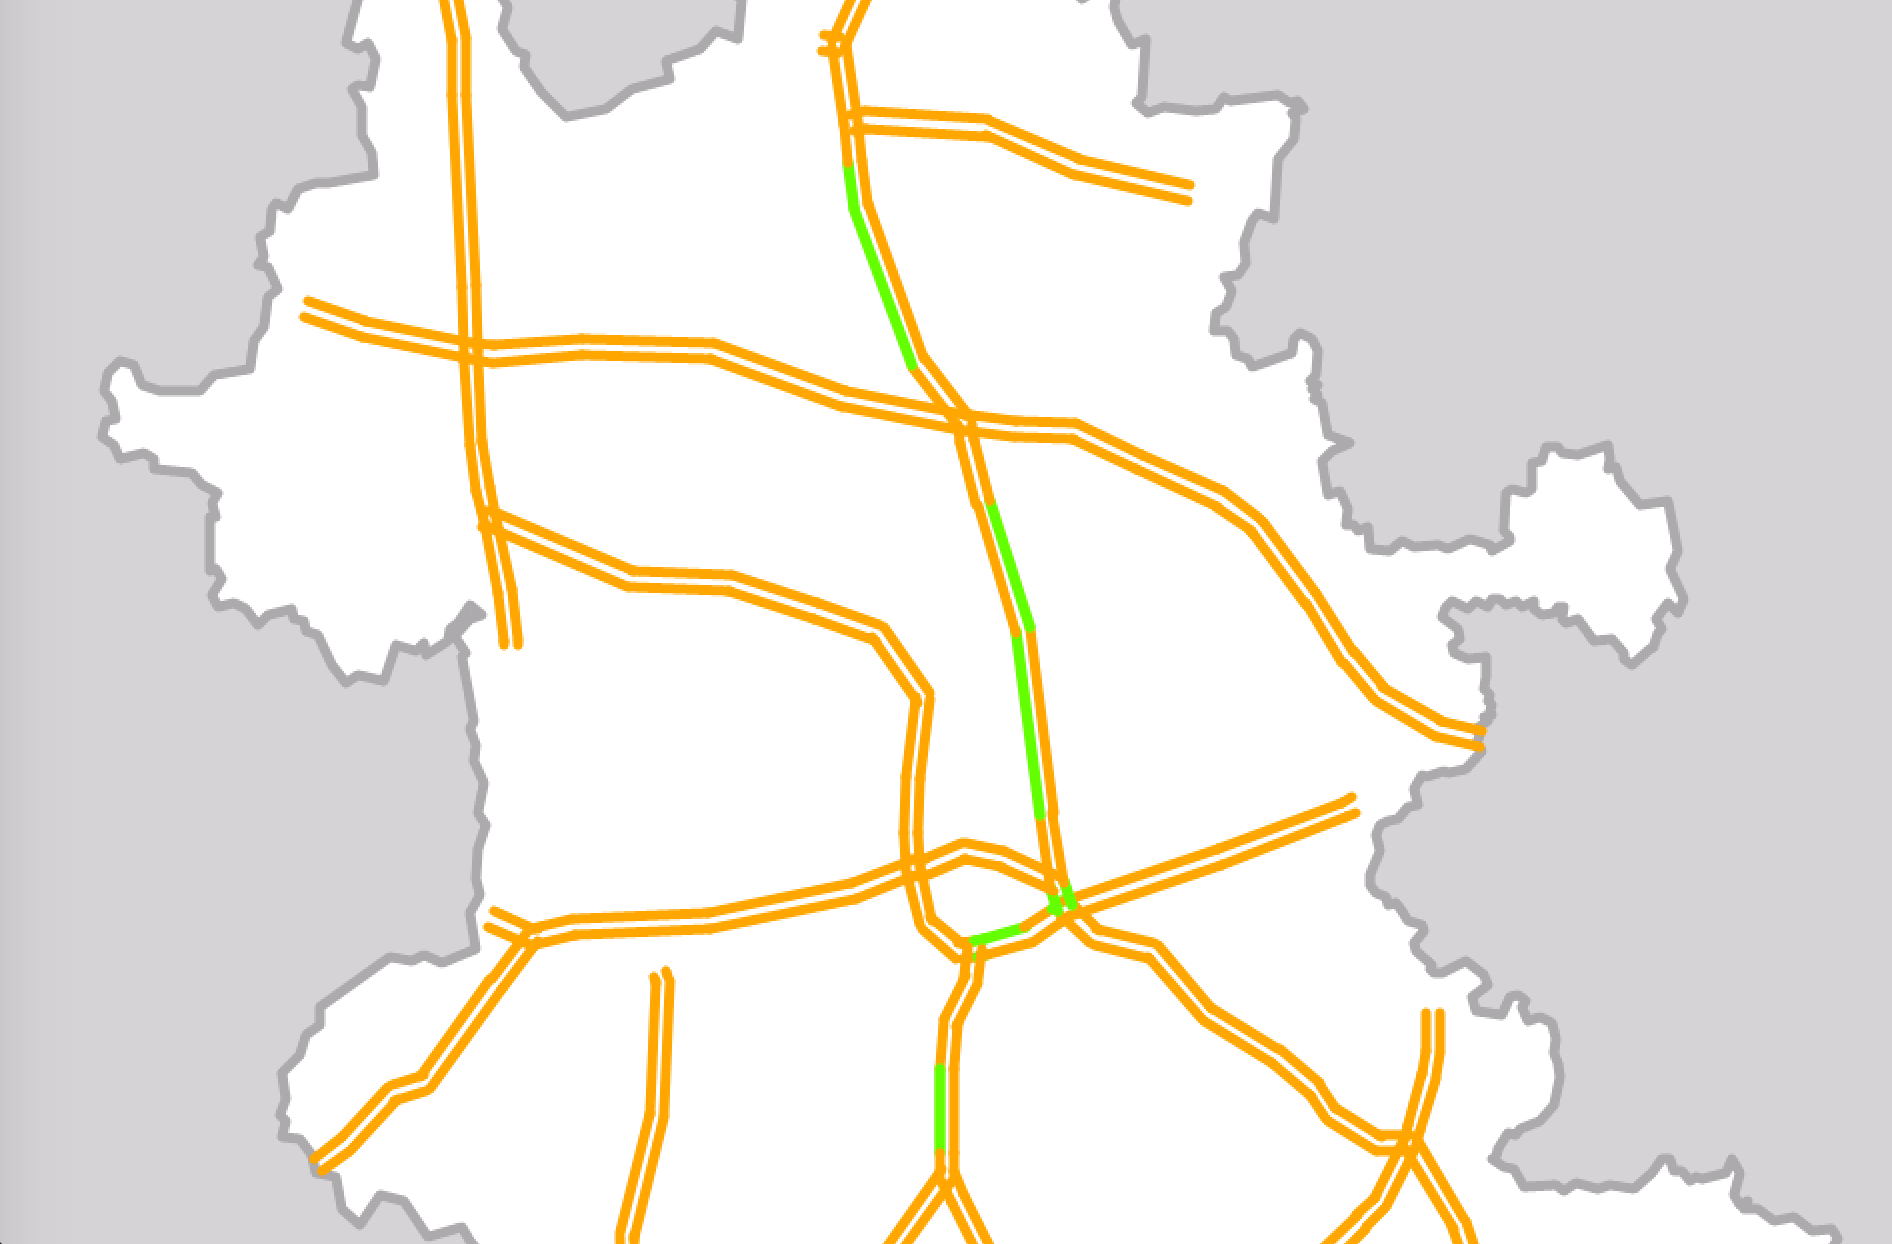
\includegraphics[width=3.0in]{picture/hotsection}}
				  \centerline{(b) 统计获得关键路段}
				\end{minipage}
				\vfill
				\begin{minipage}{0.48\linewidth}
				  \centerline{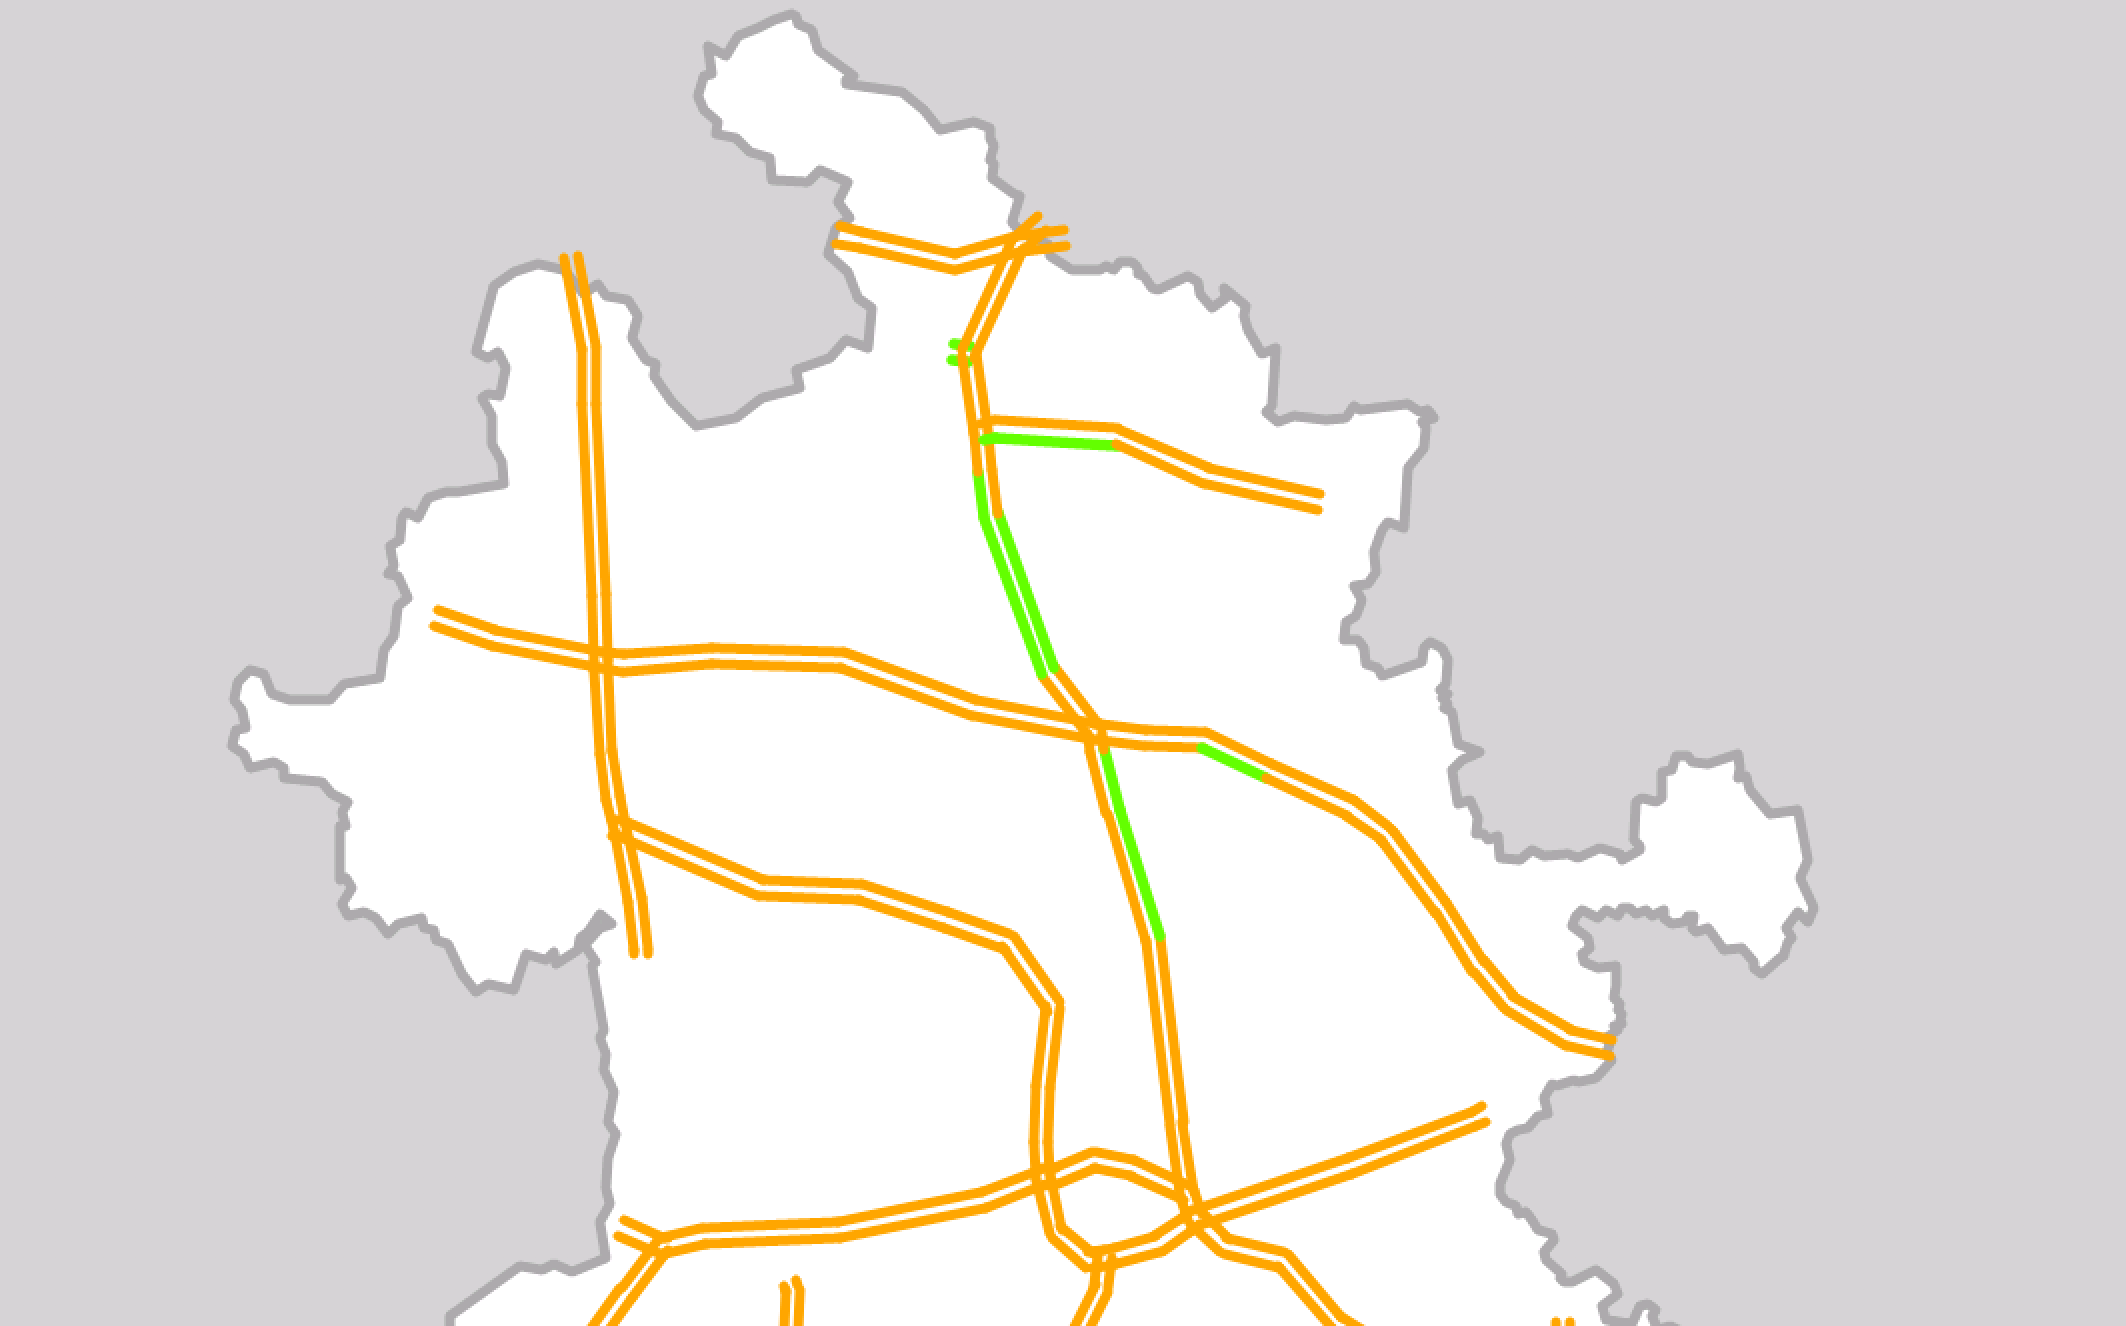
\includegraphics[width=3.0in]{picture/meiju}}
				  \centerline{(c) 枚举获得最优解}
				\end{minipage}
				\hfill
				\begin{minipage}{0.48\linewidth}
				  \centerline{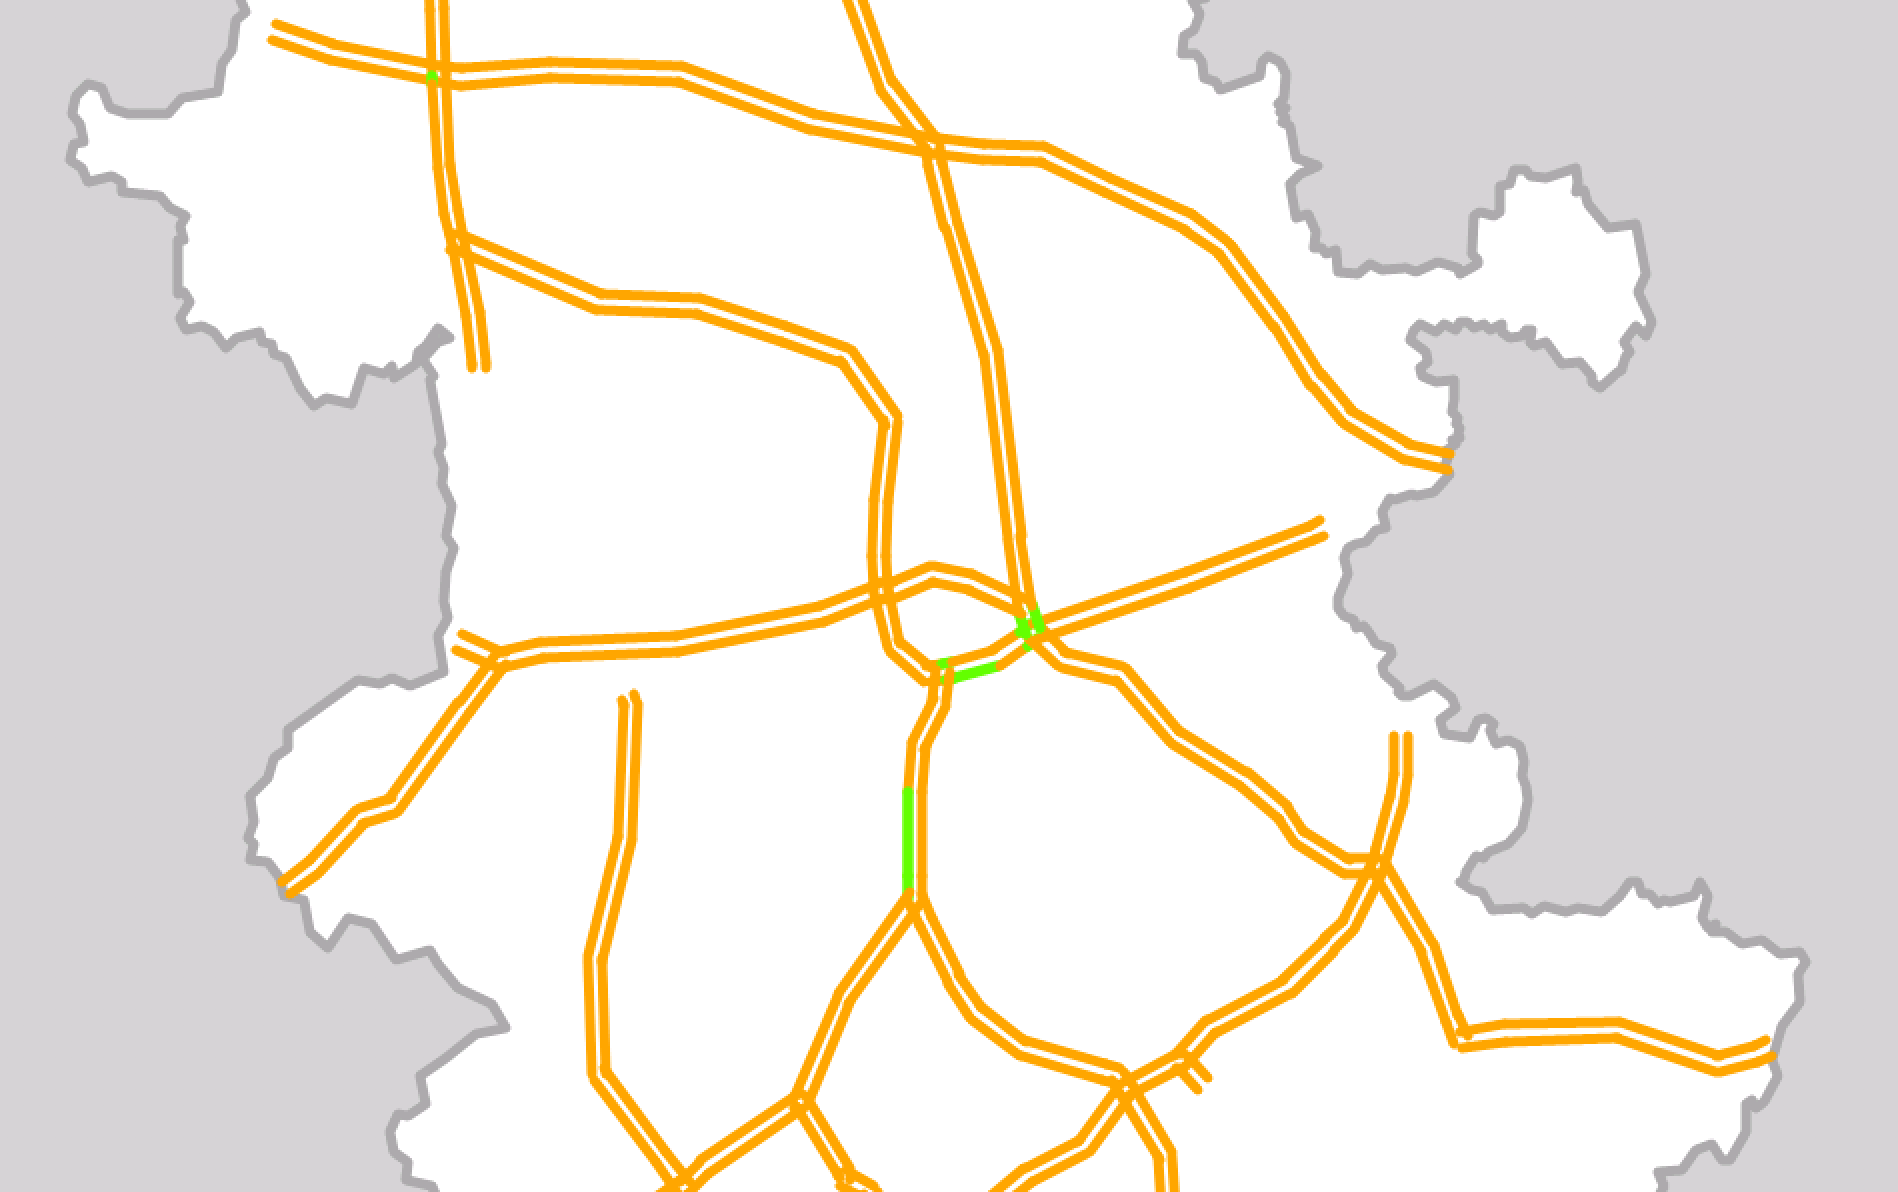
\includegraphics[width=3.0in]{picture/degree}}
				  \centerline{(d) 基于拓扑结构的关键路段}
				\end{minipage}
				%\end{tabular}
				\caption{不同方法求得的关键路段结果图}
				\label{fig2}
				\end{figure}

				在实验过程中,我们还发现当时间区间缩短到1h时,高速公路网络中的关键路段具有随着时间和流量变化而变化的特性。图\ref{duibi1}是凌晨3点时的高速公路关键路段集合,图\ref{duibi2}是早上九点时的高速公路关键路段集合。这一发现证明了高速公路的关键路段具有动态变化特性,即高速公路的关键路段不是一成不变的,而是会随着整个路网的流量的变化而变化。


				\begin{figure}[h]
				\begin{minipage}{0.5\linewidth}
					\centering
					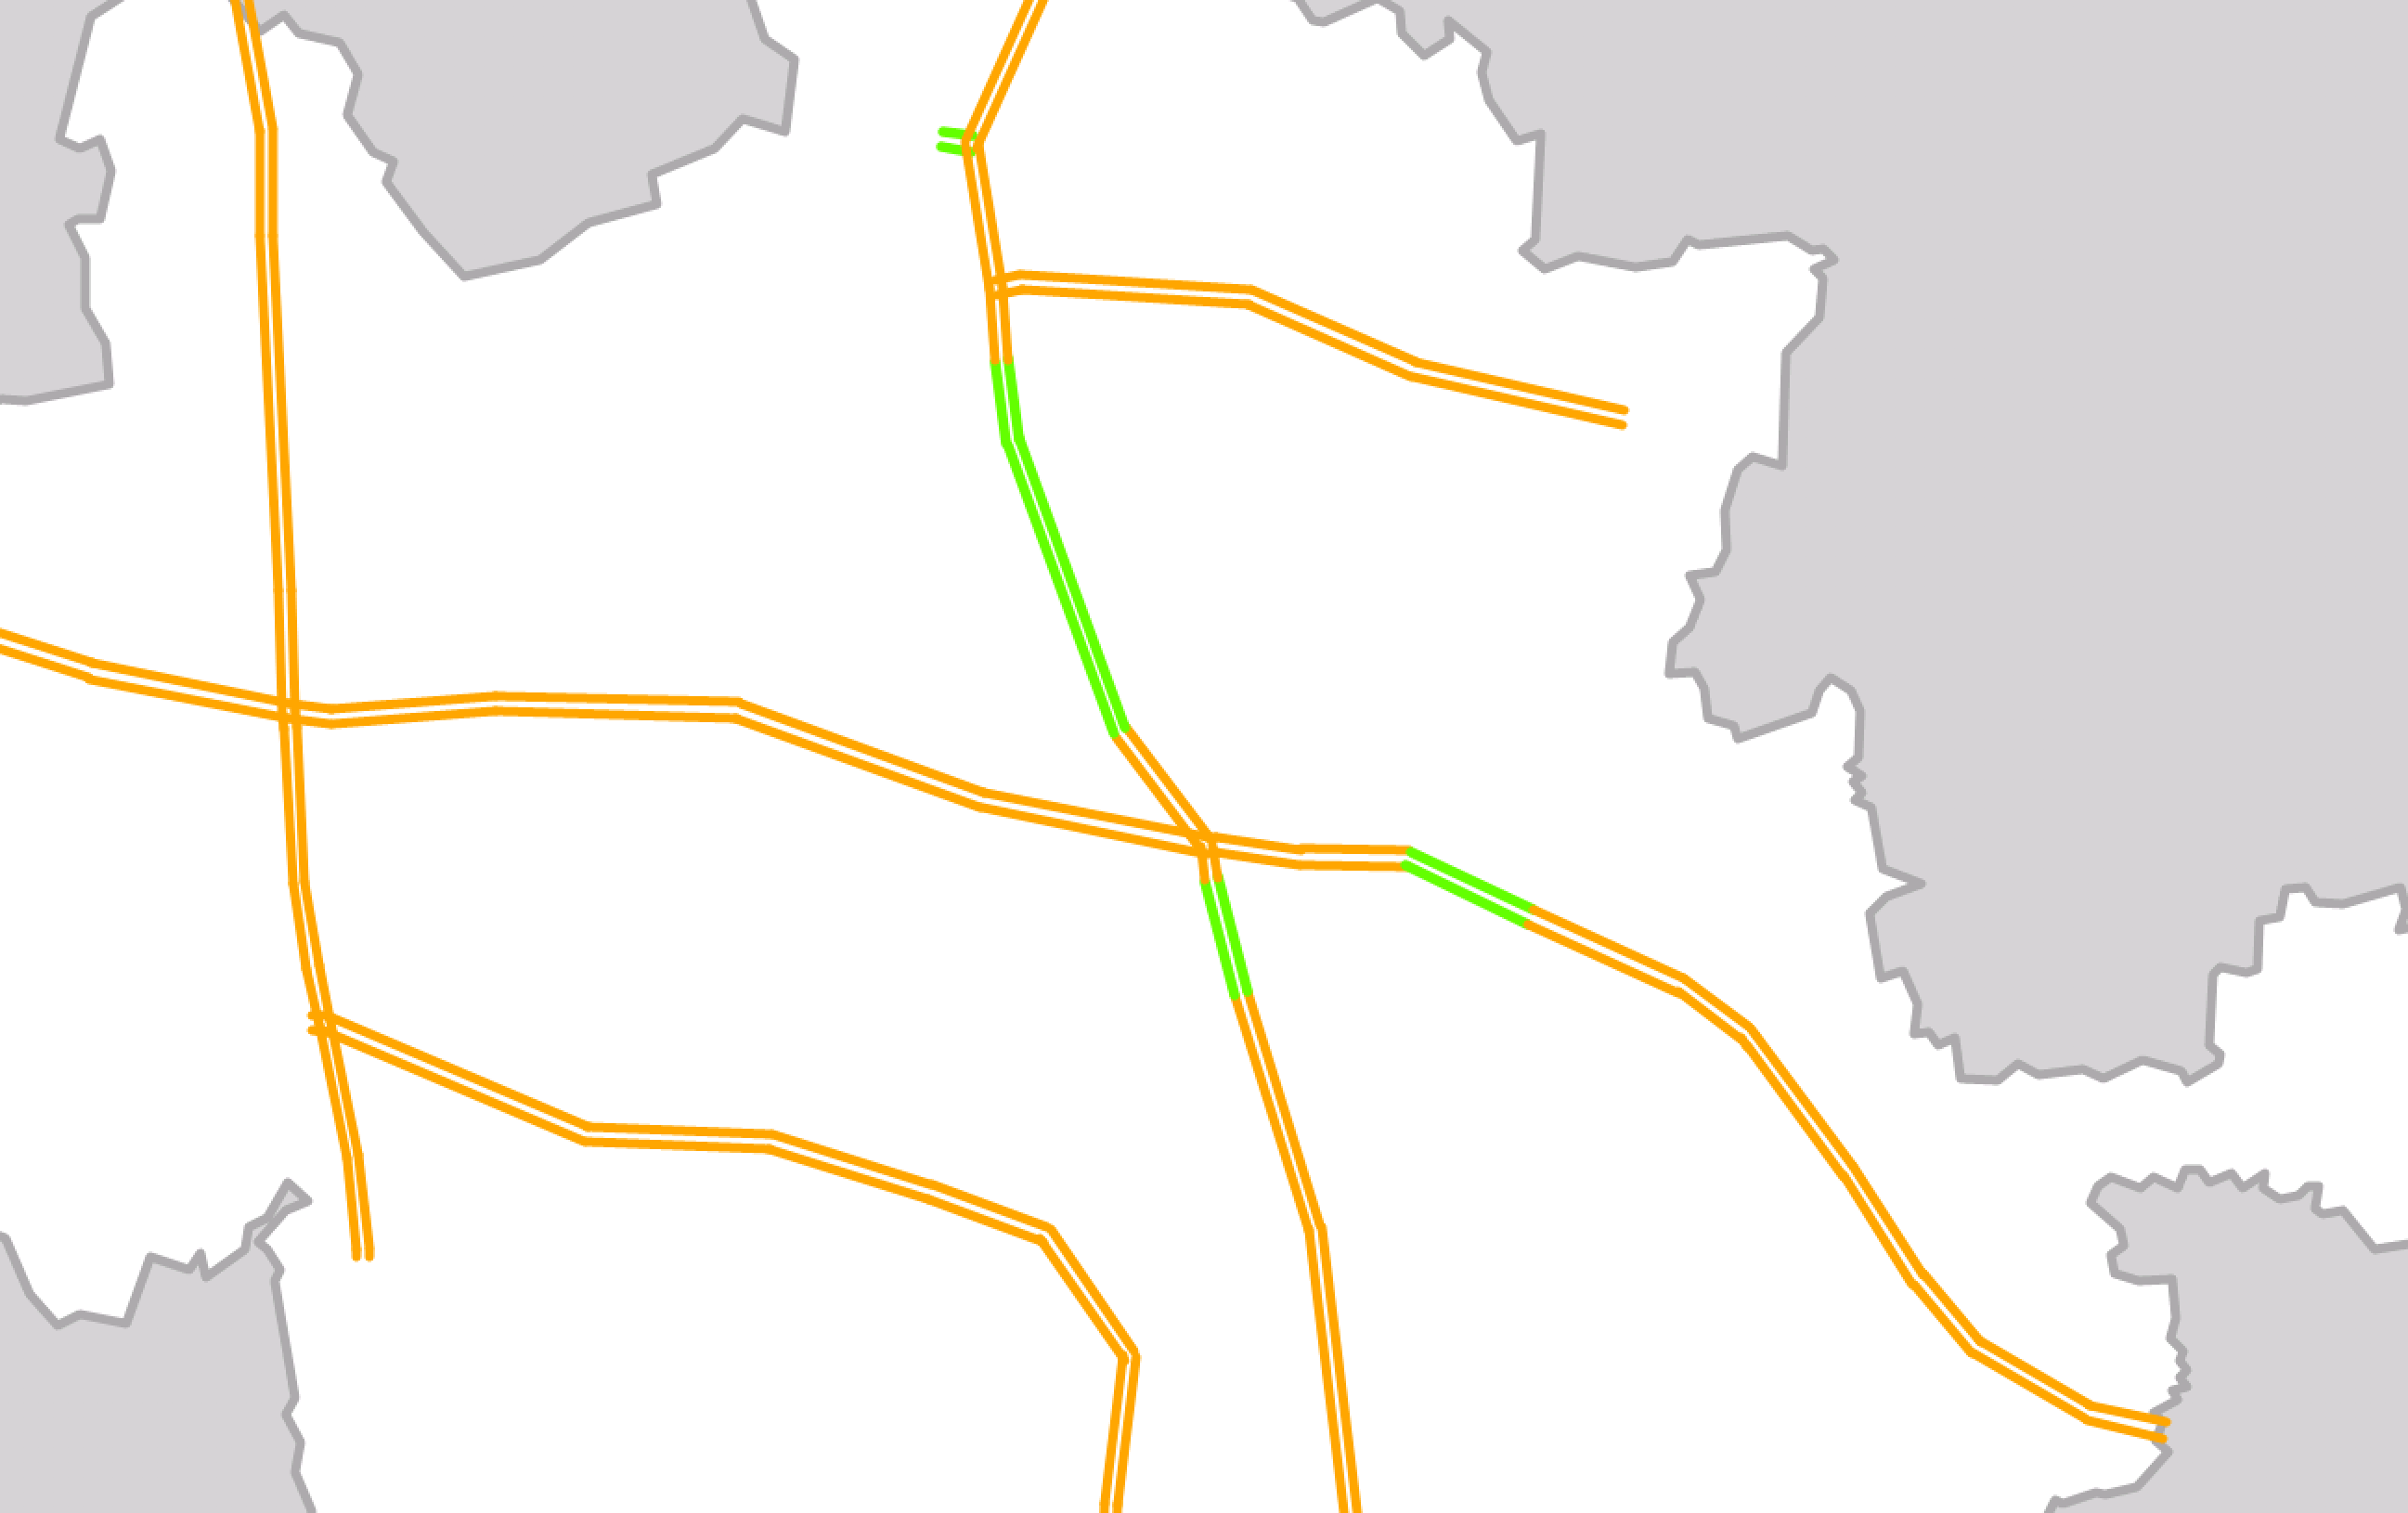
\includegraphics[width=3.0in]{picture/duibi1}
					\caption{关键路段挖掘:03:00}
					\label{duibi1}
				\end{minipage}%
				\begin{minipage}{0.5\linewidth}
					\centering
					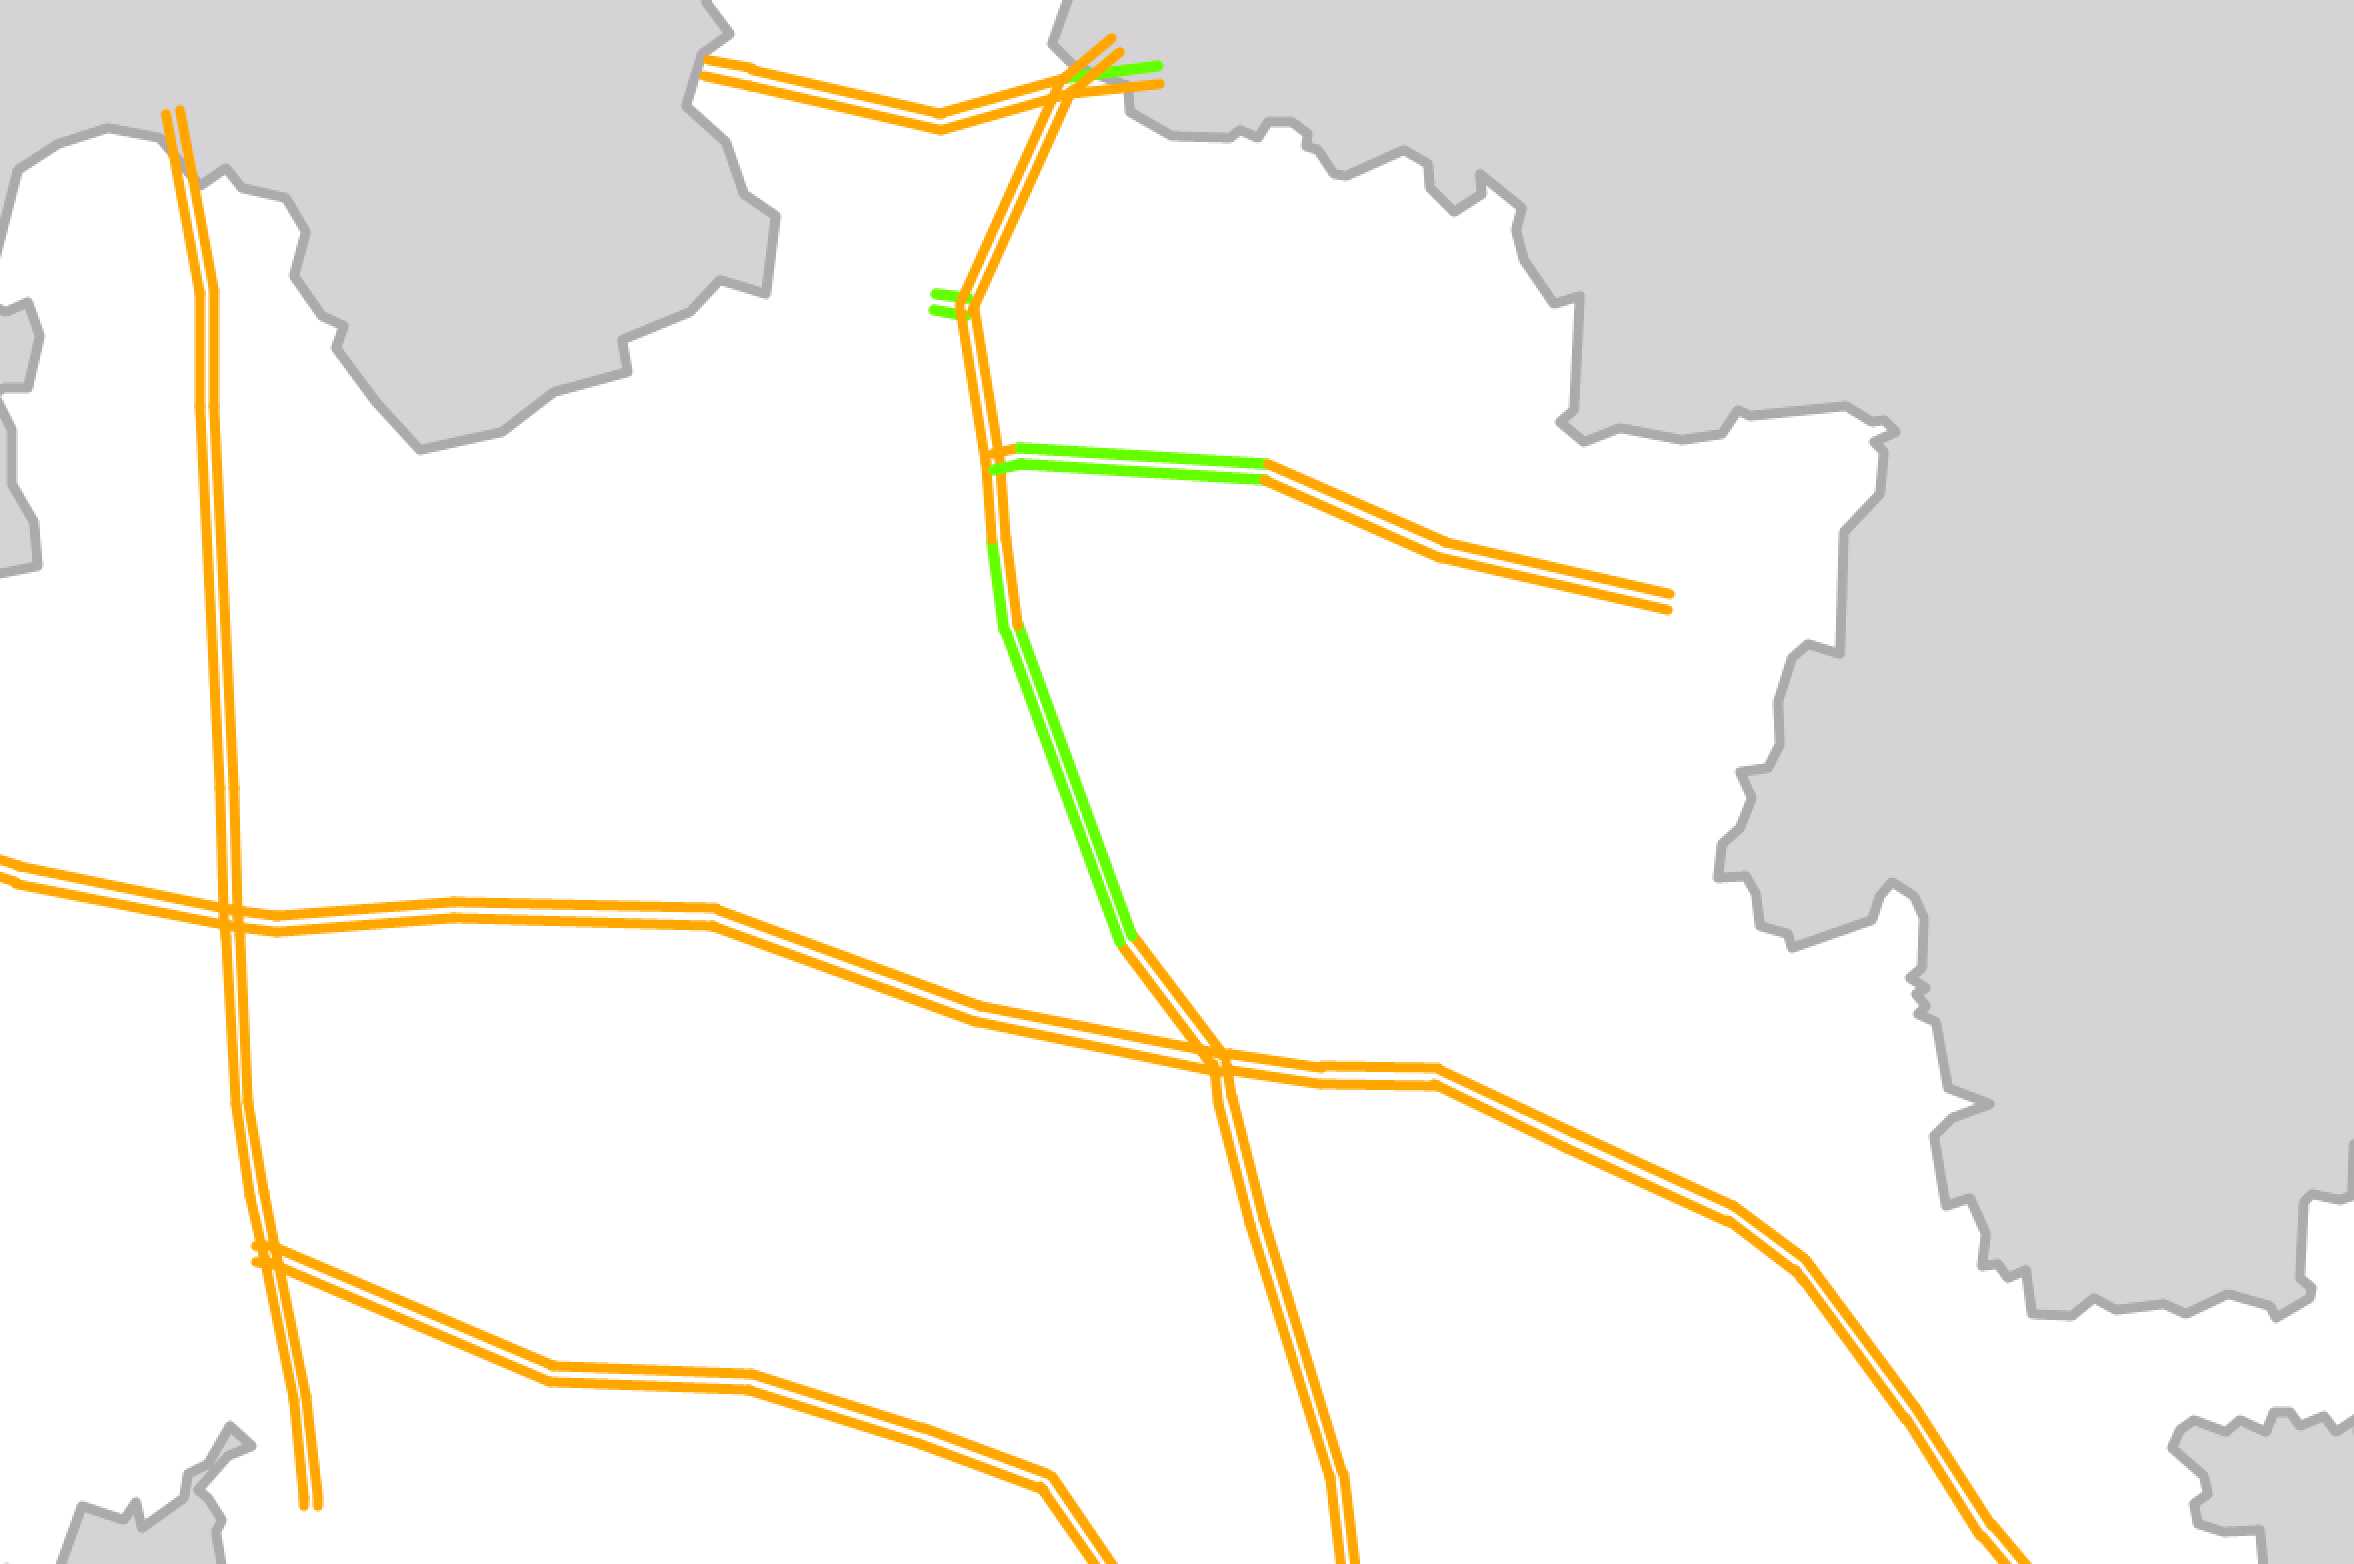
\includegraphics[width=3.0in]{picture/duibi2}
					\caption{关键路段挖掘:09:00}
					\label{duibi2}
				\end{minipage}
				\end{figure}

			\subsection{时间分析}
				基于暴力枚举方法的时间复杂度:$O({n^B}*{2^n})$

				基于贪心算法的时间复杂度:$O(n*B*{2^n})$

				基于统计路段重要性方法的时间复杂度:$O(n*\log (n))$

				基于路网拓扑结构方法的时间复杂度:$O(n*\log (n))$

				实验时间如表\ref{table1}所示,第一行代表实验的方法,第一列代表实验数据的范围,表格内的数值是实验的平均运行时间。

				\begin{table}[h]
				\centering
				\begin{tabular}{|c|c|c|c|c|}
				\hline
				\hline
				   &   枚举 &   贪心 &   统计 &   拓扑 \\
				\hline
				  一小时 &   1day &   30min &   1min &   1min \\
				\hline
				  一天 &   6day &   2h &   2min &   1min \\
				\hline
				  一周 &   7day &   3h &   5min &   1min \\
				\hline
				  一月 &   7day &   3h &   8min &   1min \\
				\hline
				\end{tabular}
				\caption{不同算法的运行时间}
				\label{table1}
				\end{table} 

				由表格可以看出,在以一个省为数据集的基础上,枚举方法已经处于一种较大的时间复杂度;贪心算法在一定程度上解决了算法过慢的情况,并且在精度上有一定的保证,可以应用于静态路网关键路段识别问题,但是对于动态实时应用仍旧不够;基于统计领域的路段重要性排序方法、基于路网拓扑结构的关键路段挖掘方法虽然在时间上效率较高,但是在精度上达不到要求。一周和一月的时间差距较小的原因是:对数据进行预处理,O-D相同的用户被归为一类。在时间区段增大到一定程度时,O-D类数量不再增加,算法运行时间增长较小。

		\section{本章小结}
			本章提出了一种面向高速公路网络的关键路段挖掘模型,同目前高速公路关键路段已有的挖掘方法相比,该方法的优势是结合高速公路的特性,考虑高速公路上的车流流量、路段事故率,从宏观角度提出一个整体的优化模型。针对上述模型,本章分析证明了模型的次模性,并给出基于贪心方法的关键路段挖掘方法。特别的,本文通过枚举方法,在较低的时间效率下计算高速公路中的最优解。结果表明该模型的贪心算法解可以很好地逼近真实解,并且在时间复杂度上有了规模性的优化,证明了贪心算法的可行性。然而,即使贪心算法可以在一定规模上优化整体的时间复杂度,并且可以在实际应用中运行良好,但是这是基于目前的研究目标是静态关键路段挖掘,同时高速公路也只有部分路段产生过断流等重大事故的情况下达成的。当任务环境更为复杂时(扩大到全国高速公路网络),当管理者需要更加迅速得到实时反馈的时候,上述方法受到算法计算规模的约束,无法达到预期的效果。下一章将针对高速公路的网络特性,给出相应的解决手段。





			

	% vim:ts=4:sw=4
% Copyright (c) 2014 Casper Ti. Vector
% Public domain.

\chapter{基于社群划分的关键路段识别方法}
	本章主要分四小节。第一节讲述了模型的性质,分析了贪心算法的不足;第二节给出了基于社群划分的关键路段挖掘方法模型;第三节是实验结果;第四节总结了本章内容。
	\section{引言}
		上一章介绍了面向高速公路的关键路段挖掘模型,并给出了贪心算法。然而根据模型的定义,就算进行简化,认为关键路段已经选出,计算对关键路段进行维护之后的整体网络通行效率也需要$2^n$的时间复杂度。贪心算法的实际时间复杂度是
		$$O(B*n*2^t)$$
		式中B表示关键路段数量,n表示网络中路段的数量,t表示网络中可能出现损毁的路段数量。虽然在实际应用中,高速公路中路段规模不大$(O(10^3))$,大部分路段的损毁概率是0,贪心算法对于静态高速公路中的关键路段挖掘可适用性高,但是贪心算法的时间复杂度仍旧属于指数级别,当高速公路网络规模变大后,复杂度指数上升,对于有实时性要求的动态关键路段挖掘方法并不适用。本节给出基于复杂网络社群划分的关键路段挖掘方法。

		模型需要从输入的代表关键路段的离散0-1向量$\bm{y}$,求得高速公路网络通行效率的期望。这种输入为整数或整数向量,并且内部具有概率事件的问题,属于随机整数规划问题。在数学优化领域,随机规划是一个涉及不确定性优化问题的框架。比如说两阶段线性规划。决策者在第一阶段采取一些行动,之后发生随机事件影响第一阶段决策的结果。不断调整第一阶段的决策,使得整体期望收益达到最大。

		现有的随机整数规划问题大都是基于班德斯分解方法(Benders Decomposition)进行研究,然而班德斯优化方法要求有两层模型,且两层模型之间互不影响。本研究中,第一层的决策变量$\bm{y}$会直接影响到第二层里面的路网拓扑结构概率,对于这种相互依赖的随机规划问题,现有的研究没有找到适用的优化方法。

	\section{问题定义}


		\subsection{问题定义}

			高速公路网络除具有绝大多数复杂网络的特征外,作为空间网络还具有不同于抽象网络的特性,这些特性决定了高速公路网络的拓扑性质。具体可以归纳为:高速公路交通网络的节点存在于真实物理空间,高速公路网络中的边是一种实体联接,具有明确的空间意义。高速路网中的边与抽象网络中的边不同,高速公路交通网络中节点的边权与交通距离直接相关,这一特性直接影响着高速公路网络出现小世界行为的可能性\parencite{ysk2017qx};高速公路交通网络中单一节点所能联接的边的数目受到物理空间的限制,这种限制会影响到网络的复杂程度。

				在高速公路项目研究中,我们发现低跳数的用户占大多数。如图$\ref{fig4}$,可以发现在高速公路中,低跳数的车辆占了大多数,10跳以下的车辆占所有车辆总数的90\%以上。再结合高速公路的异质性,复杂网络的社群性,我们认为高速公路网络应该也具备社群性质,即存在一个个社群,这些社群各自包含一些收费站和高速公路路段,高速公路中的车辆大都从社区内部的节点出发,在同一个社区的另一个节点驶离。社区之间的车辆交流尽量小。

				\begin{figure}[h]
				\centering
						\begin{minipage}{0.8\linewidth}
							\centering
							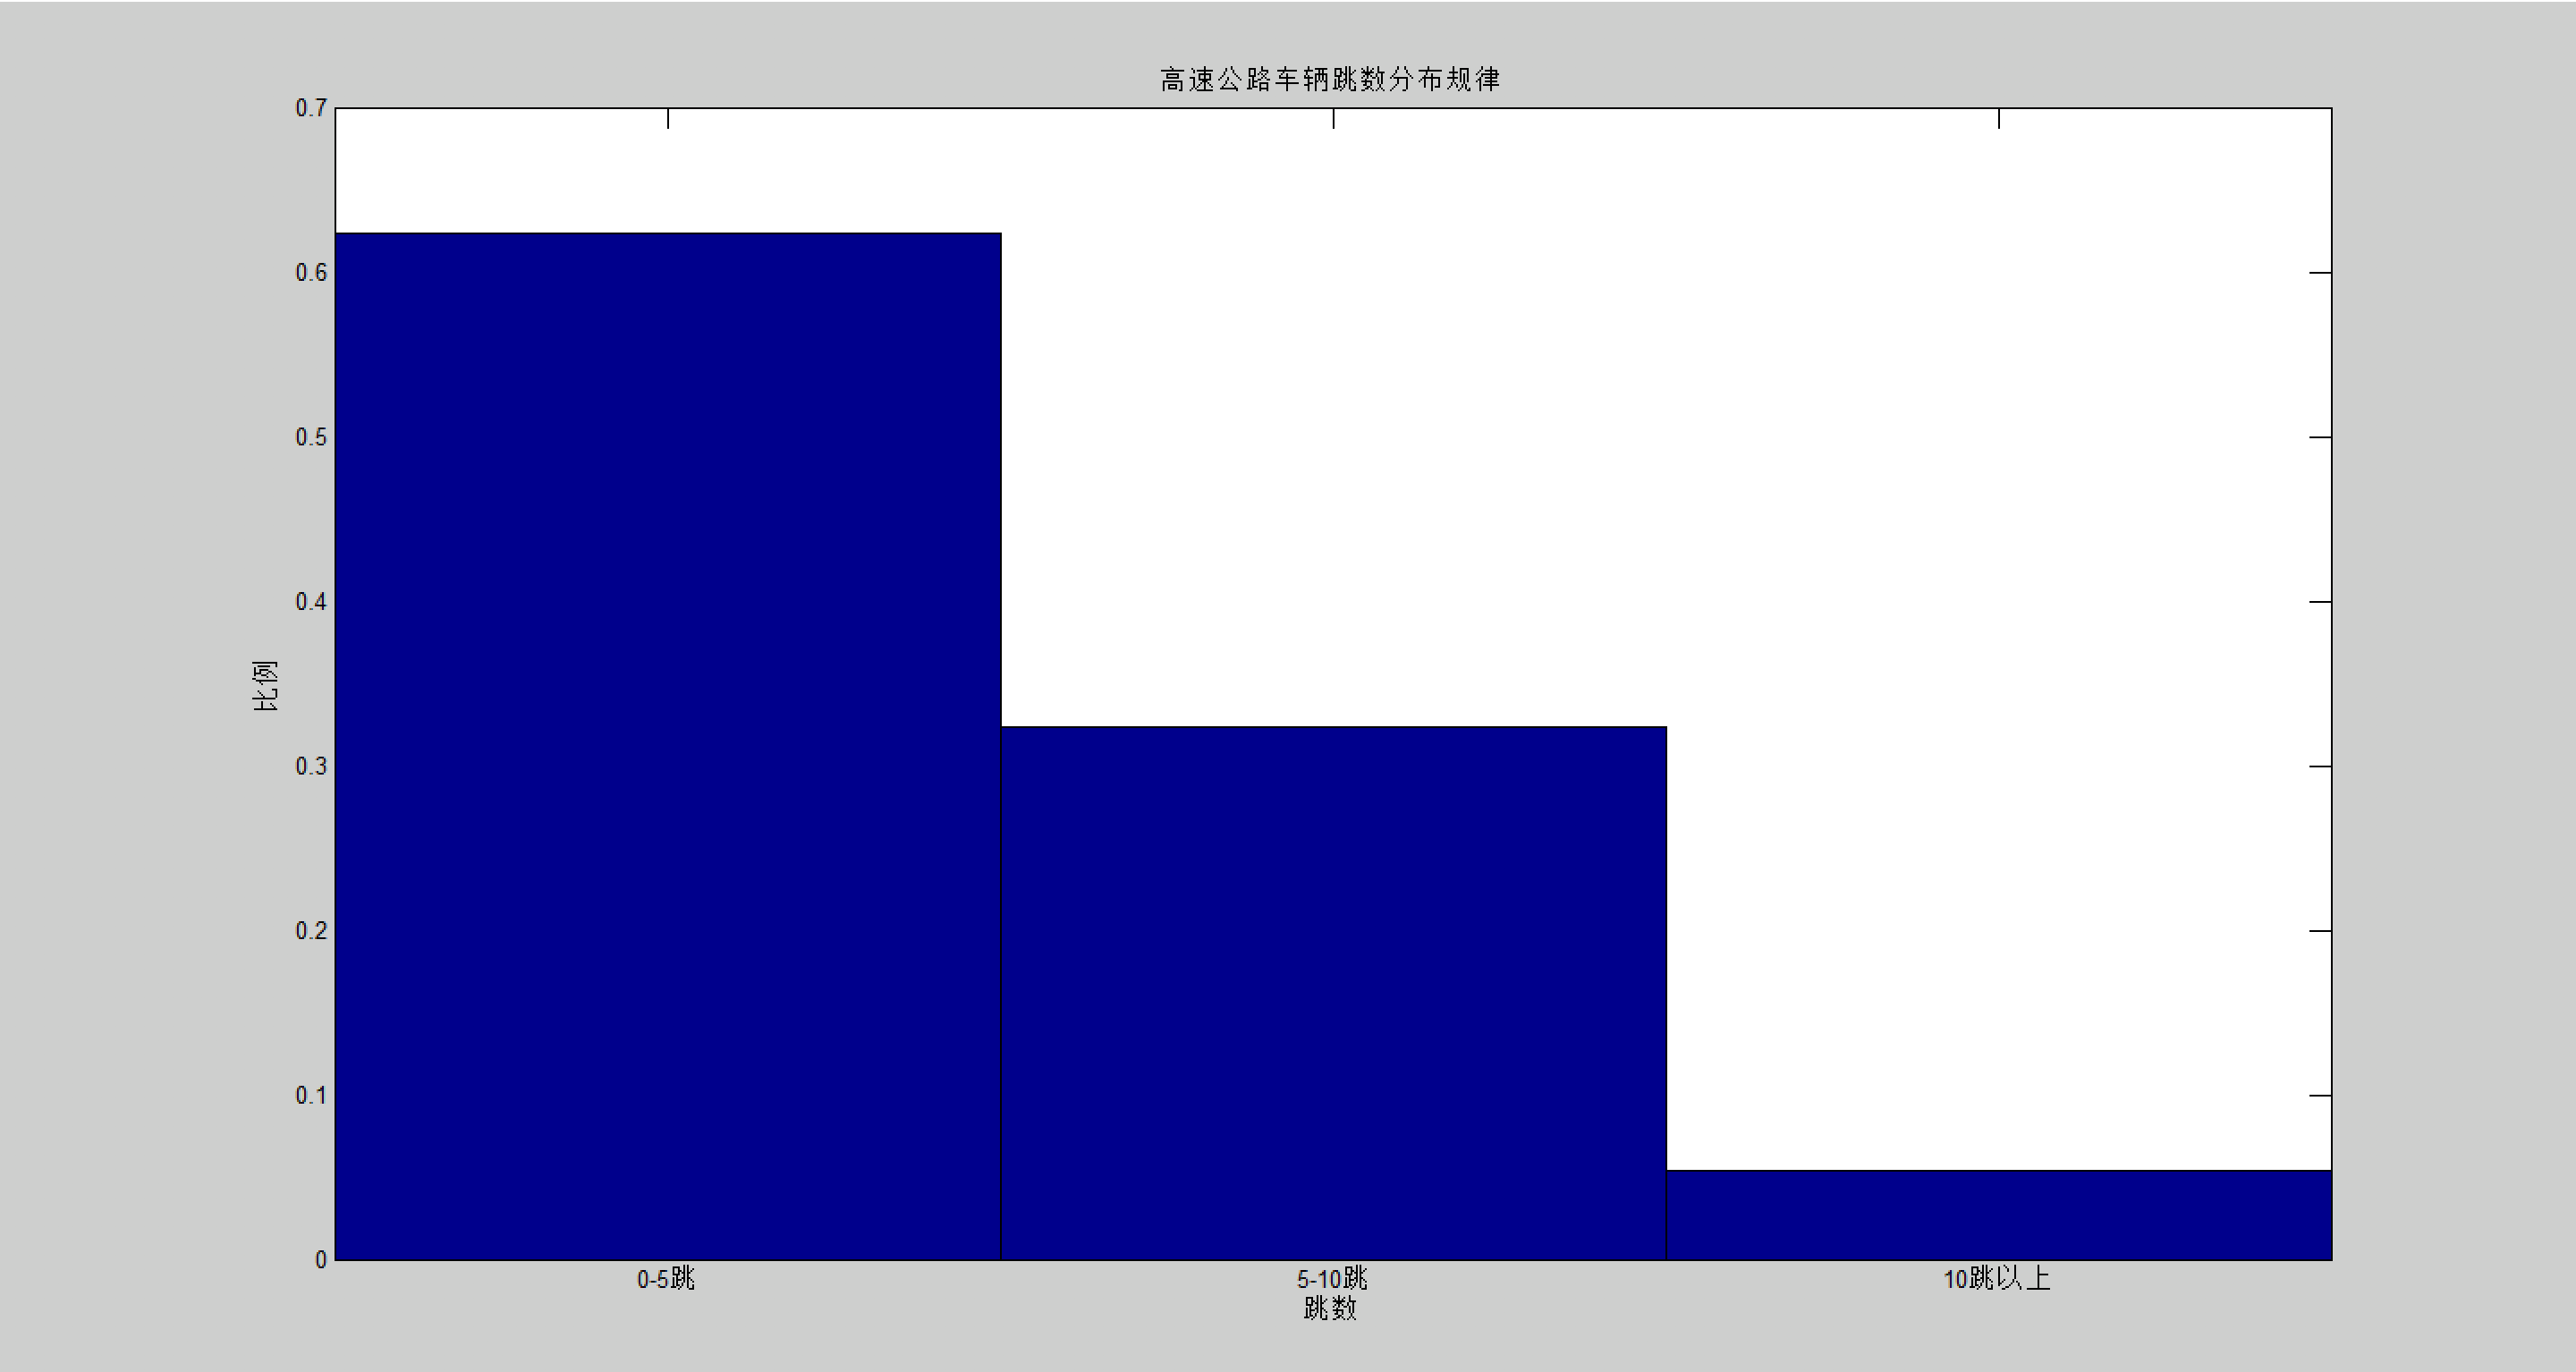
\includegraphics[width=4.4in]{picture/tiaoshu}
							\caption{高速公路车辆跳数分布图}
							\label{fig4}
						\end{minipage}%\
				\end{figure}

				为此,抽取某一天的高速公路O-D数据,将有O-D交流的收费站之间连线,流量越多,线的颜色越深,流量越少,线的颜色越浅。如图\ref{fig5},可以较直观的看出高速公路的社群特性。

				\begin{figure}[h]
				\centering
						\begin{minipage}{0.8\linewidth}
							\centering
							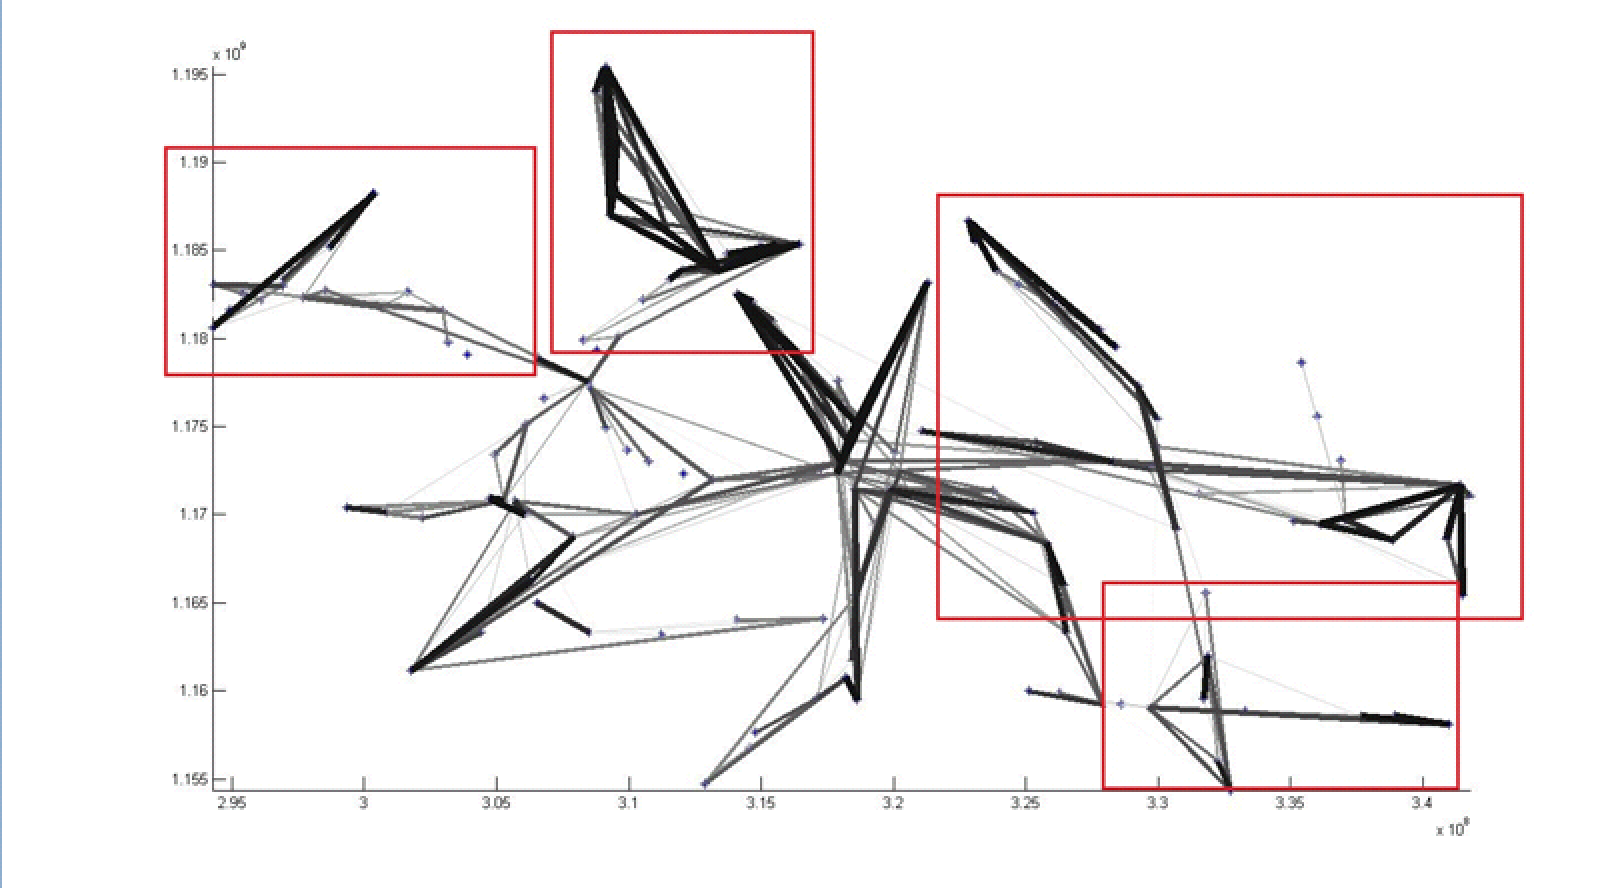
\includegraphics[width=4.4in]{picture/shequntexing}
							\caption{高速公路社群特性}
							\label{fig5}
						\end{minipage}%\
				\end{figure}
			%查重

				高速公路社群划分的目的是将整个高速公路拓扑结构分成一个个社区,使得社区内部交流尽量多,社区之间的交流尽量少,最终在各自社群分别计算关键路段,分治计算,最后进行合并,达到优化算法效率的目的。在此引入基于模块性优化的社区划分方法。

				复杂网络具有社群特性,高速公路属于复杂网络的一种。给定高速公路有向图$G=\{V,E\}$,其中V代表收费站(节点)的集合;E表示边的集合。定义社群$c=\{v_1,v_2,...v_m\}$,其中$v_i$是网络中的节点,即收费站或者交叉路口;社群集合$C=\{c_1,c_2,...c_u\}$;其中$v_i \in V$,${c_i}\bigcap {{c_j}}  = \emptyset$,$\sum\limits_{i = 1}^u {\sum\limits_{v \in {c_i}} v  = V}$。

				基于高速公路社群划分的关键路段挖掘算法主要采用分治思想,将一个难以直接解决的复杂问题,分割成一些规模较小的问题,逐个计算,分而治之。本文主要将路网分成一个个子路网,在子路网中分别计算关键路段,之后再用一定的方法进行合并。在此需要解决两个问题:

					1)如何分群

					2)分群求解后,如何合并

				传统的复杂网络社群划分方法中,大都是针对虚拟网络(如社交网络)进行研究。高速公路网络和虚拟网络有很大的不同。在虚拟网络中,两个点之间只要有交流,那就代表有边相连;在高速公路中,我们认为只要两个收费站有流量交流,即O-D不为0,那么这两个收费站之间就有边连接(不同于上一章的路网定义)。但是这个边和其他的复杂网络如社交网络不同,社交网络中两个节点之间的空间距离定义为1跳,但是对于物理网络来说,两个节点之间的边具有实体距离。高速公路中路段之间的影响也会根据物理距离的变化而变化,这些都是传统方法中没有考虑到的。

				2004年,Newman和Girvan\parencite{NewmanBasic}提出了一个用于刻画网络社区结构优劣的量化标准,被称作模块化函数。简单的带权模块化函数定义如下:

				\begin{equation}
				Q = \frac{1}{{2m}}\sum\limits_{ij} {[{A_{ij}} - \frac{{{k_i}{k_j}}}{{2m}}]\delta ({c_i},{c_j})}
				\label{eq4}
				\end{equation}

				式\ref{eq4}中,$A_{ij}$表示节点$i$和节点$j$之间的边权;$k_i=\sum\limits_{j} {A_{ij}}$表示所有与节点i相连的边的边权和;$c_i$是指i所属的社群编号;如果$c_i=c_j$,那么$\delta (u,v)=1$,否则等于0;$m=\frac{1}{{2}}\sum\limits_{ij} {A_{ij}}$。

				模块化函数主要用于度量社群划分结构的优劣,现有的基于模块化函数的分群算法都没有考虑高速公路的特性\parencite{WeightPretreatment},并且在高速公路网络上出现了低分辨率特性和极端退化特性\parencite{Ren2014The}。Newman提出了一种社群挖掘方法\parencite{NewmanFast}:初始的时候没个节点都是一个社群,之后进行迭代,每次迭代时都选择使目标模块函数在Q增加最大的社群进行合并。这个方法虽然在时间效率上很高,但是没有解社群划分的决极端退化特性。Guimera提出一种基于模拟退火的模块性优化方法:初始解是随机生成的社团集合,在每次迭代过程中,采用一定策略,结合当前解生成新的解集,用模块化函数Q判断解集的优劣,最后用模拟退火中的Metropolis准则来决定是否采用该解。这个方法虽然在一定程度上解决了极端退化特性,但是他有一个很严重的问题,在相通的输入集合上,生成的最终结果往往不同,不符合稳定性要求,而且时间复杂度大,求解效率低。Blondel\parencite{TuihuoEfficency}提出快速模块优化方法,他认为首先在局部使用局部模块化函数f获得局部社团,然后再对这些局部社团作为一种超级节点,再进行合并,不断迭代,直到模块化函数Q不再增加为止。这个聚类方法存在聚类社团过大的情况,不符合本文中缩小节点量级,优化算法时间复杂度的目的。针对现有研究的不足,结合高速公路的路网特性,在此提出一种新的面向高速公路的社群划分模型。
		\subsection{模型定义}

				首先定义模块化函数Q:

				\begin{equation}
				\vartriangle Q = [\frac{{\sum_{in} C  + 2{k_{i,in}}}}{{2m}} - {(\frac{{\sum_{tot} C  + {k_i}}}{{2m}})^2}] - [\frac{{\sum_{in} C }}{{2m}} - {(\frac{{\sum_{tot} C }}{{2m}})^2} - {(\frac{{{k_i}}}{{2m}})^2}] - L(i)
				\label{eq5}
				\end{equation}

				公式\ref{eq5}用于判断当节点从一个社区转移到另一个社群的时候,整体路网的社群化结构的变化。根据变化的大小决定节点的社群归属。式中,$\sum_{in} C$表示社群$C$内部的所有边的权重和;$\sum_{tot} C$表示所有与社群$C$中的节点相连的边的权重和;$k_{i,in}$表示$i$到$C$中所有节点之间的连线的权重和;$k_i$表示所有和节点i直接相连的边的权重和;m是路网中所有边的权重之和;$L(i)$是模型罚项,代表i转移社群后,不同社区之间交通流的变化。

				$L(i)$:

				\begin{equation}
				L(i)=\frac{{{k_{i,{c_1}}} - {k_{i,{c_2}}}}}{{{k_{{c_1},{c_2}}}}}
				\label{eq6}
				\end{equation}

				式\ref{eq6}中,${k_{i,{c_1}}}$表示路段i流向社群$c_1$的流量,$k_{i,{c_2}}$代表路段i流向社群$c_2$的流量,${{{k_{{c_1},{c_2}}}}}$表示社群$c_1$,$c_2$中所有节点之间的流量和。

				本文提出的模型中,边的权重不止与两个节点之间的流量有关,还与两个节点之间的物理距离有关。和传统复杂网络不同,节点之间的距离不再由节点之间的最短跳数决定,而是由节点之间的最短物理距离$L$决定:
				\begin{equation}
				L_{ij}=\sum\limits_{e \in E_{ij}} {e}
				\label{eq10}
				\end{equation}

				式\ref{eq10}中,$E_{ij}$是节点i和节点j之间的最短路径中路段的集合。定义边权重:


				\begin{equation}
				W_{ij}=\frac{f_{ij}}{L_{ij}*T}
				\label{eq11}
				\end{equation}

				为了解决传统社群划分中的低分辨率问题,本文中的社群划分方法也采用自底向上的聚类思想,首先定义每一个节点都是一个社群,社群集合$C=\{c_1,c_2,\dots,c_u\}$,路段集合$E=\{e_1,e_2,\dots,e_n\}$。初始情况下,$u=n$。在每次迭代过程中,遍历路段$E$,利用模块化函数$\vartriangle Q$,判断节点$e_i$所属的社群:
					$$\mathop{Max}\limits_{c_j\in C} (\vartriangle Q)$$
				式中,$\vartriangle Q$表示当路段$e_i$由原来的社群划分到社群$c_j$时,模块化函数的改变量。路段$|E|$经过一遍遍历后,形成一个新的社群集合$C^1=\{c_1^1,c_2^1,\dots,c_u^1\}$,结合社群集合和路段集合,进行下一轮遍历,直到收敛。

				传统方法中,社群划分具有极端退化特性,即最终结果无法收敛到某一个确定的最优解,而是会收敛到一个解集合中,在一定规模的解集中循环。比如说,假设社群划分已经收敛,在第$i$次迭代过程中,得到了社群集合$C^i$。$C^{i+1}\ne C^{i}$,但是在经过$k$次迭代后,$C^{i+k}=C^{i}$。实验表明,在高速公路上进行这样的社群划分,最终结果具有空间交叉特性,即不同的社群之间存在物理空间上的交叉(如图\ref{gulidian}),这种情况下不同社群之间的相互影响比较大。为了解决社群划分的空间交叉与极端退化问题,我们采用多变权值的思想,初始权值为$W_{ij}=\frac{f_{ij}}{L_{ij}*2}$,目标模型收敛后,记录本次迭代解集的规模k,变化权值$W_{ij}=\frac{f_{ij}}{L_{ij}*(2-0.1*l)}$(l为迭代次数),通过加大路段距离的权重,不断减少解集规模,改善社群之间空间交叉情况;为了加速收敛,结合模拟退火思想,定义退火温度为T,当轮迭代的解集数量为$k_i$,上轮迭代的解集数量为$k_{i-1}$。当$k_i<k_{i-1}$时,以概率$\frac {(k_{i-1}-k_i)}{T(k_{i-1})}$结束迭代。分群算法伪代码如下:

				\begin{algorithm}[h]
		        \caption{高速公路社群划分方法}  
		        \label{shequn}
		        \begin{algorithmic}[1] %每行显示行号  
		            \Require 高速车辆O-D数据,高速公路网络拓扑结构,最大社群节点数量
		            \Ensure 高速公路社群划分结果
		            \Function{Community}{$ODMatrix,G={V, E},B$}  
		                \State $res\gets [[\{0,0\},\{1,1\},\cdots,\{n,n\}]]$ 
		                \State $tmp\gets [\{\}]$
		                \State $pre\gets [[\{0,0\},\{1,1\},\cdots,\{n,n\}]]$ 
		                \State $k\gets 0$  
		                \State $l\gets 0$
		                \State $T\gets 100$  
		                \While{$|len(res)-len(pre)| \leqslant T$}
		                	\State $res=res[-1]$
		                	\State $pre=res$
		                	\While{$res[-1] \not\subset res[0:-1]$}
			                	\State $tmp\gets res[-1]$  
			                	\For{$i \in E $}  
			                		\For($C \in tmp \& |C| \le B$)
			                			\If{$\vartriangle Q > k$}  
				                        	\State $l\gets C$  
				                        	\State $k\gets {\vartriangle Q}$  
			                    		\EndIf	
			                		\EndFor
			                    	\State $tmp[l] \gets i$ 
			                	\EndFor
			                	\State $res \ add \ tmp$
		                	\EndWhile
		                	\State T--
		                \EndWhile  
		                \State \Return{$res$}  
		            \EndFunction  
		        \end{algorithmic}  
		    	\end{algorithm} 


				基于已经分群的高速公路网络,在此提出关键路段挖掘方法。

				分治法的核心是分而治之,首先分割社群,将每个社群看作独立的路网。在每个社群里,用前一章提出的贪心算法选出各个社群中的关键路段,并且计算出每个关键路段被选出后对路段通行效率的增量$\vartriangle L$。忽略不同社团的关键路段之间的相互影响,把分治法的合并问题归类于投资问题。投资问题的定义如下:定义资产总额为$B$,总共有$\{X_1,X_2,\dots,X_u\}$u种货物,每种货物可以投资$[0-B]$份资源。$g(y*X_{i})$表示当货物$X_i$投资量为$y$时,它所带来的收益。本节问题中,关键路段的数量归类于资产总额B,每个社团看作一种货物$X_i$,每个社团中,改造关键路段造成的影响用$g(t*X_{i})$计算。在此提出目标模型:

				\begin{align}
				 &Q=Max(\sum\limits_{i = 1}^u {g({y}*{X_i})})   \label{fenzhi-merge} \\
				 &Subject \  to. \  \left\{ {\begin{array}{*{20}{c}}
					  {\sum\limits_{i = 1}^u {{y}}  \leqslant B} \\ 
					  {{x_i} \geqslant 0} 
				\end{array}} \right.
				\end{align}

				\ref{fenzhi-merge}属于投资问题,可以利用动态规划,在多项式时间内求解。求解步骤如下:

				定义$f_k (x)$为前k个社团投入x份资源时,高速公路通行效率的最大提升量,首先赋初始值:$f_0(x)=0$;$f_k(0)=0$;$f_1(x)=g(x*X_{1})$。递推公式:
					$$f_i (j)=\mathop {{\text{Max}}}\limits_{0 \leqslant y \leqslant j} (CMatrix[i][y]+f_{i-1} (j-y))$$

				公式中,CMatrix矩阵表示当社团i投资y条路段时,路网通行效率的增加量;y表示本社团中投资路段的数量,根据y和贪心算法结果,可以推算出具体路段。当$k=2$时,$CMatrix$矩阵已知,$f_1(x)$全部已知,据此可以推算出所有$f_2(x)$的值。递推,依次得到$f_3(x),\dots,f_u(x)$的值,结合$f_u(x)$中y的值,根据贪心算法,获取关键路段,反向递推,得到最终关键路段的集合。
				动态规划伪代码:

				\begin{algorithm}[h]
		        \caption{关键路段挖掘方法求解}  
		        \label{touzi}
		        \begin{algorithmic}[1] %每行显示行号  
		            \Require 每个社团中选取不同路段的收益,高速公路网络社团结构,最大社群节点数量
		            \Ensure 高速公路关键路段集合
		            \Function{Community}{$CMatrix,C={c_1,c_2,...,c_u},B$}  
		                \State 定义$f_k (x)$:当前k个社团投入x份资源时,最大的通行效率提升量
		                \State $f_0 (x)\gets 0$
		                \State $f_k (0)\gets 0$
		                \State $f_1 (x)\gets CMatrix[1][x]$
		                \State $i=j=1$
		                \While{$i \leqslant u$}
		                	\While{$j\leqslant B$}
		                		\State $f_i (j)=\mathop {{\text{Max}}}\limits_{0 \leqslant y \leqslant j} (CMatrix[i][y]+f_{i-1} (j-y))$
		                		\State $j=j+1$
		                	\EndWhile
		                	\State $i=i+1$
		                \EndWhile  
		                \State \Return{$res$}  
		            \EndFunction  
		        \end{algorithmic}  
		    	\end{algorithm} 

		    	其中,路段收益矩阵CMatrix:

				\[\begin{array}{*{20}{c}}
				  {{c_{11}}}&{{c_{12}}}& \cdots &{{c_{1B}}} \\ 
				  {{c_{21}}}&{{c_{22}}}& \cdots &{{c_{2B}}} \\ 
				   \vdots & \vdots & \ddots & \vdots  \\ 
				  {{c_{u1}}}&{{c_{u2}}}& \cdots &{{c_{uB}}} 
				\end{array}\]
				
				矩阵中,$c_{ij}$表示第i个社群中,选取j条关键路段进行资源投放后,高速公路网络通行效率的提升量。这一数据由贪心算法在每个社群分别求得。

	\section{实验及结果}
		本章节出了针对每一种方法的有效性做出实验,并将基于高速公路社群划分方法的实际效果与通过枚举得到的最优解进行对比。

		基本的社群划分存在分辨率限制和极端退化特性。分辨率限制是指社群划分方法无法发现小于一定规模的社群,极端退化特性是指最终的社群划分结果会收敛于指数数量级的高分解决方案,而不是指向一个或少量最优解。Newman\parencite{NewmanFast}采用一种方法解决低分辨率问题:初始化时,将每一个节点看作一个独立的社群,之后根据模块化函数不断循环修正节点的所属社群。这个方法用在高速公路上时,虽然解决了低分辨率社群无法发现的问题,但是最终会产生一系列孤立点(如图\ref{gulidian}),这不符合社群划分的初衷。而且最终结果也没有避开极端退化特性,最终的社群划分结果在一个非常大的解空间中循环。

			\begin{figure}[h]
			\centering
					\begin{minipage}{0.8\linewidth}
						\centering
						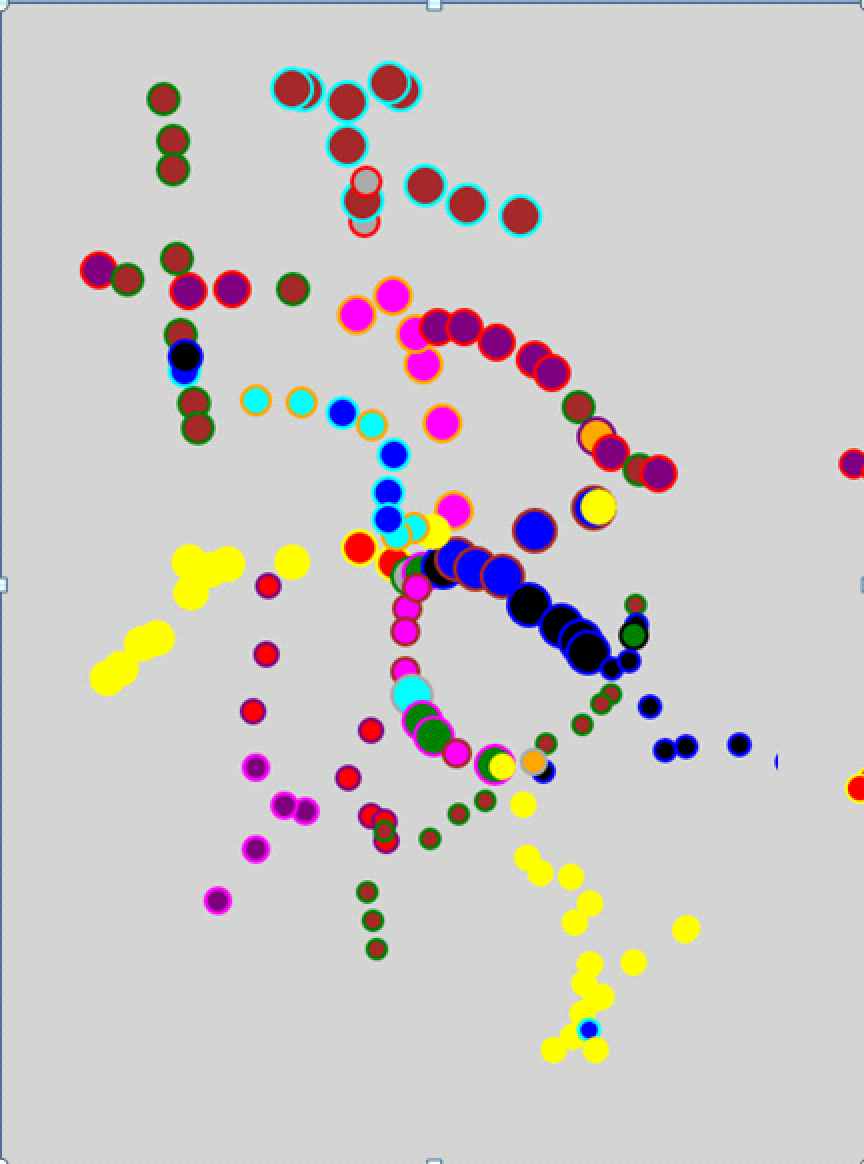
\includegraphics[width=3in]{picture/liuliangbianquan}
						\caption{基于模块化函数的社群划分方法}
						\label{gulidian}
					\end{minipage}
			\end{figure}

		图\ref{gulidian}给出了基本的基于模块化函数的分群结果,首先需要指出:使用基础方法的分群结果收敛于一个具有一千多个解的解集合。最终分群结果会在这些解集合内循环。由图我们可以看出两个问题:

		1)存在很多未被分群的孤立点。

		2)很多社群存在物理意义上的交叉收费站。

		孤立点的产生原因有两个,一是这个收费站本身流量较小,与其他站点交流不多;二是这个站点与其他站点之间的交流较为平均,站点不断流动于不同的社团中。图\ref{fenqun2}是基于公式\ref{eq5}的社群划分结果,该图由几百个社群划分解组成的解集中选出,由图可以看出加入物理路经长度的情况下,可以在一定程度上消除孤立点,并且将高速公路划分成较为清晰的几类。但是我们发现仍旧有少量社群,存在物理层面的相互交叉情况,而这种情况不符合高速公路这种物理网络的社群划分特点。

				\begin{figure}
				\begin{minipage}{0.5\linewidth}
					\centering
					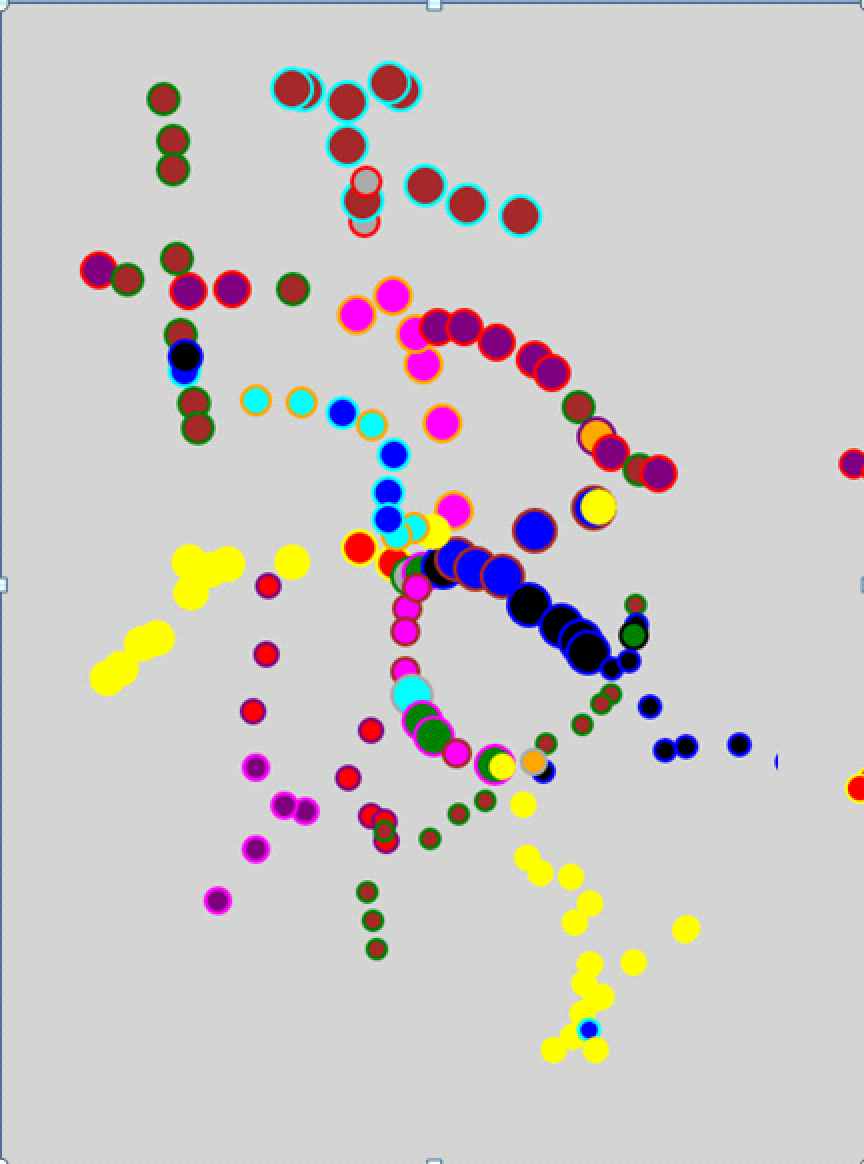
\includegraphics[width=2.2in]{picture/liuliangbianquan}
					\caption{基于模块化函数的社群划分方法}
					\label{fenqun1}
				\end{minipage}%
				\begin{minipage}{0.5\linewidth}
					\centering
					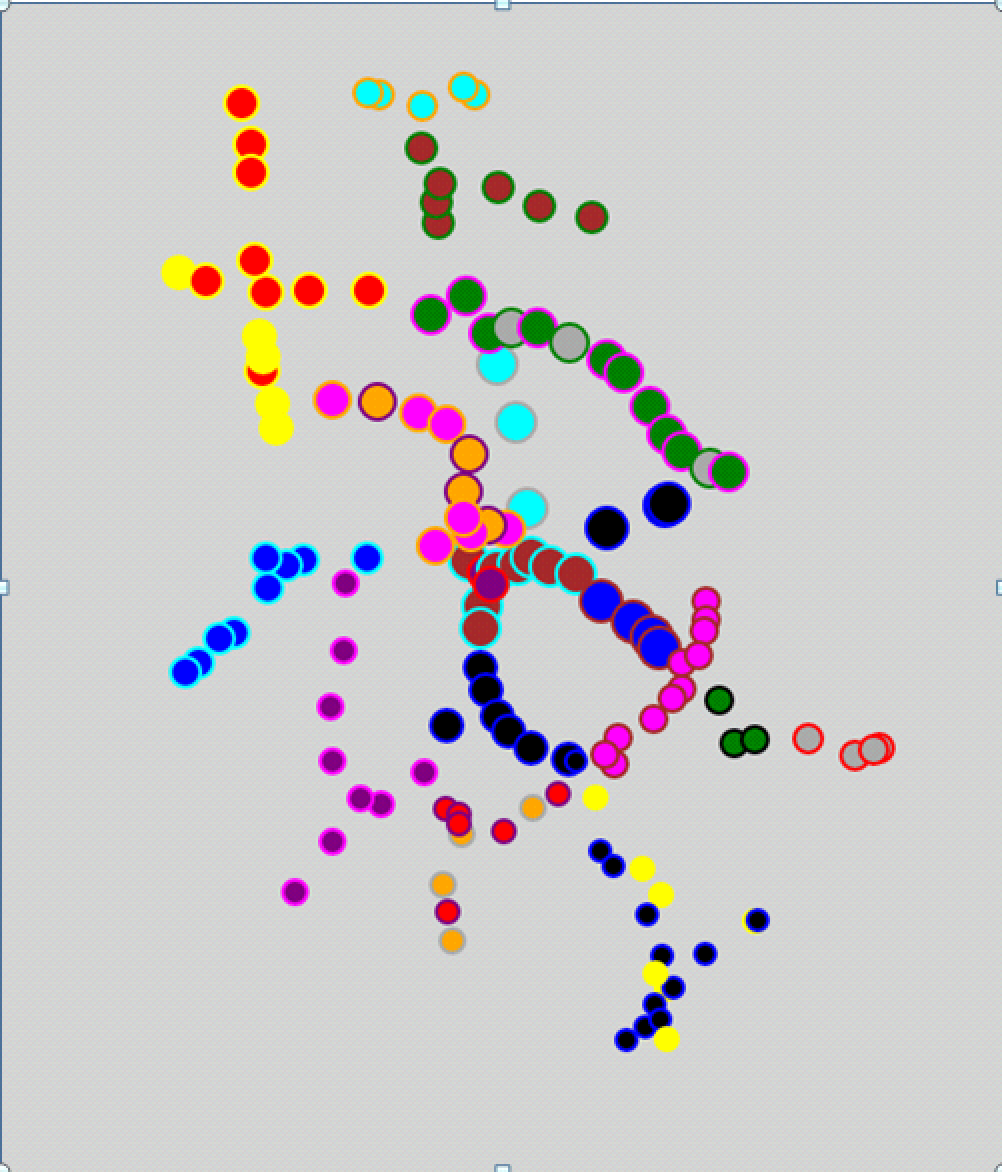
\includegraphics[width=2.5in]{picture/xiaochuguli}
					\caption{结合物理路网特性的社群挖掘}
					\label{fenqun2}
				\end{minipage}
				\end{figure}

		经过数据分析,出现图\ref{fenqun2}中不同社群内部的节点之间存在物理上的交叉情况的原因是——不同社群节点之间的流量差远大于节点之间的距离差。直接将具有交叉节点的社区进行合并虽然简单有效,但是不具有更大规模的适应性,这种方法得到的社群划分效果得不到保证,而且有可能出现过大的社团,不符合社群划分的目的。图\ref{fenqun3}给出了基于模拟退火方法的迭代分群方法结果,该结果最终收敛于由5个结果组成的结果集,基本消除所有孤立点与社群交叉节点。


				\begin{figure}
				\centering
				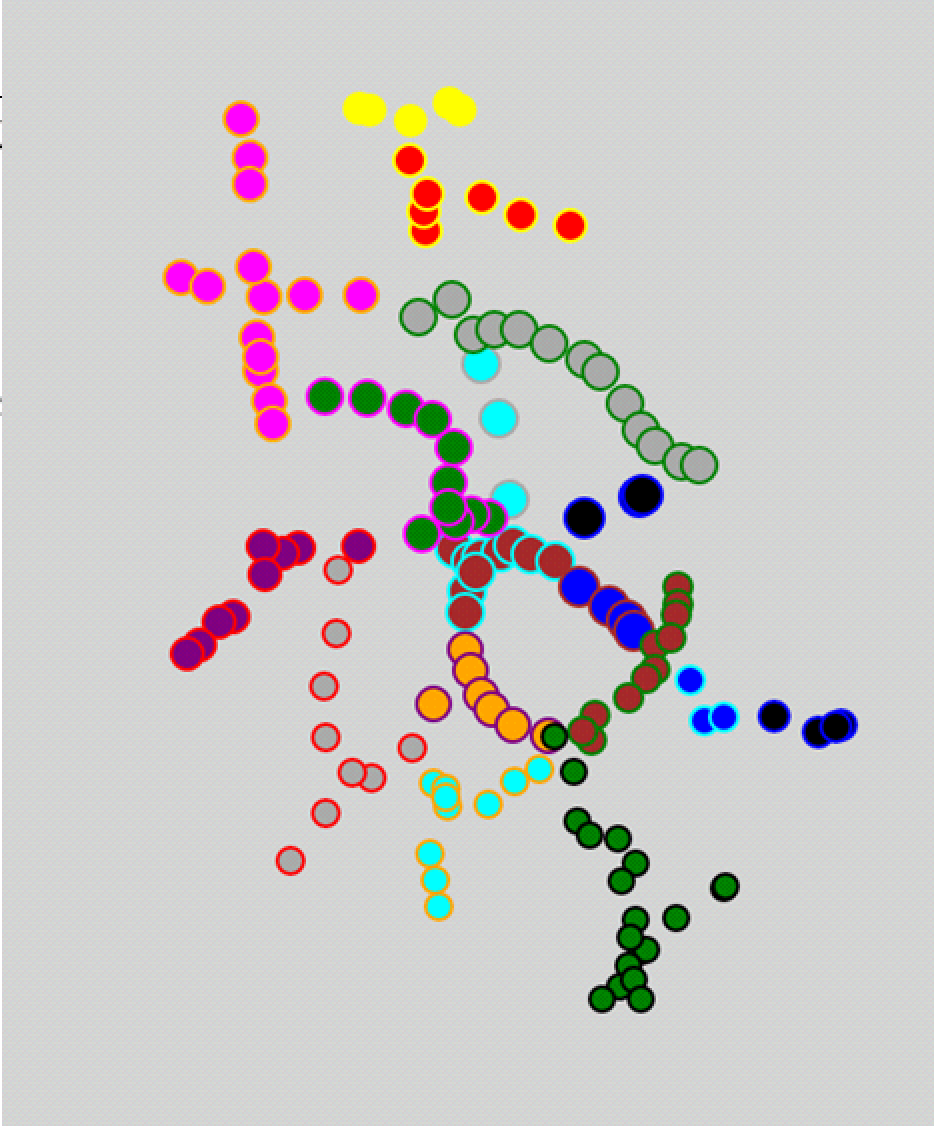
\includegraphics[width=3in]{picture/fenqunjieguo}
				\caption{结合路段距离的变权社群挖掘结果}
				\label{fenqun3}
				\end{figure}

		根据公式\ref{eq4}给出的模块化函数Q,表\ref{table10}给出了不同社群方法模块化的效果。可以看出将边权与物理距离结合考虑后,模块化效果得到了显著提高;虽然模拟退火方法的时间消耗较大,但是它提供了符合物理网络的分群结果,减少不同社群之间的交叉节点,将不同社群之间节点的相互影响降到最低。

				\begin{table}[h]
				\centering
				\begin{tabular}{|c|c|c|c|}
				\hline
				\hline
				   &   基于流量划分 &   基于流量/距离划分 &   基于变化距离的模拟退火  \\
				\hline
				  模块化效果 &   -1321.21 &   -1025.50 &   -1182.84  \\
				\hline
				  算法效率 &   1min &  30s   &   1.5min  \\
				\hline
				  收敛度 &   $10^3$ &   $10^2$ &   $0-10$  \\
				\hline
				\end{tabular}
				\caption{不同社群划分方法效果对比}
				\label{table10}
				\end{table} 



		图\ref{fenqunend}给出了一天时间内,基于分群算法和简单贪心方法的对比试验;图\ref{end}给出了在一周时间内两种方法的对比试验。和上一章节一样,横坐标表示时间,纵坐标表示路网通行效率的绝对值(路网通行时间)。由图可以看出,简单贪心算法和基于分群算法的关键路段挖掘算法之间的误差较为平稳,并且一直维持在一个较低的水平线上。由图可以看出,分群算法可以在和统计算法相似的时间复杂度上,得到比统计算法优秀的解集。

				\begin{figure}
				\begin{minipage}{0.5\linewidth}
					\centering
					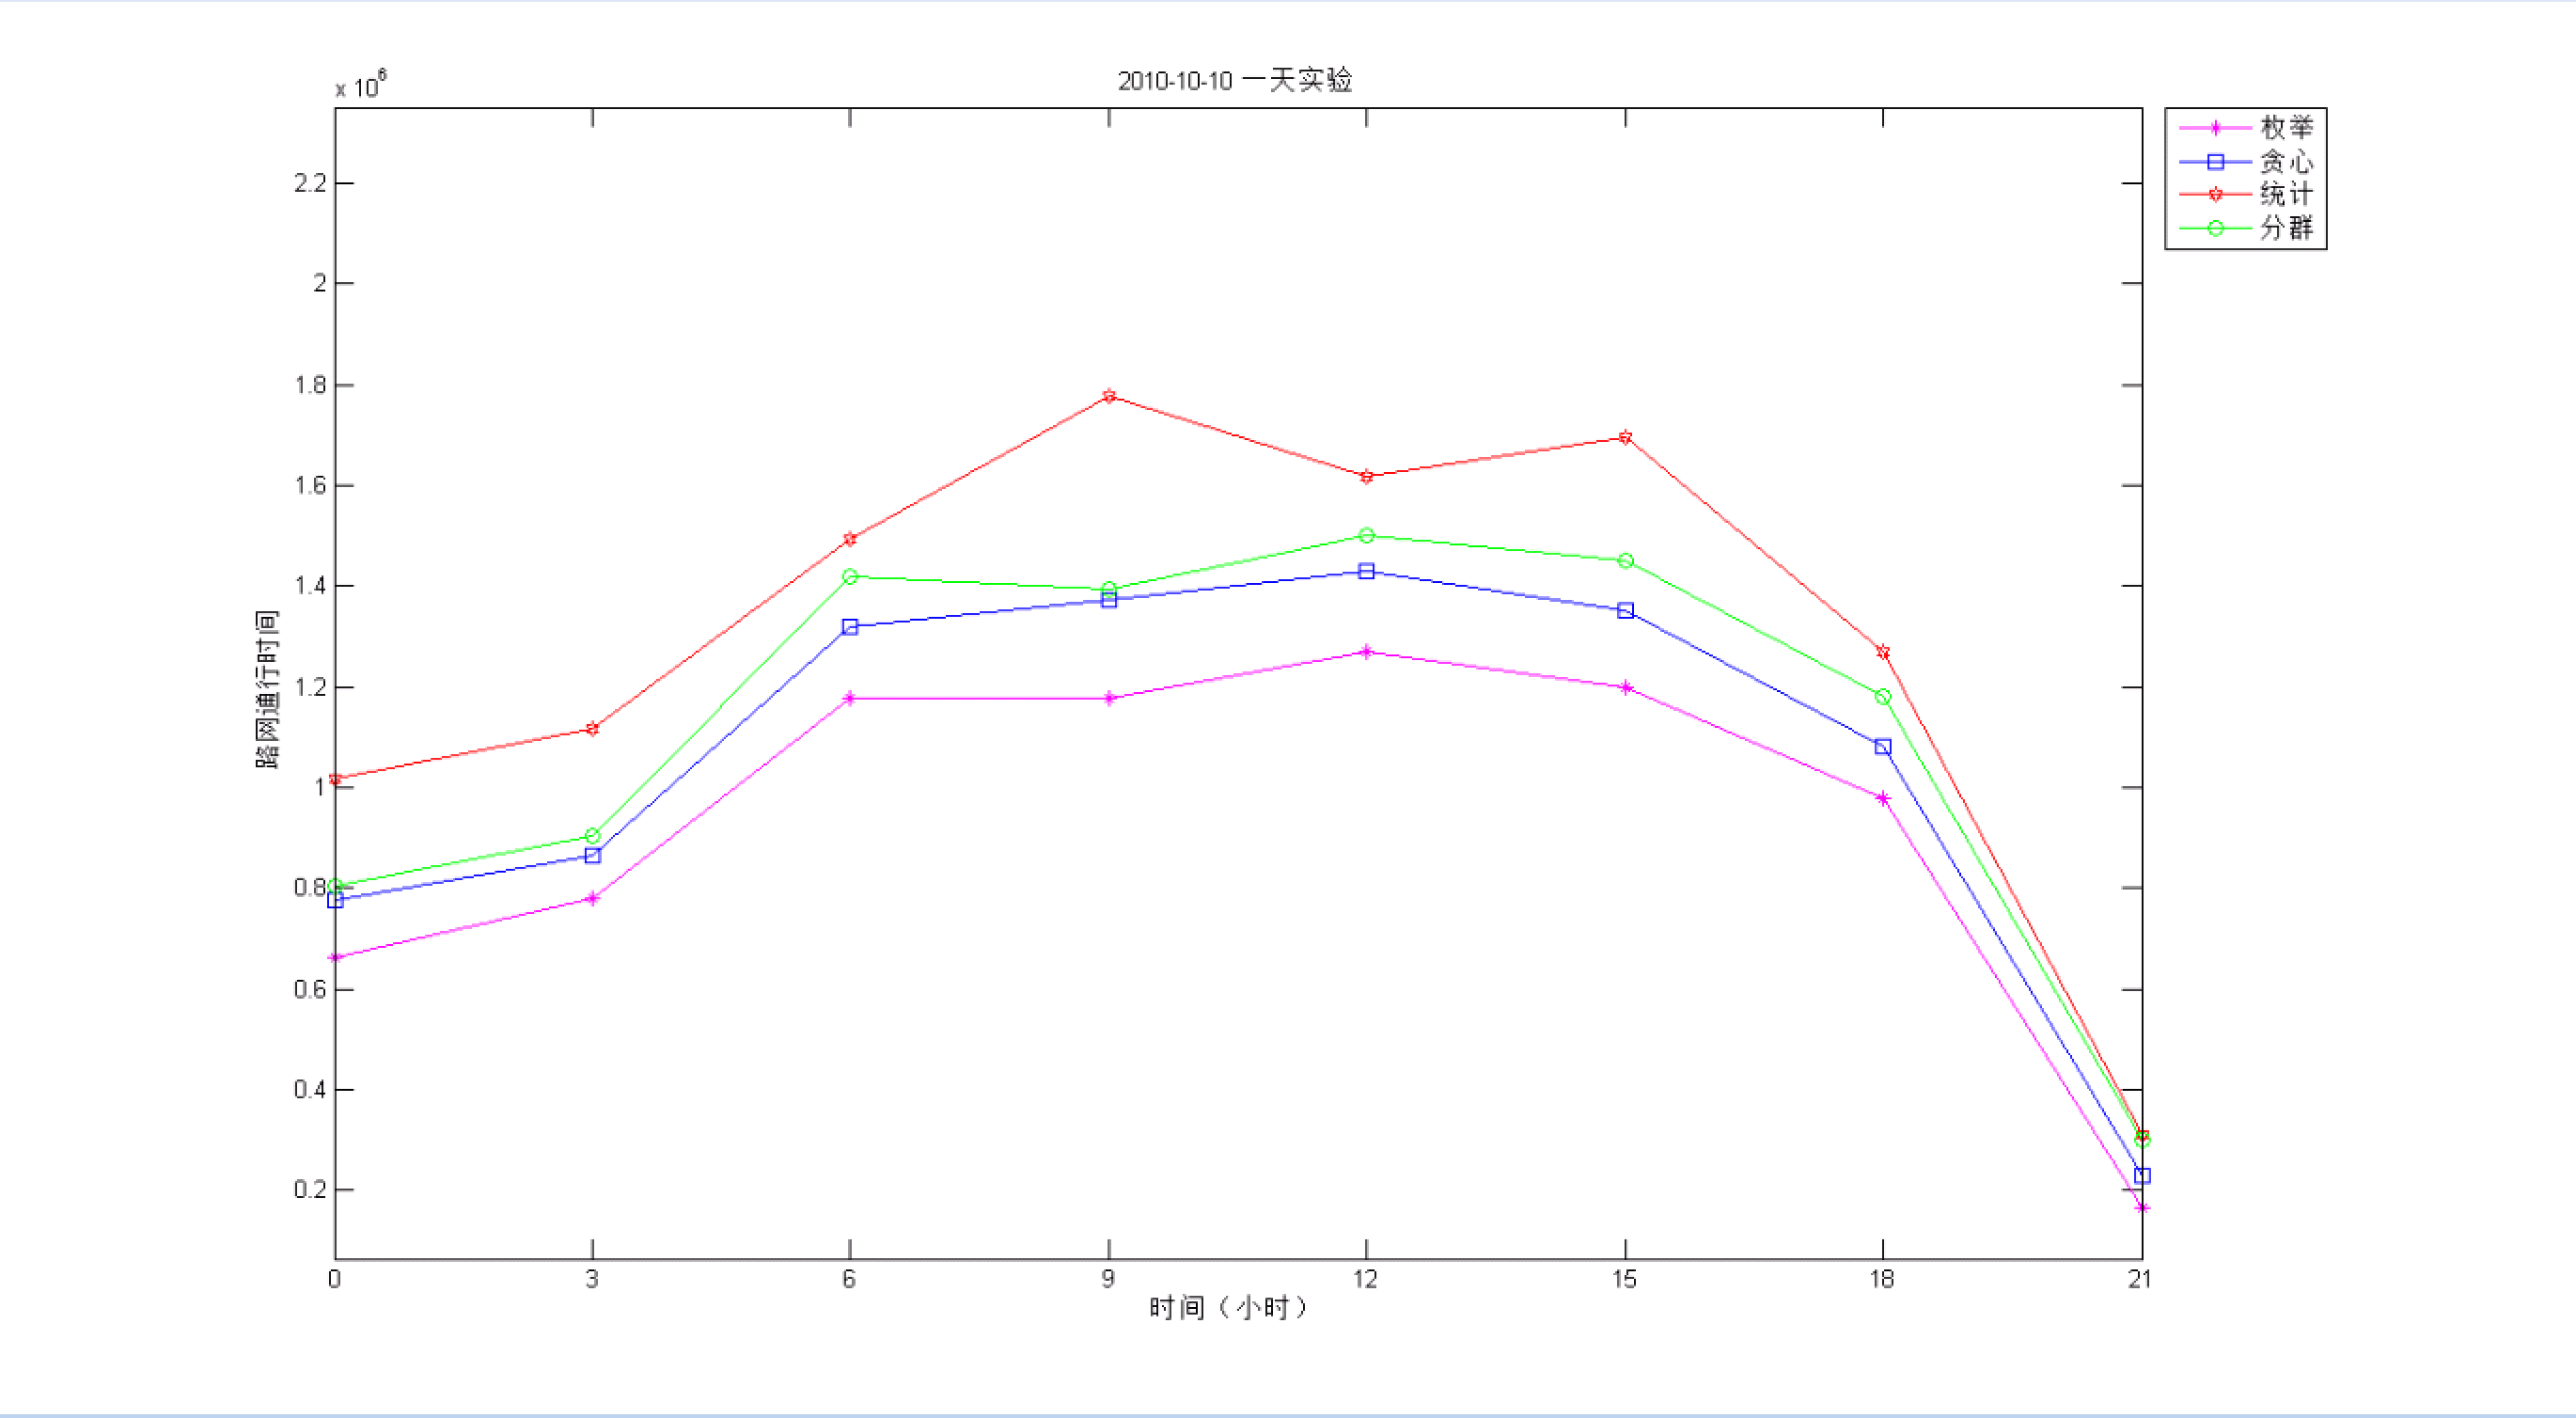
\includegraphics[width=3in]{picture/fenqunend}
					\caption{对比实验:以1h为区间}
					\label{fenqunend}
				\end{minipage}%
				\begin{minipage}{0.5\linewidth}
					\centering
					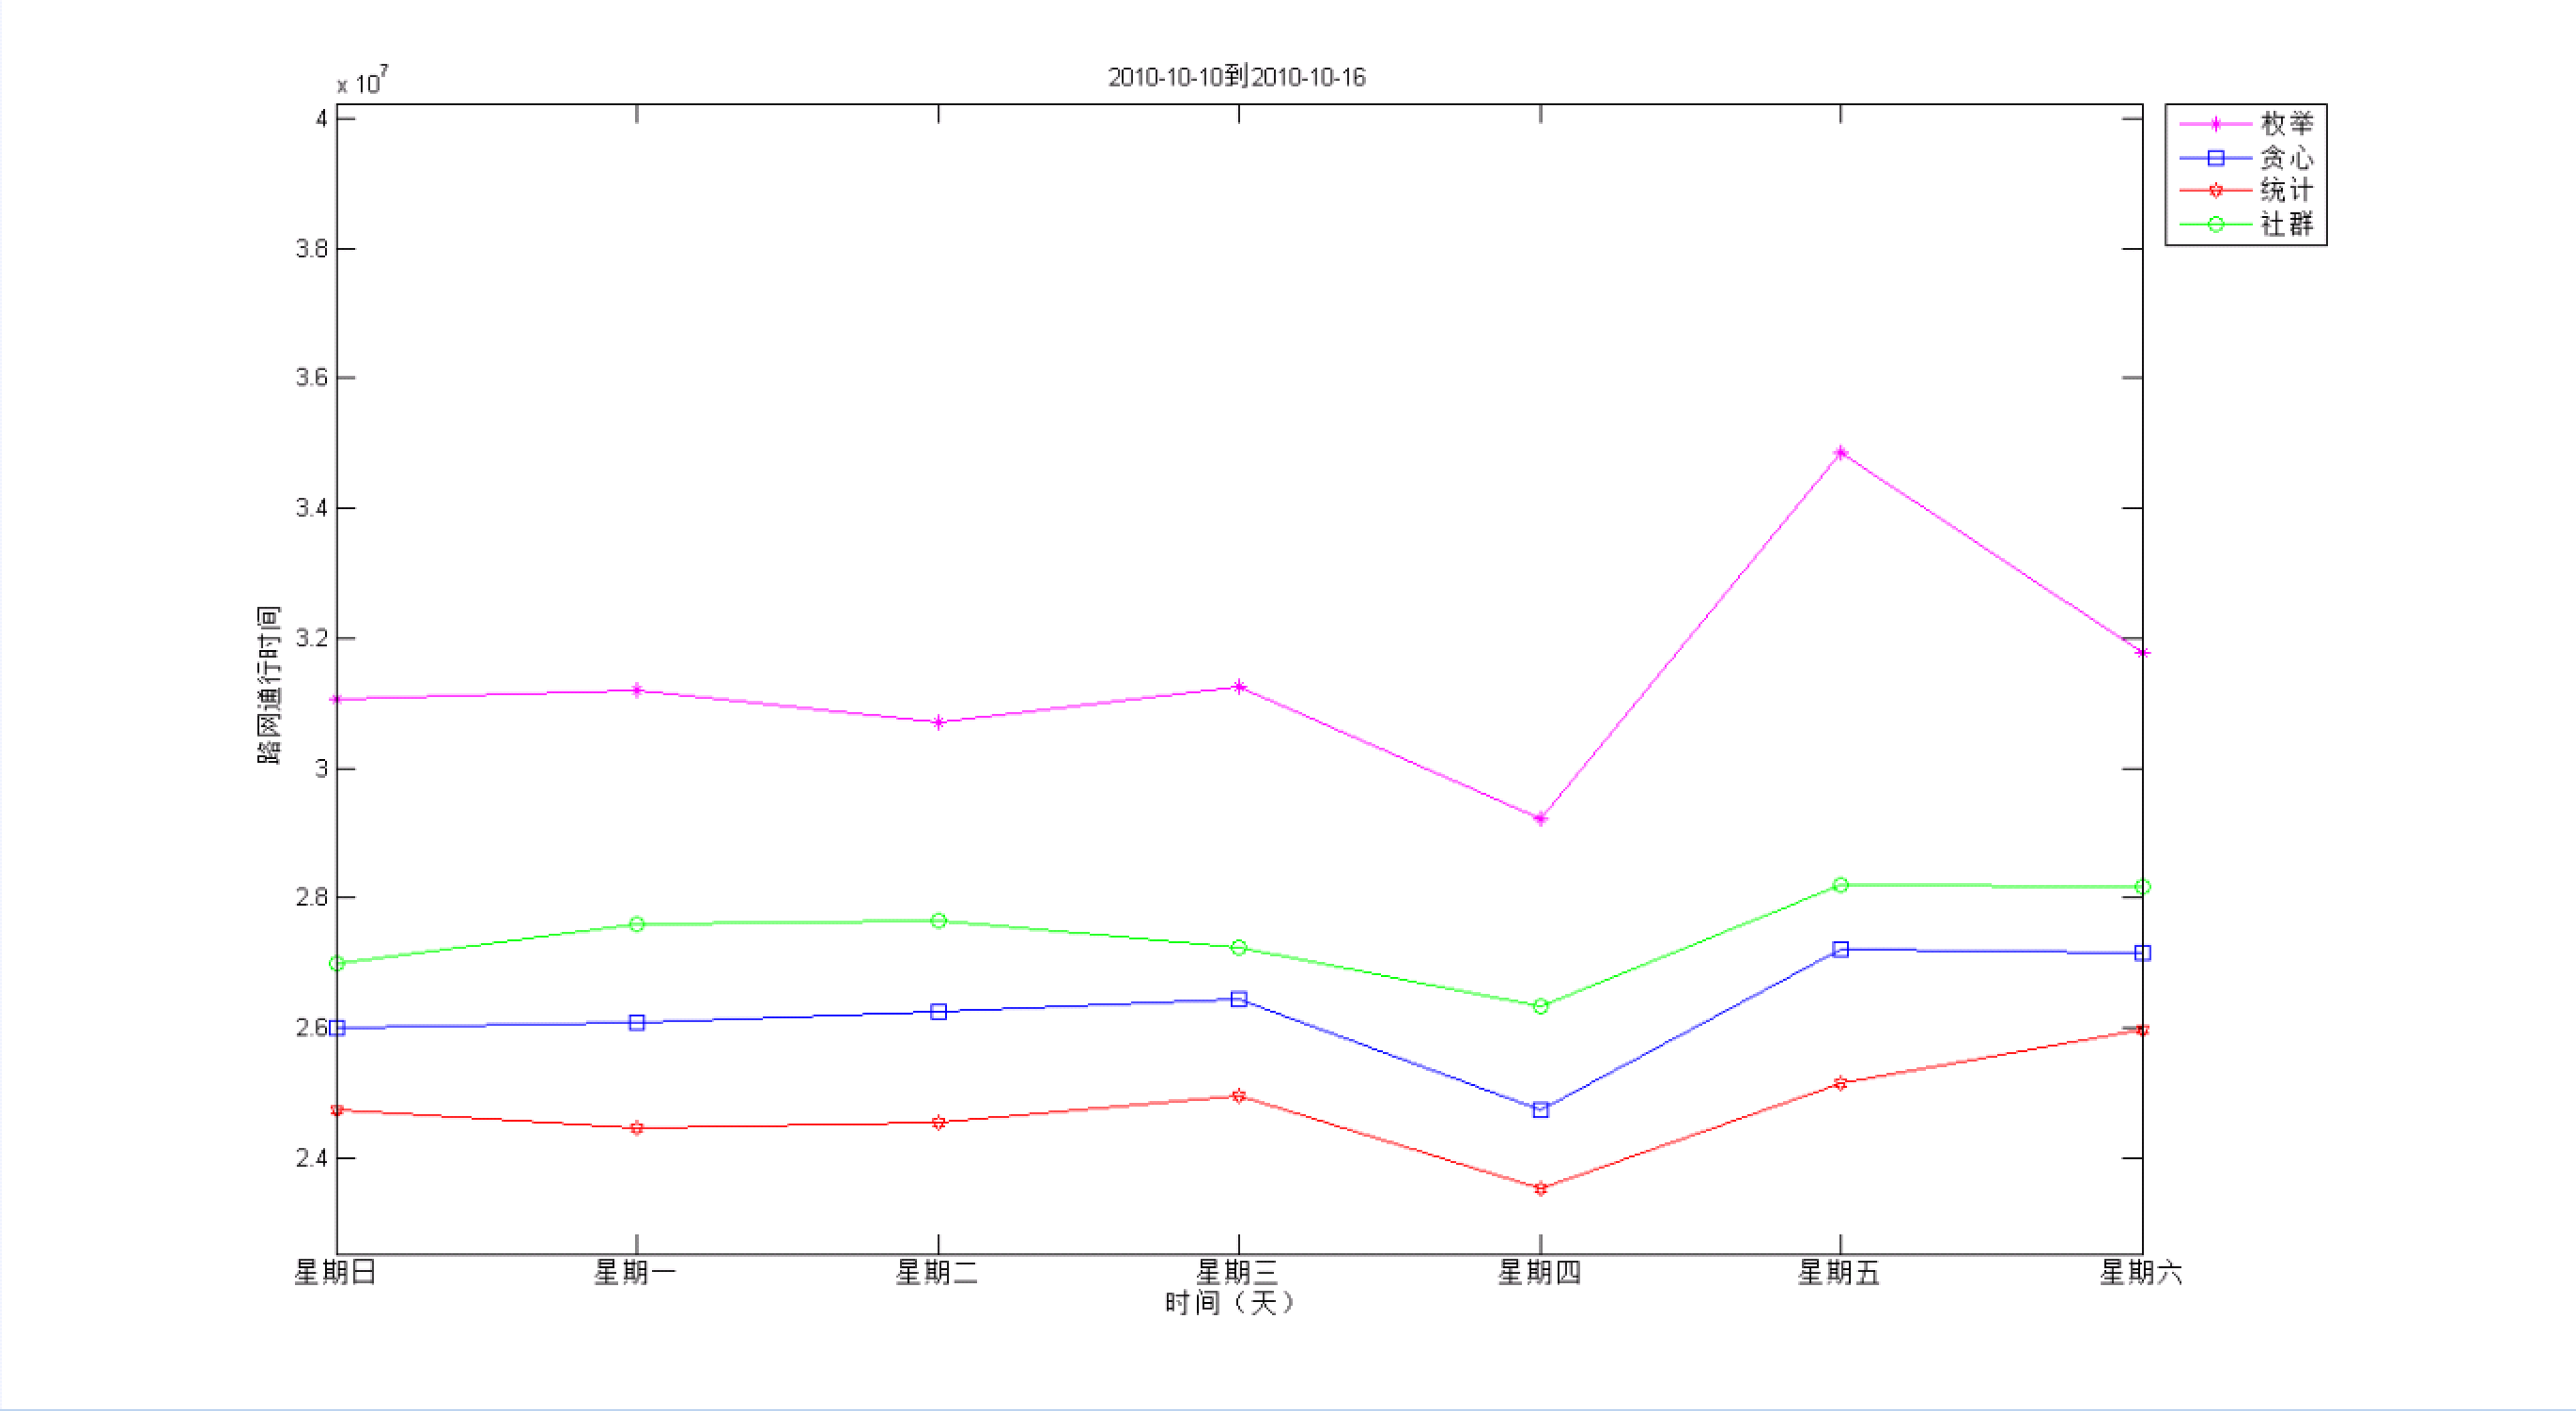
\includegraphics[width=3in]{picture/end}
					\caption{对比实验:以1d为区间}
					\label{end}
				\end{minipage}
				\end{figure}

		下图给出不同方法选出的关键路段集合,图\ref{jihe1}给出了枚举方法选出的关键路段集合,图\ref{jihe2}给出了简单贪心算法给出的关键路段集合,图\ref{jihe3}给出了结合社群划分的关键路段识别算法的结果,图\ref{jihe4}给出了基于统计学的关键路段集合。观察图\ref{jihe1}和图\ref{jihe2},发现两者选取的关键路段具有很强的相似性。

				\begin{figure}
				\begin{minipage}{0.5\linewidth}
					\centering
					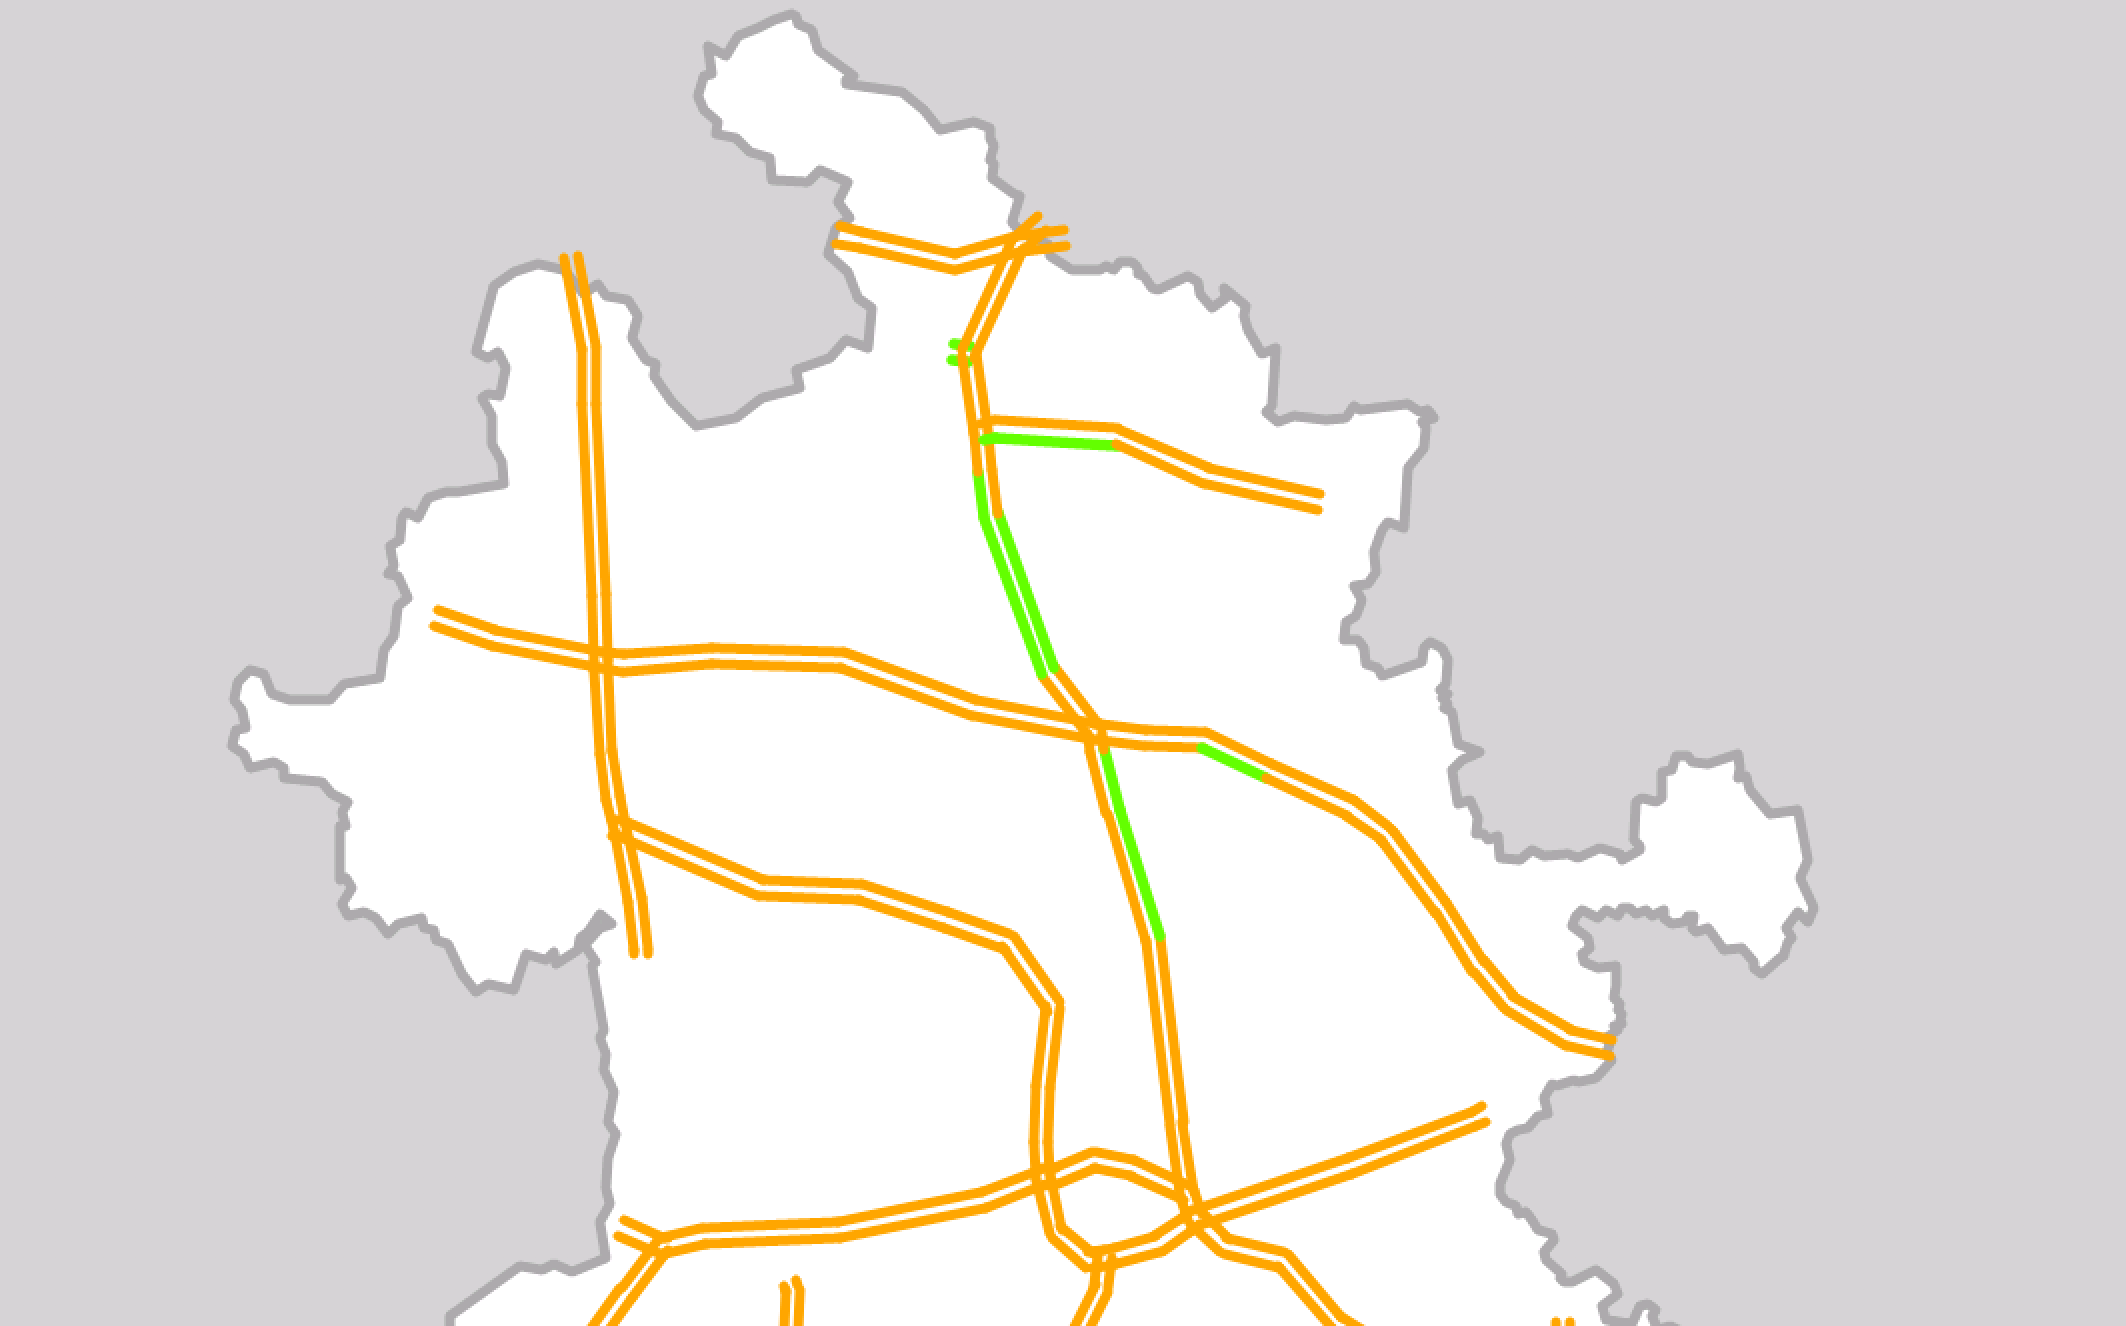
\includegraphics[width=3in]{picture/meiju}
					\caption{枚举求得关键路段}
					\label{jihe1}
				\end{minipage}%
				\begin{minipage}{0.5\linewidth}
					\centering
					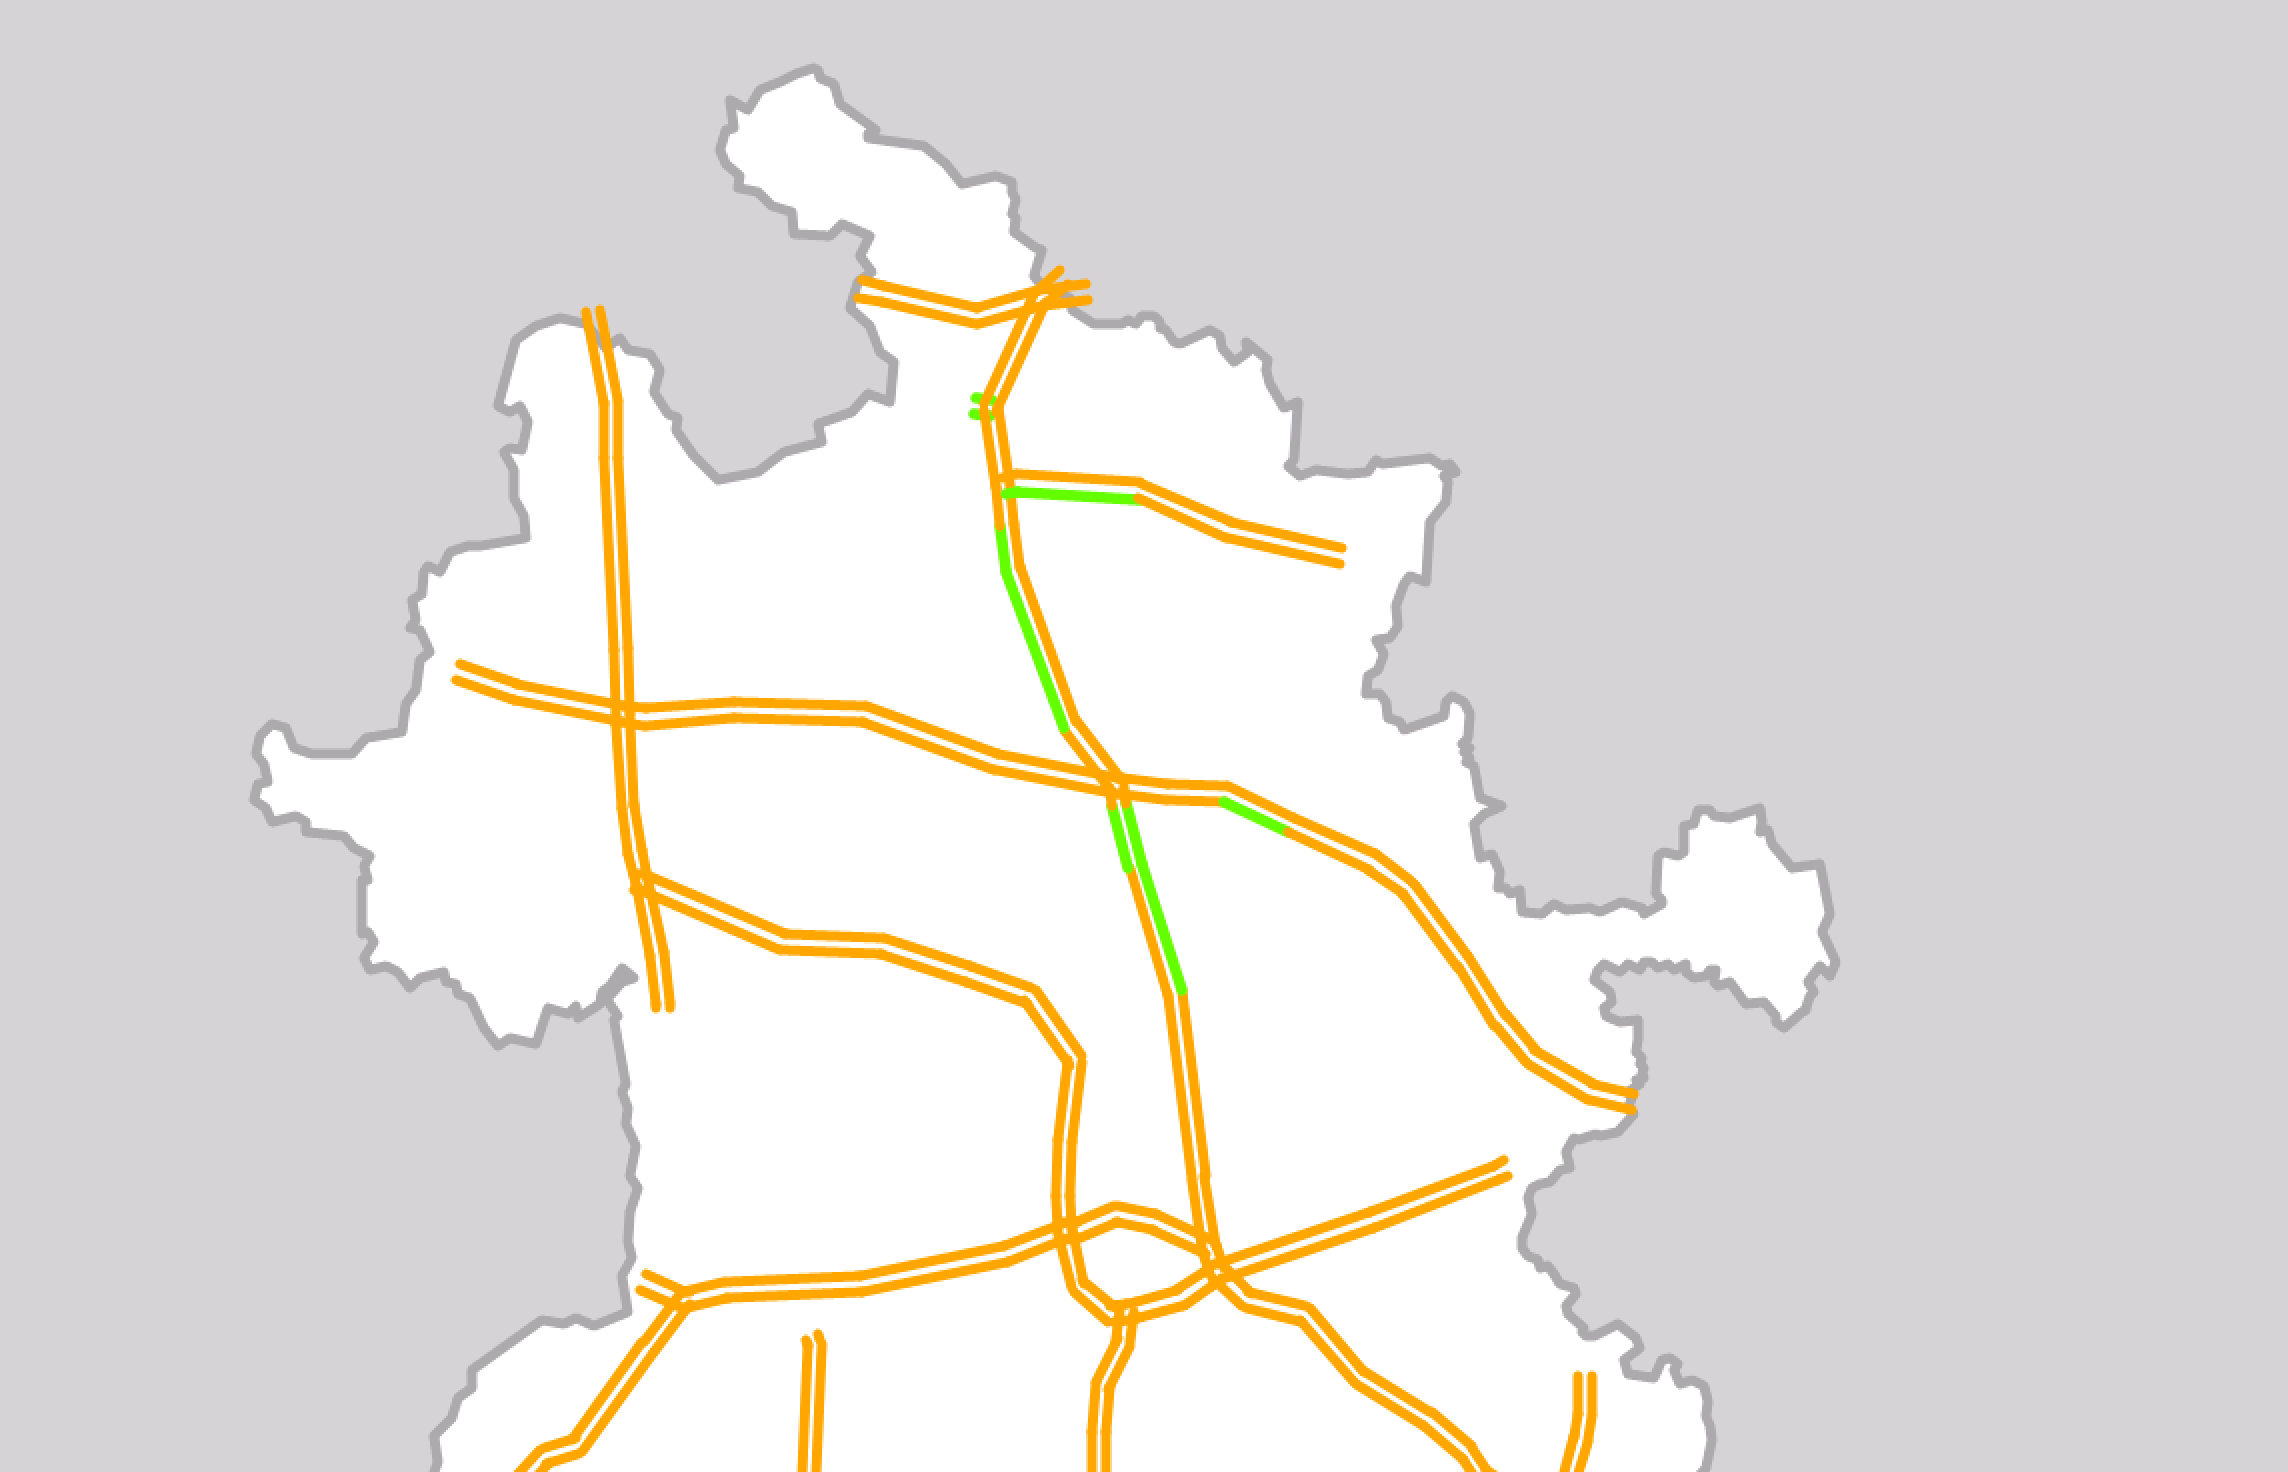
\includegraphics[width=3in]{picture/tanxin}
					\caption{贪心求得关键路段}
					\label{jihe2}
				\end{minipage}
				\end{figure}

				\begin{figure}
				\begin{minipage}{0.5\linewidth}
					\centering
					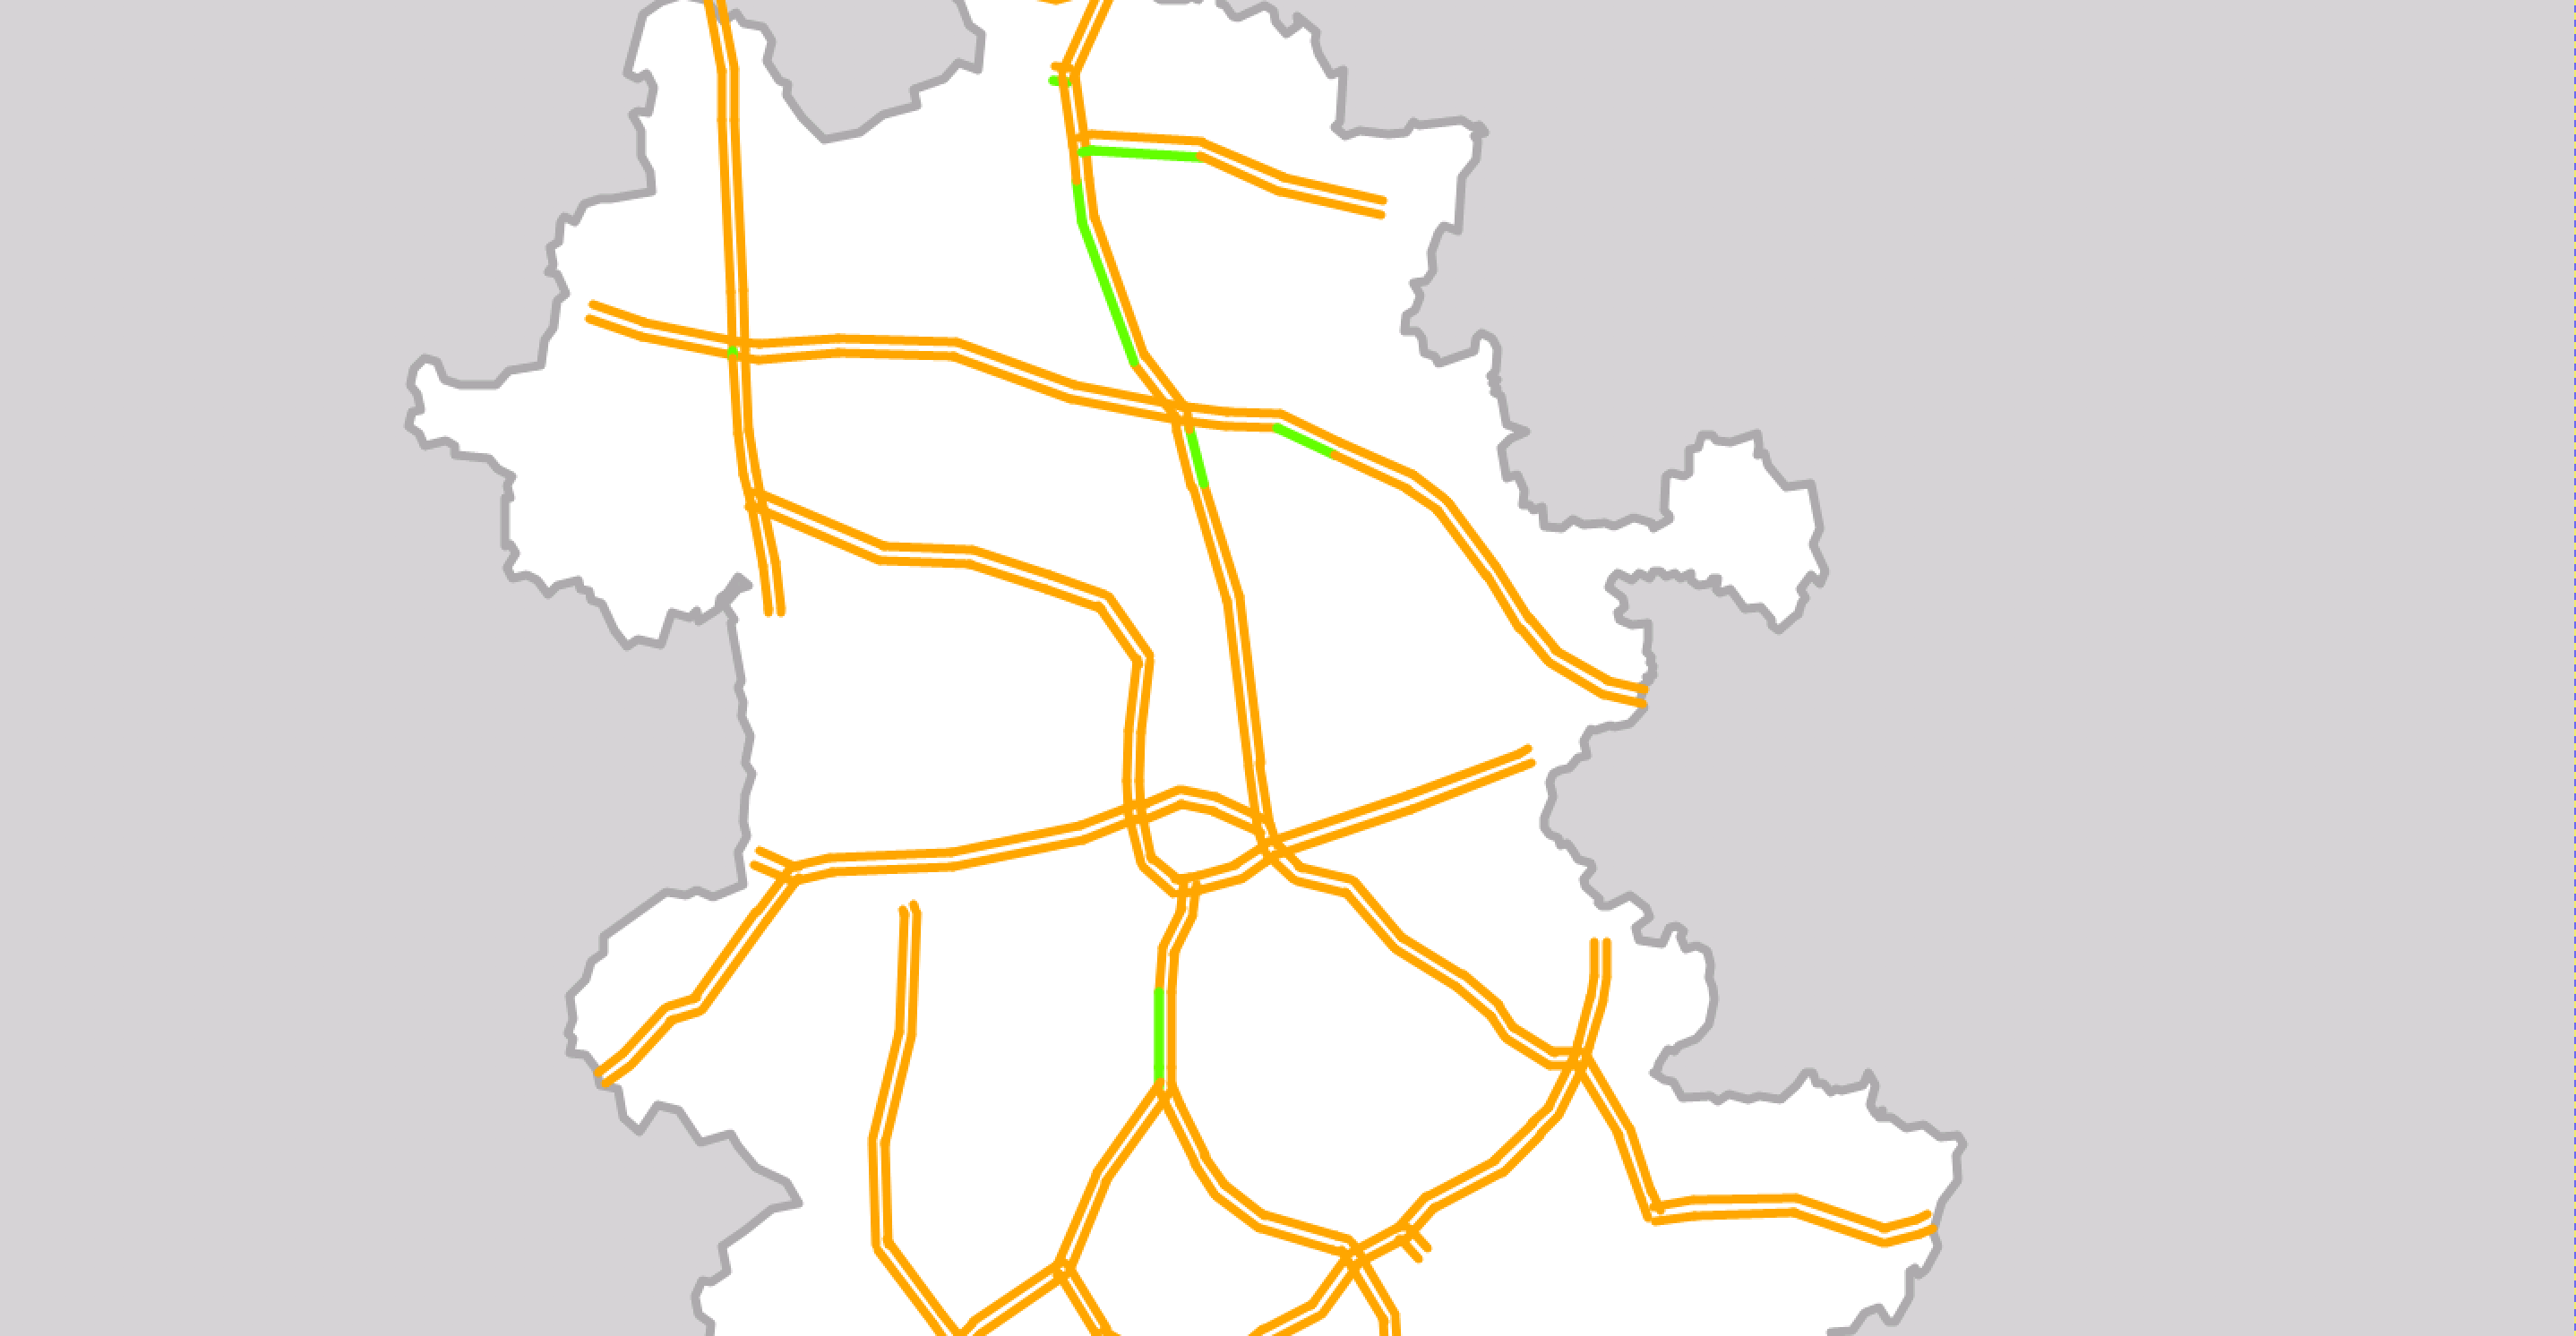
\includegraphics[width=3in]{picture/fenqun}
					\caption{基于社群划分的关键路段}
					\label{jihe3}
				\end{minipage}%
				\begin{minipage}{0.5\linewidth}
					\centering
					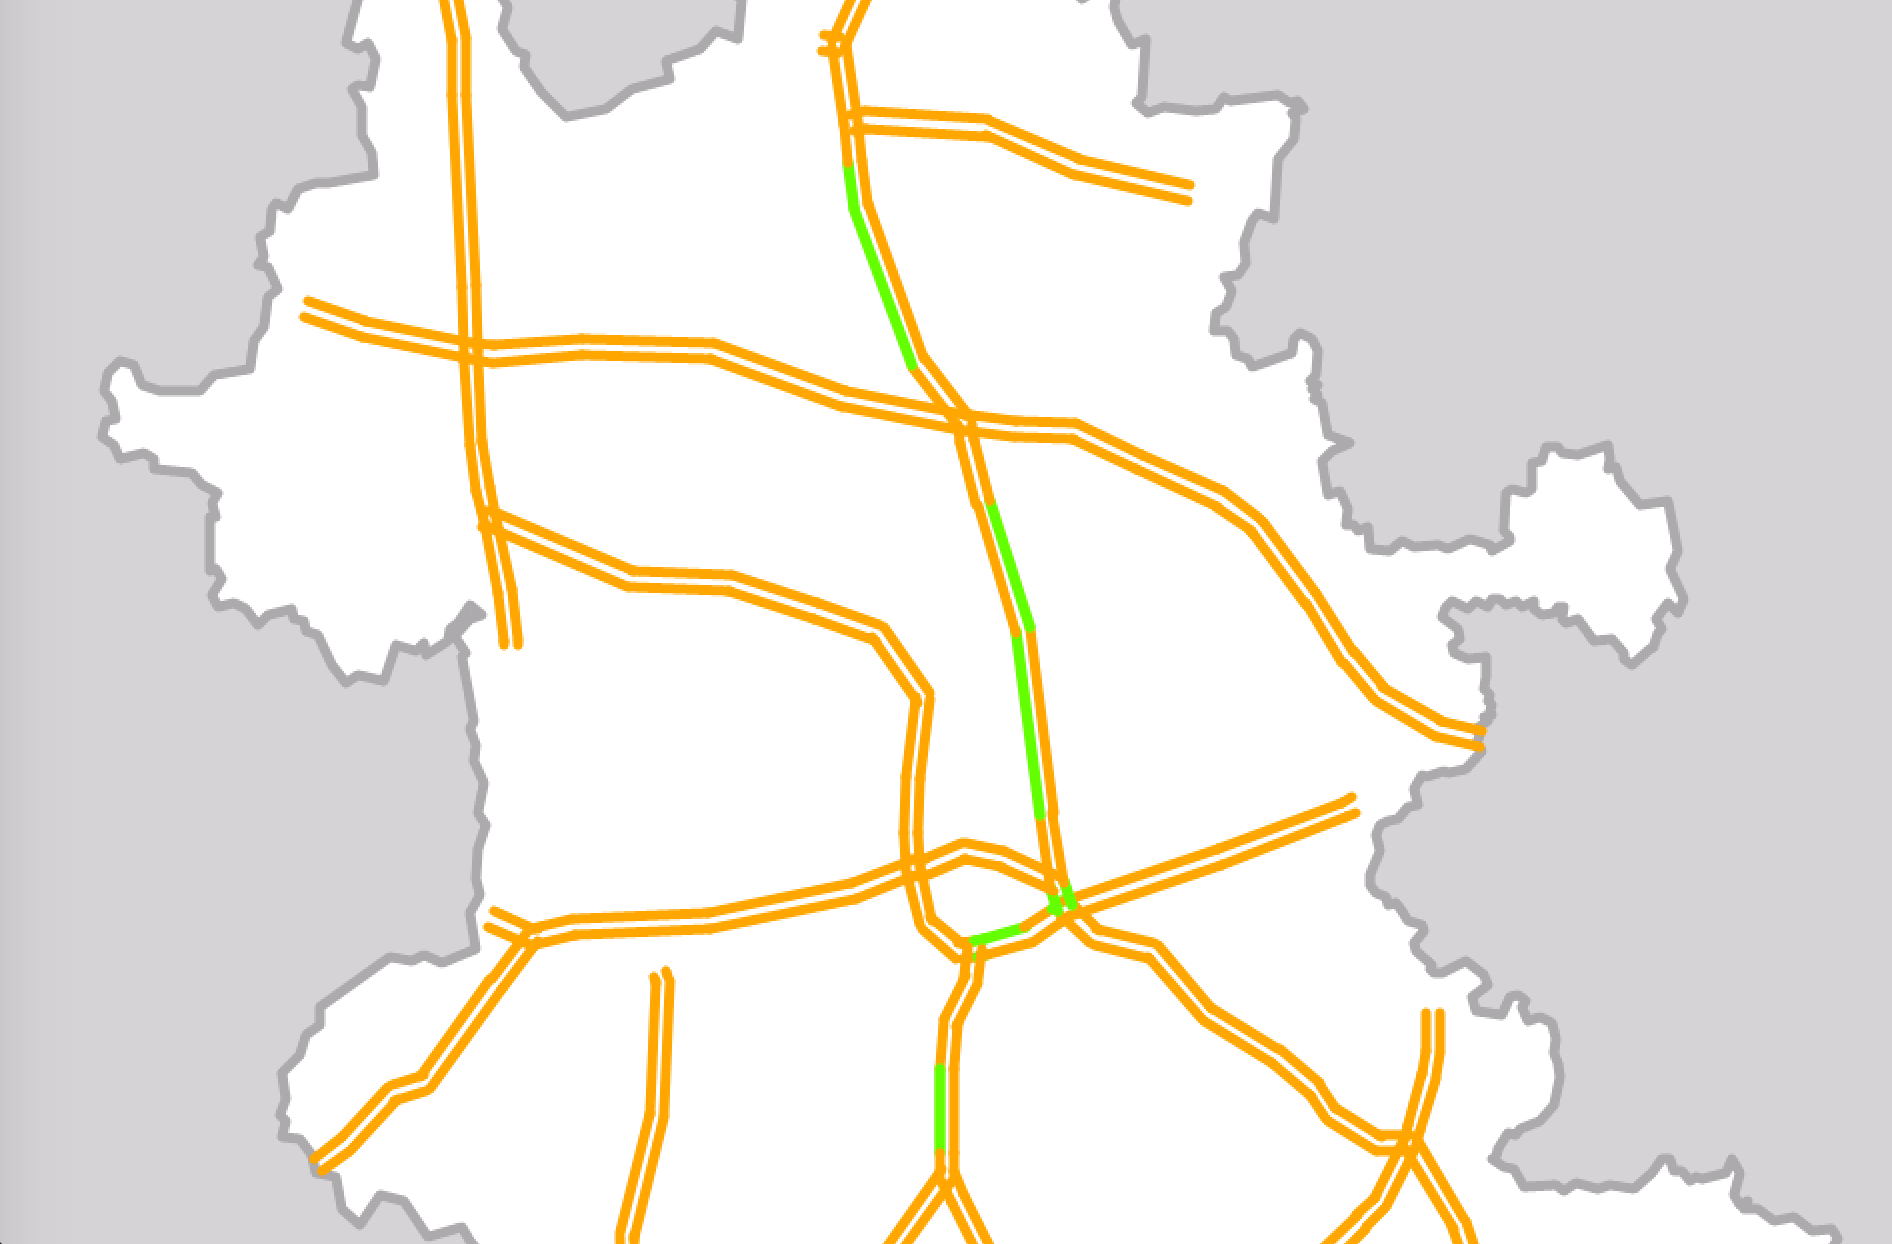
\includegraphics[width=2.5in]{picture/hotsection}
					\caption{基于统计学的关键路段}
					\label{jihe4}
				\end{minipage}
				\end{figure}

		误差分析:

				\begin{table}[h]
				\centering
				\begin{tabular}{|c|c|c|}
				\hline
				\hline
				  &  枚举-直接贪心 &  直接贪心-基于社群划分 \\
				\hline
				 一小时 &  14.63\% &  12.89\% \\
				\hline
				 一天 &  13.25\% &  13.26\% \\
				\hline
				 一周 &  13.10\% &  15.61\% \\
				\hline
				 一月 &  12.99\% &  11.59\% \\
				\hline
				\end{tabular}
				\caption{路网通行效率提升量误差分析}
				\label{table1}
				\end{table} 

		表\ref{table1}描述了枚举方法和直接贪心方法之间的误差,直接贪心和基于社群划分方法之间的误差。误差由高速路网的通行效率计算,可以看出误差在允许范围内。

		关键路段选取误差分析:

				\begin{table}[h]
				\centering
				\begin{tabular}{|c|c|c|}
				\hline
				\hline
				   &   枚举-直接贪心 &   枚举-基于社群划分 \\
				\hline
				  一小时 &   0.18\% &   0.25\% \\
				\hline
				  一天 &   0.14\% &   0.20\% \\
				\hline
				  一周 &   0.15\% &   0.19\% \\
				\hline
				  一月 &   0.14\% &   0.18\% \\
				\hline
				\end{tabular}
				\caption{关键路段选取误差分析}
				\label{table2}
				\end{table} 

		表\ref{table2}分析了关键路段选取情况的误差,采用欧式距离来刻画区别。可以看出,随着数据集的扩大,基于社群划分方法的关键路段准确率逐步上升。

		运行效率分析:

				\begin{table}[h]
				\centering
				\begin{tabular}{|c|c|c|c|c|}
				\hline
				\hline
				   &   枚举 &   直接贪心 &   基于社群划分 &   基于统计 \\
				\hline
				  一小时 &   1day &   30min &   2min &   1min \\
				\hline
				  一天 &   6day &   2h &   5min &   2min \\
				\hline
				  一周 &  7day &   3h &   6min &   5min \\
				\hline
				  一月 &   7day &   3h &   7min &   8min \\
				\hline
				\end{tabular}
				\caption{不同方法运行效率分析}
				\label{table3}
				\end{table} 

		由表\ref{table3}可以看出,基于社群划分方法可以将整个算法的时间复杂度再降一个数量级,而结合表\ref{table1}来看,精度误差处于可接受范围$(1/e)$。

	\section{本章小结}
		本章提出了面向高速公路的社群划分方法,首先分析了传统方法的局限性,然后结合高速公路的独有特性,采用多变权值-模拟退火结合的方法,实现符合高速公路网络特点的社群划分方法。最后结合动态规划方法,实现多项式时间求解。
	% vim:ts=4:sw=4
% Copyright (c) 2014 Casper Ti. Vector
% Public domain.

\chapter{原型系统的设计与实现}
	\section{系统架构}
		高速公路关键路段识别算法是为了解决高速公路管理者解决高速公路资源配比问题而开发的,整个系统基于B/S架构,从高层划分为前端和后端两部分,具体系统架构见图\ref{fig20},后端为Windows服务,主要包括实时车辆数据的处理以及数据仓库的存储。前端系统中,我们编写自己的业务逻辑,Web Service和展现系统,通过调用已有的数据访问层进行数据处理,完成系统任务。

		\begin{figure}[h]
		\centering
				\begin{minipage}{0.8\linewidth}
					\centering
					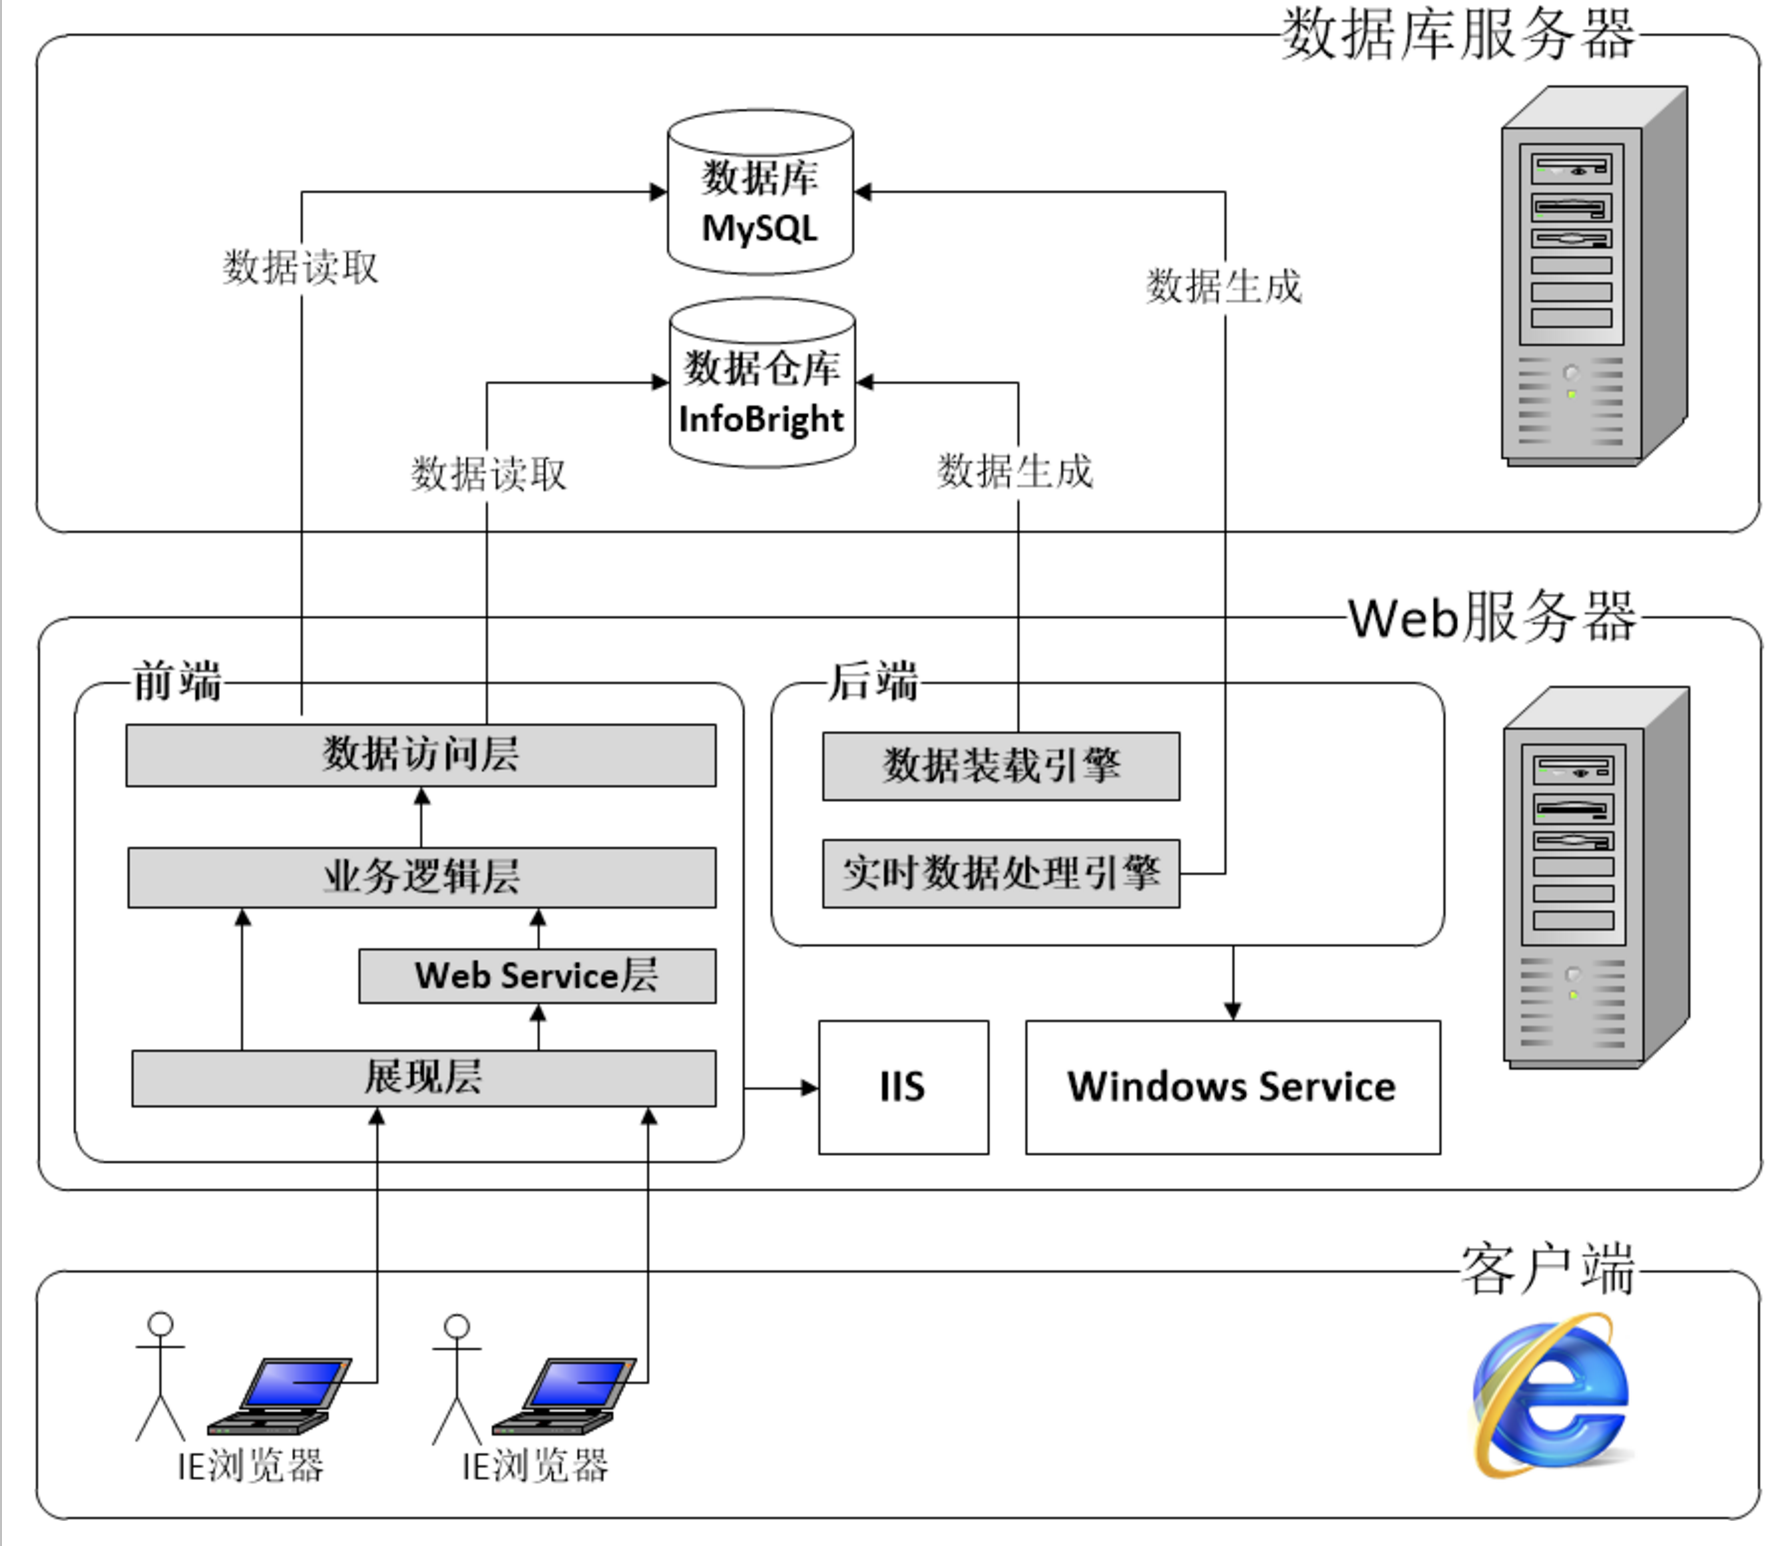
\includegraphics[width=4.4in]{picture/jiagou}
					\caption{智能高速系统架构}
					\label{fig20}
				\end{minipage}%\
		\end{figure}
	\section{结合高速公路分群算法的并行策略}
		系统中,采用hadoop中的map reduce思想,进行效率优化。首先在主机器中进行分群,然后将每一个社群数据map到子机器中,在子机器中计算社群内部的关键节点,之后将结果reduce到主机器中,计算出最终结果。

		流程图见图\ref{mapreduce}:
		\begin{figure}[h]
		\centering
				\begin{minipage}{0.8\linewidth}
					\centering
					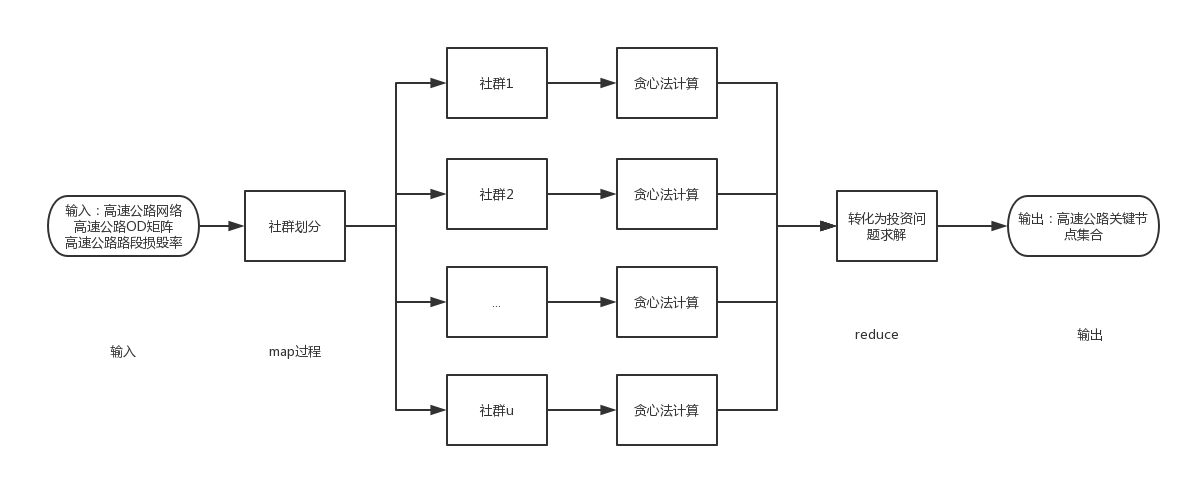
\includegraphics[width=4.4in]{picture/mapreduce}
					\caption{mapreduce流程图}
					\label{mapreduce}
				\end{minipage}%\
		\end{figure}

	\section{系统模块}

		系统主要面向高速公路上重大事故的预防与处理。与城市路网相比,高速公路联网收费数据能够获得准确的用户OD数据,可以有效的进行分析。图\ref{fig21}是关键路段挖掘系统的技术流程图。

		\begin{figure}[h]
		\centering
				\begin{minipage}{0.8\linewidth}
					\centering
					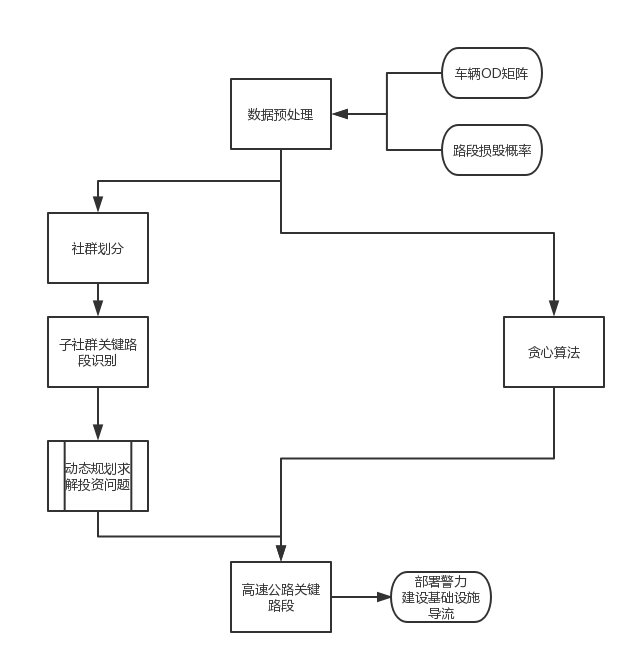
\includegraphics[width=4.4in]{picture/liuchengtu}
					\caption{关键路段挖掘系统流程图}
					\label{fig21}
				\end{minipage}%\
		\end{figure}
		
	\section{界面功能展示}

		系统的输入有时间,时间区间,路段损毁概率,管理者对关键路段的维护效果。

		系统输出两层信息,第一层是关键路段分群效果,如图\ref{yuanxing1};第二层是关键路段选取结果,如图\ref{yuanxing2}。

		\begin{figure}[h]
		\centering
				\begin{minipage}{0.8\linewidth}
					\centering
					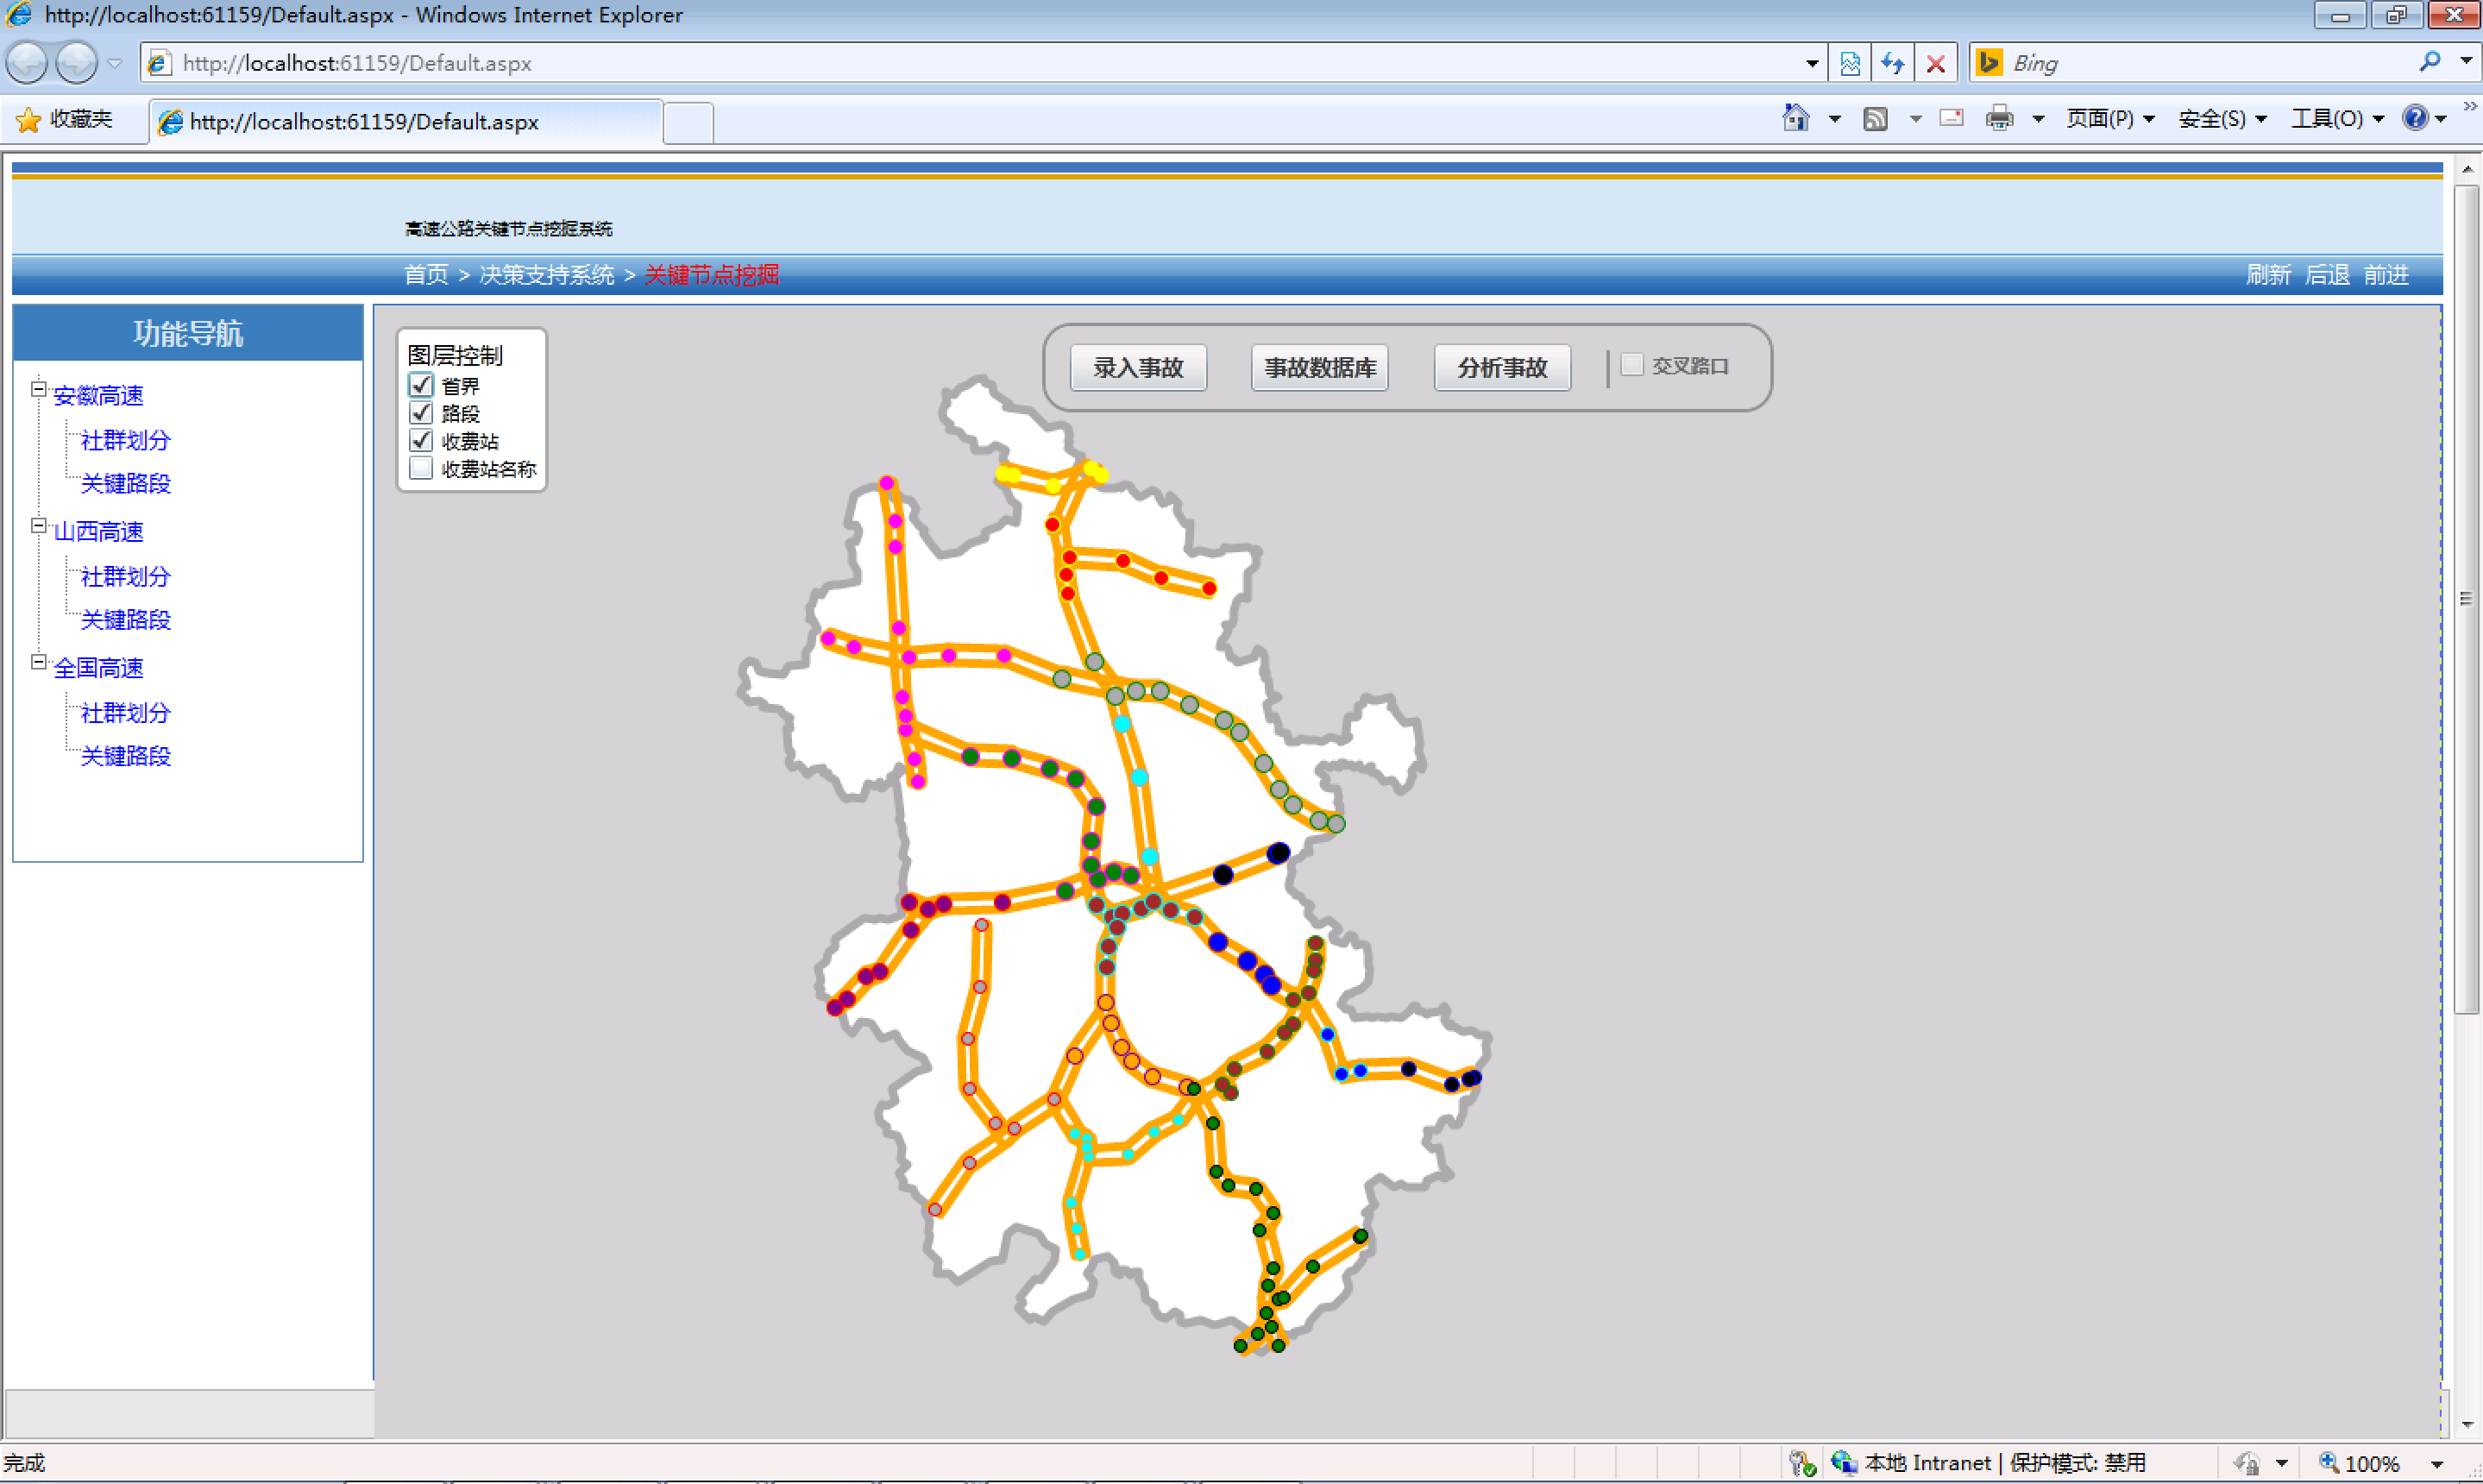
\includegraphics[width=4.4in]{picture/yuanxing1}
					\caption{系统分群结果图}
					\label{fig21}
				\end{minipage}%\
		\end{figure}


		\begin{figure}[h]
		\centering
				\begin{minipage}{0.8\linewidth}
					\centering
					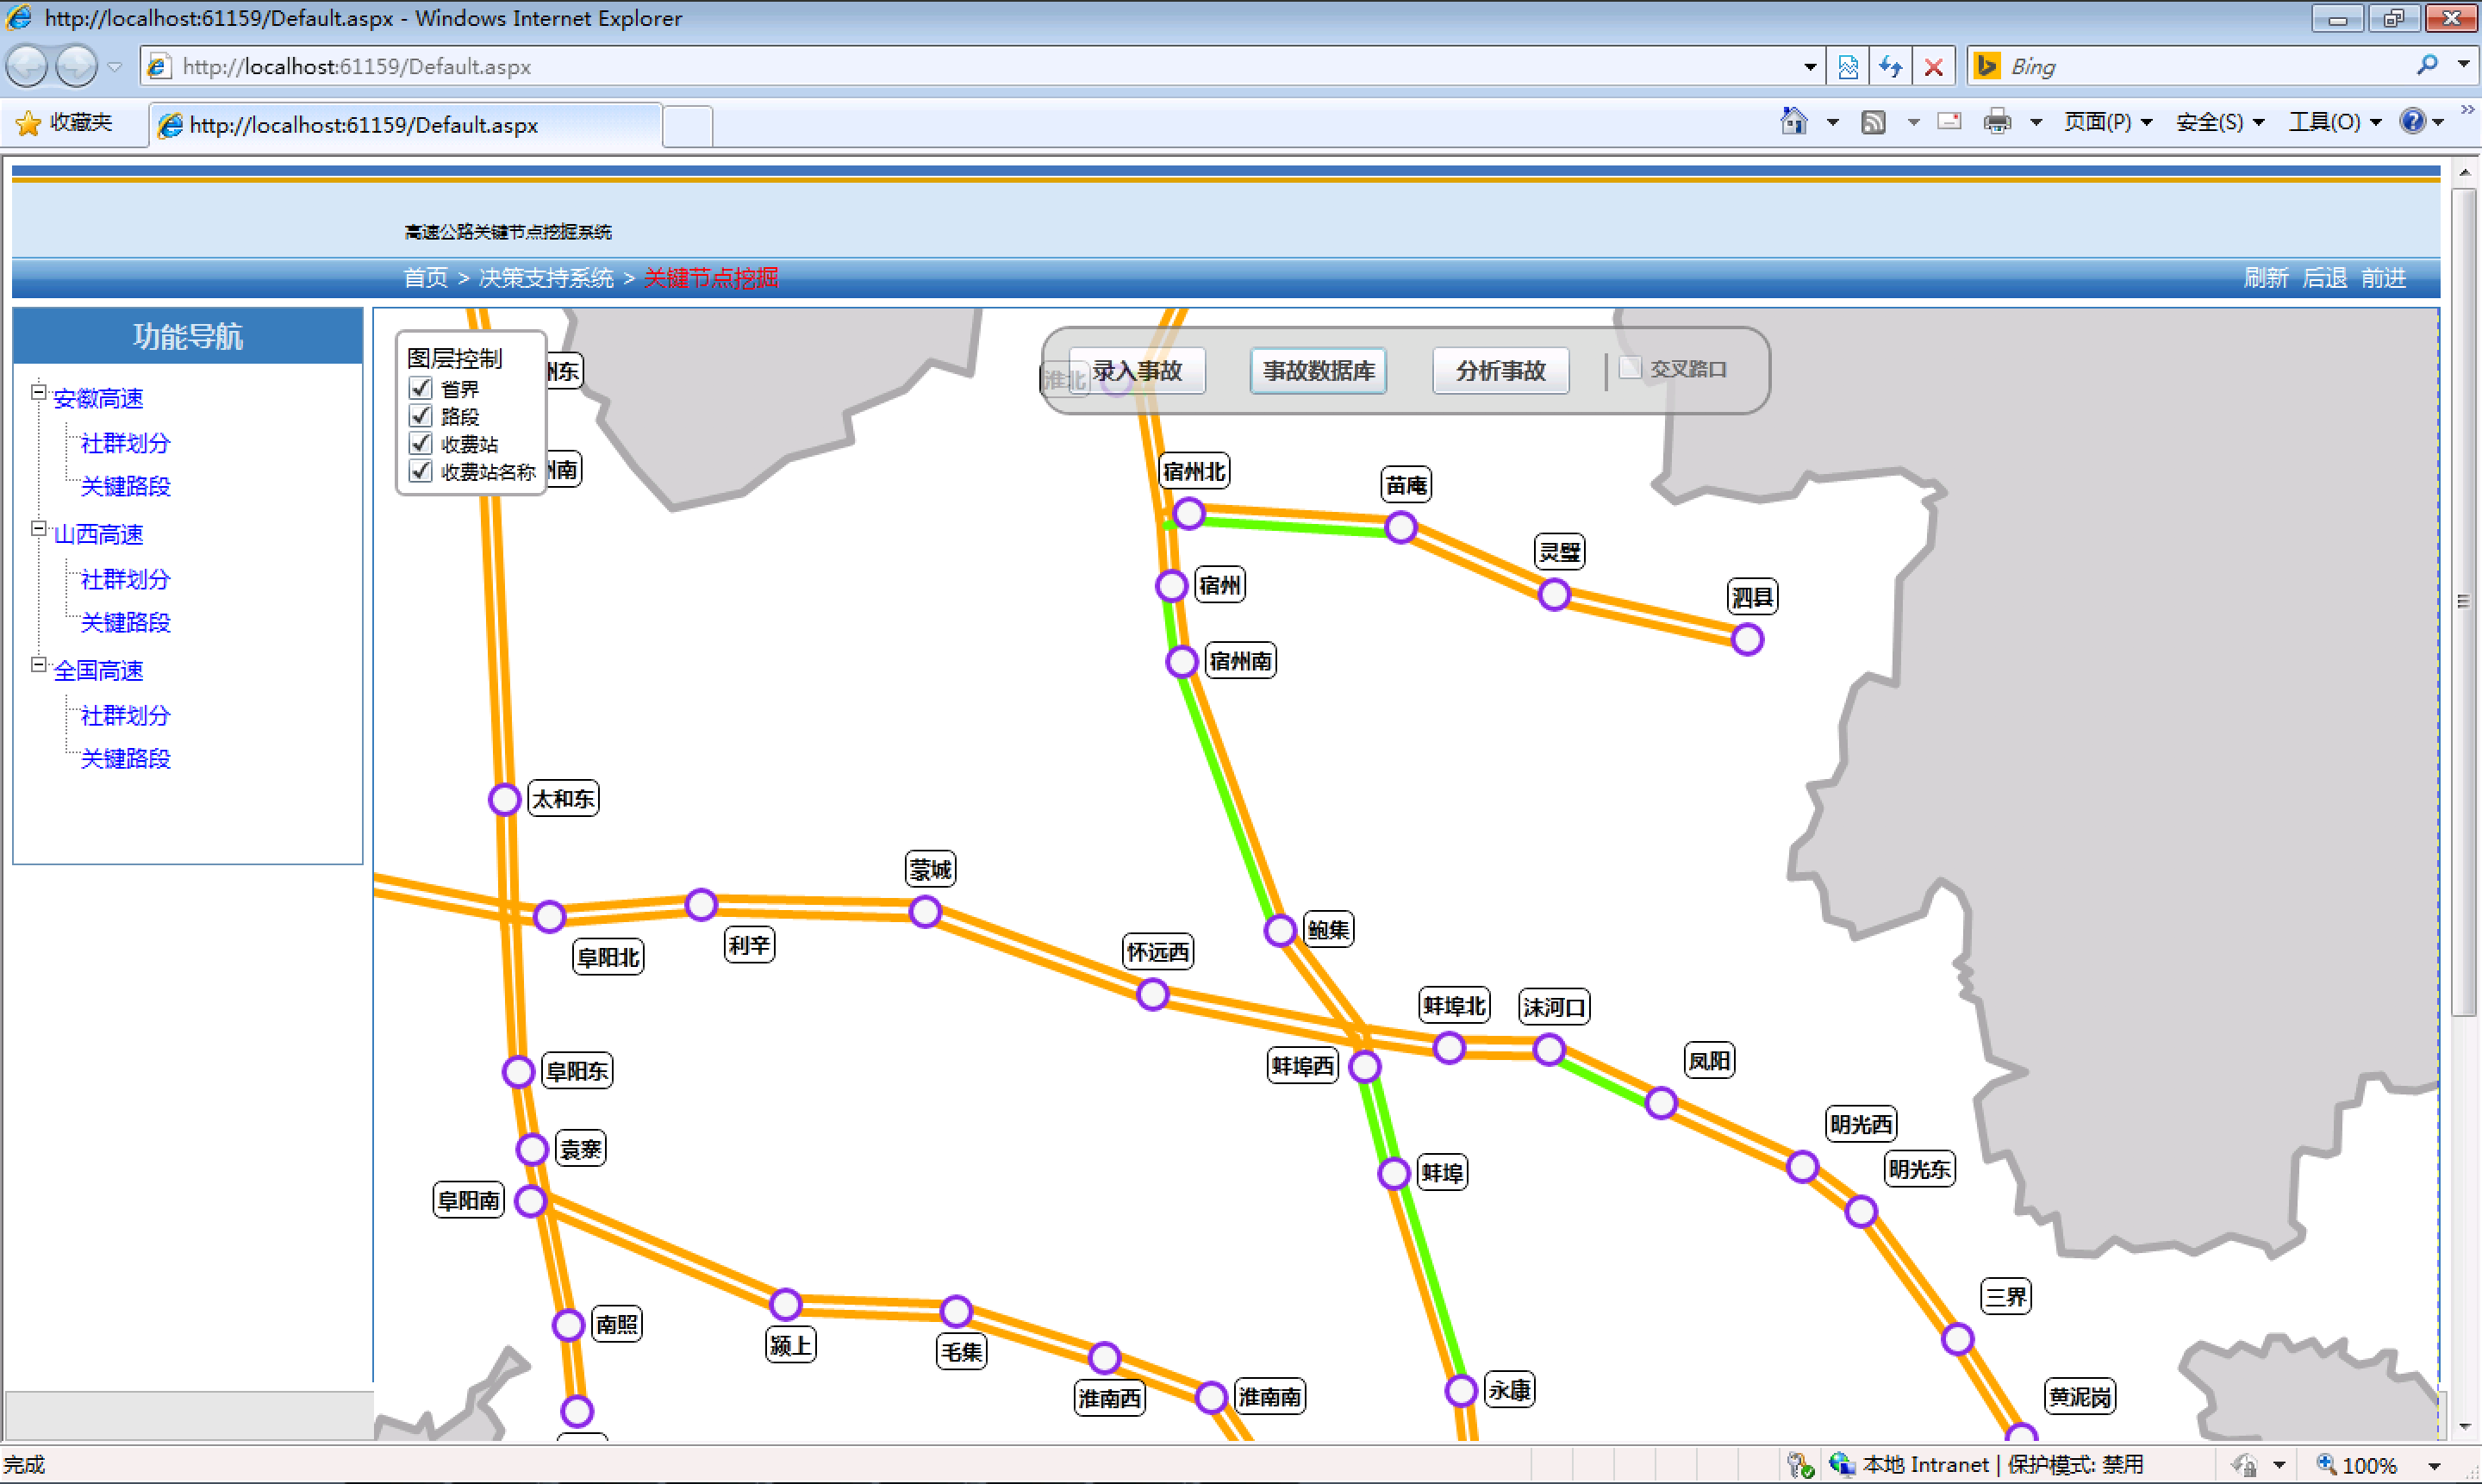
\includegraphics[width=4.4in]{picture/yuanxing2}
					\caption{系统路段选取结果图}
					\label{fig21}
				\end{minipage}%\
		\end{figure}

		目前系统只适用于安徽高速系统,但是系统可以扩展到任何具有收费站数据的中国高速公路上。

	\section{本章小结}
		本章介绍了一个面向高速公路的关键节点挖掘原型系统,给出了系统的流程图和样例图。该系统现在已经在安徽省高速公路网络上完全实现。该系统可扩展性强,所以可以很快的复用到其他省份乃至全国高速公路网络中。

	
	% 结论。
	% vim:ts=4:sw=4
% Copyright (c) 2014 Casper Ti. Vector
% Public domain.

\specialchap{总结与展望}
% 中文测试文字。
	交通系统中的关键节点识别非常重要。在高速公路系统中,关键节点的损毁会对整个系统的性能造成显著的影响,带来重大的经济损失。所以识别关键节点,在发生事故或者自然灾害之前进行维护巩固,在发生事故后进行快速修复,维护网络完整性非常重要。

	\subsection{主要工作}
		本文的主要工作和创新点如下:

		1)针对高速公路的实际特性,用概率来模拟高速公路的损毁情况,提出一种判定高速公路路段重要程度的研究模型。

			重要节点一般数量非常少, 但其影响却可以快速地波及到网络中大部分节点. 例如, 在对一个无标度网络的蓄意攻击中, 少量最重要节点被攻击就会导致整个网络瓦解;网络的“小世界特性”和“无标度特性”的发现掀起了网络科学持续 10 多年至今丝毫没有降温的研究热潮. 网络科学研究的热点逐渐从早期发现跨越 不同网络的宏观上的普适规律转变为着眼于从中观 (社团结构、群组结构)和微观层面(节点、链路)去解释不同网络所具有的不同特征。重要节点的挖掘研究也逐渐转为以微观研究为主。然而,从管理者的角度来说,过于微观的研究又无法体现高速公路系统的宏观特性。所以在此本文提出一种结合宏观(目标函数基于宏观理念)微观(基于路段损毁的随机规划问题)的高速公路关键路段挖掘模型,有效的解决了微观研究无法很好的顾及整体的问题。

		2)针对高速公路的空间物理特性,提出一种结合物理网络特性的复杂网络社群划分方法。

			传统的复杂网络社群划分与高速公路不同,首先高速公路是一种相当稀疏的复杂网络,网络中的拓扑结构特性不是很复杂;其次高速公路和普通的复杂网络不同,他的不同的节点之间具有物理空间距离,和其他复杂网络如社交网络中的距离概念不同。所以传统的复杂网络社群划分方法已经不再适用。在此引入可变权值方法,有效的解决了传统分群算法中的低分辨率特性以及极端退化特性。同时采用模拟退火思想加速模型收敛过程。
	\subsection{未来工作展望}

		本文工作虽然具有一定的创新性和实用性,但仍然存在一些局限和不足,需要在今后的研究中进一步探讨和完善,主要包括以下几个方面:

		1)由于时间限制,目前只在安徽路网上做完了原型系统。实际上安徽一个省的路网并不大,文中的优化方法也都是针对大规模路网提出的。所以下一步的工作就是将整个系统复用到全国的高速公路网络中去。

		2)目前分群算法尽量结合高速公路的物理空间特性,在分群效果上有一定的损失。现有的研究数据都是基于2010到2012年的历史数据进行研究,随着中国交通建设的不断完善,人们生活水平的不断提高,相信在高速公路上选择短途旅行的游客会越来越多。希望之后可以在最新的数据上进行研究,完善高速公路社群挖掘方法。



	% 正文中的附录部分。
	\appendix
	% 排版参考文献列表。
	\printbibliography[
		% 使“参考文献”出现在目录中;如果同时要使参考文献列表参与章节编号,
		% 可将“bibintoc”改为“bibnumbered”。
		heading = bibintoc,
		% 单独设定排序方案。此设定会局部覆盖之前的全局设置。
		% 注:只有同时使用 2.x 或之后版本的 biblatex 和相应兼容版本的 biber,
		% 才能对每个 \printbibliography 命令采用不同的排序方案,
		% 否则只能在载入 biblatex 宏包时就(全局)指定排序方案。
		% 在这样的情况下,请去掉所有的 sorting 选项,否则可能出错。
		% 此外,biblatex 3.0 中 \printbibliography 的 sorting 选项失效,
		% 详见 biblatex-caspervector 的文档。
		sorting = ecnty
	]
	% 各附录。
	% vim:ts=4:sw=4
% Copyright (c) 2014 Casper Ti. Vector
% Public domain.

\chapter{附件}
% 中文测试文字。
\pkuthssffaq



	% 以下为正文之后的部分,默认不进行章节编号。
	\backmatter
	% 致谢。
	% vim:ts=4:sw=4
% Copyright (c) 2014 Casper Ti. Vector
% Public domain.

\chapter{致谢}
% 中文测试文字。
时光荏苒,我的硕士生涯已接进尾声。这几年的时光既漫长又短暂,其中充满了酸甜苦辣,更有收获和成长。几年来,感谢陪我一起度过美好时光的每位尊敬的老师和亲爱的同学,正是你们的帮助,我才能克服困难,正是你们的指导,我才能解决疑惑,直到学业的顺利完成。

本人的学位论文是在我的恩师宋国杰副教授的殷切关怀和耐心指导下进行并完成的,衷心感谢我的恩师对我的淳淳教诲和悉心关怀。从课题的选择、项目的实施,直至论文的最终完成,宋老师都始终给予我耐心的指导和支持,我取得的每一点成绩都凝聚着恩师的汗水和心血。宋老师开阔的视野、严谨的治学态度、精益求精的工作作风,深深地感染和激励着我,在此谨向宋老师致以衷心的感谢和崇高的敬意。

感谢实验室的师弟师妹们,让我在最困难的时候看到你们的笑脸,被你们开朗的情绪感染。感谢你们带给我的帮助和鼓励!感谢一起打篮球的小伙伴,感谢谢老师组织的篮球活动,让我重新拾回篮球这一爱好。

最后,我要向百忙之中参与审阅、评议本论文各位老师、向参与本人论文答辩的各位老师表示由衷的感谢!人生的每个阶段都值得好好珍惜,这段美好岁月,因为有你们的关心和帮助,我很幸福。我会更加勤奋学习、认真研究,我会努力做得更好,我想这也是我能给你们的最好的回报吧。把最美好的祝福献给你们,愿永远健康、快乐!
	% 原创性声明和使用授权说明。
	% vim:ts=4:sw=4
%
% Copyright (c) 2008-2009 solvethis
% Copyright (c) 2010-2014 Casper Ti. Vector
% All rights reserved.
%
% Redistribution and use in source and binary forms, with or without
% modification, are permitted provided that the following conditions are
% met:
%
% * Redistributions of source code must retain the above copyright notice,
%   this list of conditions and the following disclaimer.
% * Redistributions in binary form must reproduce the above copyright
%   notice, this list of conditions and the following disclaimer in the
%   documentation and/or other materials provided with the distribution.
% * Neither the name of Peking University nor the names of its contributors
%   may be used to endorse or promote products derived from this software
%   without specific prior written permission.
%
% THIS SOFTWARE IS PROVIDED BY THE COPYRIGHT HOLDERS AND CONTRIBUTORS "AS
% IS" AND ANY EXPRESS OR IMPLIED WARRANTIES, INCLUDING, BUT NOT LIMITED TO,
% THE IMPLIED WARRANTIES OF MERCHANTABILITY AND FITNESS FOR A PARTICULAR
% PURPOSE ARE DISCLAIMED. IN NO EVENT SHALL THE COPYRIGHT HOLDER OR
% CONTRIBUTORS BE LIABLE FOR ANY DIRECT, INDIRECT, INCIDENTAL, SPECIAL,
% EXEMPLARY, OR CONSEQUENTIAL DAMAGES (INCLUDING, BUT NOT LIMITED TO,
% PROCUREMENT OF SUBSTITUTE GOODS OR SERVICES; LOSS OF USE, DATA, OR
% PROFITS; OR BUSINESS INTERRUPTION) HOWEVER CAUSED AND ON ANY THEORY OF
% LIABILITY, WHETHER IN CONTRACT, STRICT LIABILITY, OR TORT (INCLUDING
% NEGLIGENCE OR OTHERWISE) ARISING IN ANY WAY OUT OF THE USE OF THIS
% SOFTWARE, EVEN IF ADVISED OF THE POSSIBILITY OF SUCH DAMAGE.

% 原创性声明和使用授权说明页不需要装订到论文中,故不显示页码。
\cleardoublepage\thispagestyle{empty}
\newgeometry{height = 240mm, width = 150mm, ignoreheadfoot, vcentering}
{
	\vspace*{\fill}\linespread{1.5}\selectfont
	\centerline{\bfseries\Large 北京大学学位论文原创性声明和使用授权说明}

	\vskip 4em
	\centerline{\bfseries\Large 原创性声明}
	\vskip 1em

	本人郑重声明:
	所呈交的学位论文,是本人在导师的指导下,独立进行研究工作所取得的成果。
	除文中已经注明引用的内容外,
	本论文不含任何其他个人或集体已经发表或撰写过的作品或成果。
	对本文的研究做出重要贡献的个人和集体,均已在文中以明确方式标明。
	本声明的法律结果由本人承担。
	\vskip 1em
	\rightline
	{%
		论文作者签名:\hspace{5em}%
		日期:\hspace{2em}年\hspace{2em}月\hspace{2em}日%
	}

	\vskip 4em
	\centerline{\bfseries\Large 学位论文使用授权说明}
	\centerline{\zihao{-4}(必须装订在提交学校图书馆的印刷本)}
	\vskip 1em

	本人完全了解北京大学关于收集、保存、使用学位论文的规定,即:
	\begin{itemize}
		\item 按照学校要求提交学位论文的印刷本和电子版本;
		\item 学校有权保存学位论文的印刷本和电子版,
			并提供目录检索与阅览服务,在校园网上提供服务;
		\item 学校可以采用影印、缩印、数字化或其它复制手段保存论文;
		\item 因某种特殊原因需要延迟发布学位论文电子版,
			授权学校在 $\square$\nobreakspace{}一年 / %
			$\square$\nobreakspace{}两年 / %
			$\square$\nobreakspace{}三年以后在校园网上全文发布。
	\end{itemize}
	\par(保密论文在解密后遵守此规定)
	\vskip 1em
	\rightline
	{%
		论文作者签名:\hspace{5em}导师签名:\hspace{5em}%
		日期:\hspace{2em}年\hspace{2em}月\hspace{2em}日%
	}

	% 若需排版二维码,请将二维码图片重命名为“barcode”,
	% 转为合适的图片格式,并放在当前目录下,然后去掉下面 2 行的注释。
	%\vskip 4em \noindent
	%\includegraphics[height = 5em]{barcode}

	\vspace*{\fill}\par
}
\restoregeometry


\end{document}

